% !TeX spellcheck = de_DE
% !LuaLaTeX
\documentclass[12pt,a4paper,listof=totocnumbered,parskip=half,numbers=noenddot]{scrartcl}
\usepackage{scrhack}
\usepackage[ngerman]{babel}
\usepackage[T1]{fontenc}
\usepackage[utf8]{inputenc}
\usepackage{lmodern}
\usepackage{microtype}
\usepackage{geometry}
\geometry{a4paper, top=27mm, left=20mm, right=20mm, bottom=35mm, headsep=10mm, footskip=12mm}
\usepackage{setspace}
\usepackage{amsmath,amssymb,amsthm,mathrsfs,amsfonts}

\usepackage{csquotes}
\usepackage{booktabs}

\usepackage{graphicx}
\graphicspath{ {./img/} }
\usepackage{wrapfig}
% \usepackage{layouts}
\usepackage{textcomp} 
\usepackage[pdftex,dvipsnames]{xcolor}  % Coloured text etc.
\usepackage{svg}
\svgsetup{inkscapelatex=false, inkscapearea=drawing}
\usepackage[layout={margin,index},draft]{fixme}
\usepackage{rotating}
\usepackage{siunitx}

\usepackage[backend=biber,minbibnames=2,maxbibnames=2,maxcitenames=1,mincitenames=1,style=alphabetic]{biblatex}
\setcounter{biburlnumpenalty}{9000}
\setcounter{biburlucpenalty}{9000}
\setcounter{biburllcpenalty}{9000}

% new stretchable space between characters
\setlength{\biburlnumskip}{0mu plus 1mu}
\setlength{\biburlucskip}{0mu plus 1mu}
\setlength{\biburllcskip}{0mu plus 1mu}
\renewcommand{\namelabeldelim}{\addnbspace}

\addbibresource{Recherche/My Collection.bib}
\defbibheading{Literatur}{\section{Literaturverzeichnis}} 
\defbibheading{Quellen}{\subsection*{Quellenverzeichnis}} 

\DeclareSourcemap{
  \maps{
    \map{
      \step[fieldsource=url,
            match=\regexp{\$\\sim\$},
            replace=\regexp{\~}]
    }
  }
}

\usepackage{tikz}
\usetikzlibrary{calc,positioning, shapes, petri, automata,spy}
\usetikzlibrary{external}
\usepackage{pdfpages}
\usepackage{subcaption}
\usepackage{standalone}
\usepackage{multirow,tabularx}
\usepackage{xifthen}
\usepackage[hidelinks]{hyperref}
\usepackage[acronym,shortcuts,toc]{glossaries-extra}
%\usepackage{glossary-longbooktabs}
\setabbreviationstyle[acronym]{long-short} 

\renewcommand{\glsxtrregularfont}[1]{\textcolor{violet}{\glsxtrifwasfirstuse{\emph{#1}}{#1}}}
\renewcommand{\glsxtrabbreviationfont}[1]{\textcolor{teal}{\glsxtrifwasfirstuse{\emph{#1}}{#1}}}
% or
%\renewcommand{\glsxtrregularfont}[1]{\textcolor{violet}{\ifglsused{\glslabel}{#1}{\emph{#1}}}}
%\renewcommand{\glsxtrabbreviationfont}[1]{\textcolor{teal}{\ifglsused{\glslabel}{#1}{\emph{#1}}}}

\renewcommand*{\glsxtrsetupfulldefs}{%
  \renewcommand*{\glsxtrifwasfirstuse}[2]{##2}%
}

\usepackage{mathtools}


\usepackage{pgfplots}
\pgfplotsset{
	grid=major,
	width=\textwidth,
	height=5cm,
	compat=1.18,
	no markers,
  table/search path={performance/measurements},
}
\usepgfplotslibrary{external}
\tikzexternalize[prefix=tikz/,optimize command away=\includepdf]
%\tikzset{external/force remake}

\newcommand{\unsim}{\mathord{\sim}}
\newcommand{\e}{\ensuremath{\mathrm{e}}}

\newcommand{\R}{\ensuremath{\mathbb{R}}}
\newcommand{\N}{\ensuremath{\mathbb{N}}}
\newcommand{\F}{\ensuremath{\mathbb{F}}}
\newcommand{\Pot}{\ensuremath{\mathcal{P}}}

\DeclareMathOperator{\reachOp}{E}
\newcommand{\E}[1]{\reachOp(#1)}


\newcommand{\rowvec}[2]{\begin{pmatrix}
#1&#2\\
\end{pmatrix}}

\newcommand{\colvec}[2]{\begin{pmatrix}
#1\\
#2
\end{pmatrix}}

\newcommand{\deactivateGlossaries}
{
    \renewcommand{\makenoidxglossaries}{}
    \renewcommand{\printnoidxglossaries}{}
}

%\deactivateGlossaries

\makenoidxglossaries

\usepackage{listings}
\lstset{basicstyle=\footnotesize, captionpos=b, breaklines=true, showstringspaces=false, tabsize=2, frame=lines, numbers=left, numberstyle=\tiny, xleftmargin=2em, framexleftmargin=2em}
% \makeatletter
% \def\l@lstlisting#1#2{\@dottedtocline{1}{0em}{1em}{\hspace{1,5em} Lst. #1}{#2}}
% \makeatother

\definecolor{javared}{rgb}{0.6,0,0} % for strings
\definecolor{javagreen}{rgb}{0.25,0.5,0.35} % comments
\definecolor{javapurple}{rgb}{0.5,0,0.35} % keywords
\definecolor{javadocblue}{rgb}{0.25,0.35,0.75} % javadoc
\definecolor{gray}{rgb}{0.6,0.6,0.6}
 
\lstset{
	language=Java,
	basicstyle=\ttfamily\footnotesize,
	keywordstyle=\color{javapurple}\bfseries,
	stringstyle=\color{javared},
	commentstyle=\color{javagreen}\itshape\bfseries,
	morecomment=[s][\color{javadocblue}]{/**}{*/},
	numbers=left,
	numberstyle=\tiny\color{gray},
	stepnumber=1,
	numbersep=10pt,
	tabsize=3,
	showspaces=false,
	showstringspaces=false
}

\lstdefinestyle{inline}{
	basicstyle=\ttfamily\normalsize,
	keywordstyle=\ttfamily\normalsize,
	breaklines=true,
	breakatwhitespace=true%,
	%literate={A}{}{0\discretionary{}{A}{A}}
  %         {B}{}{0\discretionary{}{B}{B}}
  %         {C}{}{0\discretionary{}{C}{C}}
  %         {D}{}{0\discretionary{}{D}{D}}
  %         {E}{}{0\discretionary{}{E}{E}}
  %         {F}{}{0\discretionary{}{F}{F}}
  %         {G}{}{0\discretionary{}{G}{G}}
  %         {H}{}{0\discretionary{}{H}{H}}
  %         {I}{}{0\discretionary{}{I}{I}}
  %         {J}{}{0\discretionary{}{J}{J}}
  %         {K}{}{0\discretionary{}{K}{K}}
  %         {L}{}{0\discretionary{}{L}{L}}
  %         {M}{}{0\discretionary{}{M}{M}}
  %         {N}{}{0\discretionary{}{N}{N}}
  %         {O}{}{0\discretionary{}{O}{O}}
  %         {P}{}{0\discretionary{}{P}{P}}
  %         {Q}{}{0\discretionary{}{Q}{Q}}
  %         {R}{}{0\discretionary{}{R}{R}}
  %         {S}{}{0\discretionary{}{S}{S}}
  %         {T}{}{0\discretionary{}{T}{T}}
  %         {U}{}{0\discretionary{}{U}{U}}
  %         {V}{}{0\discretionary{}{V}{V}}
  %         {W}{}{0\discretionary{}{W}{W}}
  %         {X}{}{0\discretionary{}{X}{X}}
  %         {Y}{}{0\discretionary{}{Y}{Y}}
  %         {Z}{}{0\discretionary{}{Z}{Z}}
}

\newcommand{\code}[1]{\lstinline[style=inline]!#1!}
%TODO fix overfull hboxes LATER
\newcommand{\class}[1]{\code{#1}}
\newcommand{\const}[1]{\code{#1}}
\newcommand{\var}[1]{\code{#1}}

\lstset{escapeinside={(*}{*)}}

\newcommand{\LSset}[2]{\scriptsize $\begin{aligned}&\{#1\}_L\\&\{#2\}_S\end{aligned}$}


\tikzset{
    transV/.style={transition, fill=black, minimum height = 12mm, minimum width = 1.5mm,inner sep = 0mm},
    transH/.style={transition, fill=black, minimum width = 12mm, minimum height = 1.5mm,inner sep = 0mm},
    node distance=1.5
}

\DeclareSIUnit{\bit}{bit}
\DeclareSIUnit{\byte}{B}


\newcommand{\todo}[1]{\fxnote{{\color{red}#1}}}
\newcommand{\TODO}[2]{\fxnote*{{\color{red}#1}}{\underline{\emph{#2}}}}

\newlength{\wrapfigwidth}

\usepackage[headsepline,footsepline]{scrlayer-scrpage}
\renewcommand{\sectionmark}[1]{\markboth{\Ifnumbered{section}{Kapitel \thesection}{}}{#1}}
\renewcommand{\subsectionmark}[1]{}
\renewcommand{\subsubsectionmark}[1]{}
\lohead{\leftmark}
\rohead{\rightmark}
\chead[]{}
\lofoot{Entwicklung einer nebenläufigen Architektur für eine 3D-Spielebibliothek}
\cfoot[]{}
\rofoot{Seite \pagemark}
\pagestyle{scrheadings}
\setkomafont{pageheadfoot}{\small}
\newcommand{\memplot}[1]{ 
\begin{tikzpicture}
	\begin{axis}[
		xmin=0,
		xmax=65,
		ymin=0,
		ymax=2000,
    no markers,
    every axis plot post/.append style={
          % add the fill color to each `\addplot`
          % (`.` is an abbreviation for the "current color")
          fill=.!25,
					draw=none,
    },
		% we don't want to draw the axis lines etc. twice
		axis line style={draw=none},
		ticks=none,
		grid=major,
		grid style={help lines},
	]
			\addplot+[yellow] table[col sep=comma,header=true,x index=0, y index=4] {#1} \closedcycle;
			\addplot+[blue,stack plots=y] table[col sep=comma,header=true,x index=0, y index=1] {#1} \closedcycle;
			\addplot+[red,stack plots=y] table[col sep=comma,header=true,x index=0, y index=2] {#1}  \closedcycle;
	\end{axis}
	\begin{axis}[
		xmin=0,
		xmax=65,
		ymin=0,
		ymax=2000,
    no markers,
		grid=none,
		xlabel={Zeit (\si{\second})},
		ylabel={\ac{ram} (\si{\mega\byte})},
		legend entries = {Gesamt,Tenured,Eden},
		legend style={at={(0,1)},anchor=north west,xshift=.1cm,yshift=-.1cm,nodes={scale=.9}},
		]
			\addplot+[yellow] table[col sep=comma,header=true,x index=0, y index=4] {#1};
			\addplot+[blue,stack plots=y] table[col sep=comma,header=true,x index=0, y index=1] {#1};
			\addplot+[red,stack plots=y] table[col sep=comma,header=true,x index=0, y index=2] {#1};
	\end{axis}
\end{tikzpicture}
}

\newcommand{\fpsplot}[2][]{
	%\tikzset{external/remake next}
	\begin{tikzpicture}
			\begin{axis}[
			xlabel={Zeit (\si{\second})},
			xmin=0,
			ymin=0,
			xmax=65,
			ymax=600,
			ylabel={\si{\fps}},
			legend entries = {SystemA,SystemB},
			legend style={at={(0,1)},anchor=north west,xshift=.1cm,yshift=-.1cm,nodes={scale=.9}},
			#1
		]
				\addplot table[col sep=comma,header=true,x index=0, y index=2] {#2-single-fps.csv};
				\addplot table[col sep=comma,header=true,x index=0, y index=2] {#2-multi-fps.csv};
		\end{axis}
	\end{tikzpicture}
}

\newcommand{\cpuplot}[2][]{
	%\tikzset{external/remake next}
	\begin{tikzpicture}
			\begin{axis}[
			xlabel={Zeit (\si{\second})},
			xmin=0,
			xmax=65,
			ymin=0,
			ymax=100,
			ylabel={\ac{cpu} (\si{\percent})},
			legend entries = {SystemA,SystemB},
			legend style={at={(0,1)},anchor=north west,xshift=.1cm,yshift=-.1cm,nodes={scale=.9}},
			#1
		]
				\addplot table[col sep=comma,header=true,x index=0, y index=4] {#2-single-cpu.csv};
				\addplot table[col sep=comma,header=true,x index=0, y index=4] {#2-multi-cpu.csv};
		\end{axis}
	\end{tikzpicture}
}

\newcommand{\gpuplot}[2][]{
	%\tikzset{external/remake next}
	\begin{tikzpicture}
			\begin{axis}[
			xlabel={Zeit (\si{\second})},
			xmin=0,
			xmax=65,
			ymin=0,
			ymax=100,
			ylabel={\ac{gpu} (\si{\percent})},
			legend entries = {SystemA,SystemB},
			legend style={at={(0,1)},anchor=north west,xshift=.1cm,yshift=-.1cm,nodes={scale=.9}},
			#1
		]
				\addplot table[col sep=comma,header=true,x index=0, y index=7] {#2-single-gpu.csv};
				\addplot table[col sep=comma,header=true,x index=0, y index=7] {#2-multi-gpu.csv};
		\end{axis}
	\end{tikzpicture}
}
\newglossaryentry{na}{
first={\emph{nicht-atomar}},
name={nicht-atomar},
plural={nicht-atomare},
user1={nicht-atomaren},
description={Beschreibung einer Anweisung, die selbst aus weiteren Anweisungen besteht}
}

\newacronym[]{fps}{FPS}{Frames per second (dt. Bilder pro Sekunde)}
\DeclareSIUnit{\fps}{\ac{fps}}
\newacronym[]{sot}{SoT}{System on a Thread}
\begin{document}
\thispagestyle{empty}

\includegraphics[scale=0.2]{IM_Logo.pdf}
\begin{center}
	\vspace*{1cm}
	\Large
	\textbf{Konzeption, Integration und Performanceanalyse einer nebenläufigen Architektur für eine 3D-Spielebibliothek}\\
	\vspace*{2cm}
	\large
	An der Fakultät für Informatik und Mathematik der\\
	Ostbayerischen Technischen Hochschule Regensburg\\
	im Studiengang\\
	Informatik\\[2em]
	eingereichte\\
	\vspace*{1cm}
	\Large
	\textbf{Masterarbeit}\\[2em]
	\large
	zur Erlangung des akademischen Grades des\\
	Master of Science (M.Sc.)
	\vspace*{1cm}
	\Large

	\vfill
	\normalsize
	\begin{tabular}{rl}
	    \rule{0mm}{1ex}\textbf{Vorgelegt von:} & Florian Loher \\
		\rule{0mm}{1ex}\textbf{Matrikelnummer:} & \hspace*{-0.5em}\begin{tabular}[t]{r}3252714\end{tabular} \\ 
		~\\
		\rule{0mm}{1ex}\textbf{Erstgutachter:} & Prof.\ Dr.\ Carsten Kern \\ 
		\rule{0mm}{1ex}\textbf{Zweitgutachter:} & Prof.\ Dr.\ Daniel Jobst \\[2em]
		\rule{0mm}{1ex}\textbf{Abgabedatum:} & 21.\ April 2022 \\ 
	\end{tabular} 
\end{center}
\clearpage
\null\thispagestyle{empty}\clearpage
\markright{Inhaltsverzeichnis}
\tableofcontents\clearpage

\RedeclareSectionCommand[afterindent=no,runin=no,beforeskip=4pt,afterskip=0pt]{section}
\RedeclareSectionCommand[afterindent=no,runin=no,beforeskip=4pt,afterskip=-2pt]{subsection}
\RedeclareSectionCommand[afterindent=no,runin=no,beforeskip=4pt,afterskip=-4pt]{subsubsection}
\RedeclareSectionCommand[afterindent=no,beforeskip=4pt]{paragraph}

\pagebreak
\section{Einleitung}

\setstretch{1.15}

\subsection{Blocklib}
\subsection{Nebenläufige Programmierung}
\subsection{Testen und Testframeworks}

\pagebreak
\section{Grundlagen}
\subsection{Petri-Netze}\label{sec:petri}
Es gibt einige Ansätze zur Modellierung verteilter oder nebenläufiger Programme. Darunter finden sich auch Petri-Netze~\cite{Murata1989}. Mit einem Petrinetz kann ein modelliertes Programm mathematisch formal definiert und analysiert werden. Der Begriff Petri-Netz beschreibt auch eine Familie von verwandten Modellen. Das hier im Folgenden beschriebene Petri-Netz Modell wird auch Platz-Transitions-Netz (PT-Netz) genannt. Formal lässt sich ein PT-Netz $N$ als 5-Tupel $ N=(P,T,F,W,m_0)$ beschreiben. Dabei sind 
\begin{align*}
	&P  \quad \text{eine endliche Menge von Plätzen,}\\
	&T  \quad \text{eine endliche Menge von Transitionen,}\\
	&F \subseteq (P\times T) \cup (T \times P) \quad \text{die Menge der Relationen zwischen Plätzen und Transitionen,}\\
	&W: F \mapsto \N  \quad \text{eine Gewichtungsfunktion der Relationen und}\\
	&m_0: P \mapsto \N_0   \quad \text{die anfängliche Markierung der Plätze~\cite{Murata1989}.}\\
\end{align*}
Der durch ein PT-Netz beschriebene Graph kann auch grafisch dargestellt werden. Die Plätze $p \in P$ werden dabei als Kreise dargestellt, die Transitionen $ t \in T$ durch schwarz gefüllte Rechtecke, die Relationen $ f \in F$ durch gerichtete Kanten zwischen den Kreisen und Rechtecken, wobei die Elemente der Gewichtungsfunktion $W$ an die jeweiligen Kanten gesetzt werden. Die Markierung wird durch schwarze Punkte in den Plätzen dargestellt. Abbildun~\ref{fig:petrinet} zeigt ein simples Beispiel eines PT-Netzes  formal beschrieben (Abbildung~\ref{fig:petrinet:formal}) und seine grafische Repräsentation (Abbildung~\ref{fig:petrinet:graph}).
\begin{figure}
	\centering
	\begin{subfigure}[b]{.48\textwidth}
		$\begin{aligned}
			N &= (P,T,F,W,m_0)\\
			P &= \{p_1, p_2\}\\
			T &= \{t_1, t_2\}\\
			F &= \{(p_1, t_1), (p_2, t_2), (t_1, p_2)\}\\
			W &= \{((p_1, t_1),1), ((p_2, t_2),2), ((t_1, p_2), 1)\}\\
			m_0 &= \{(p_1, 1), (p_2, 0)\}
		\end{aligned}$
		\subcaption{}\label{fig:petrinet:formal}
	\end{subfigure}
	\hfill
	\begin{subfigure}[b]{.48\textwidth}
		\begin{tikzpicture}
			\node[place, label=$p_1$, tokens=1] (p1) at (0,0) {};
			\node[transV,label=$t_1$, right = of p1] (t1){};
			\node[place, label=$p_2$, right = of t1] (p2) {};
			\node[transV,label=$t_2$, right = of p2] (t2){};

			\draw 
			(p1) edge[post] node[above] {1} (t1)
			(t1) edge[post] node[above] {2} node[below=1cm] {$N$} (p2)
			(p2) edge[post] node[above] {1} (t2);
		\end{tikzpicture}
		\subcaption{}\label{fig:petrinet:graph}
	\end{subfigure}
	\caption{}\label{fig:petrinet}
\end{figure}

\subsubsection{Transitionsregel} Um nun das Verhalten von Programmen beschreiben zu können, kann die Markierung eines Petrinetzes anhand der folgenden sogenannten Transitions-Regel geändert werden~\cite{Murata1989}.
\begin{enumerate}
	\item Eine Transition $t_i \in T$ heißt \emph{aktiviert}, wenn für alle $(p,t_i) \in F $ gilt $ W((p,t_i)) \leq M(p)$ wobei $M$ die aktuelle Markierung ist. Es müssen also in allen Plätzen mit eingehenden Kanten genügend Marken bezüglich der Gewichtungsfunktion existieren. Diese Plätze werden auch \emph{Vorbedinungen} für die Transition genannt. Wenn ein Platz genügend Marken für eine Transition enthält, nennt man die Vorbedinung (bezüglich dieser Transition) \emph{erfüllt}.
	\item Eine aktivierte Transition kann, muss aber nicht \emph{feuern}.
	\item Feuert eine aktivierte Transition $t_i$, geht eine Markierung $M$ in eine Markierung $M'$ über. Dies erfolgt nach den folgenden Regeln.
	\begin{enumerate}
		\item $P$ wird in die disjunkten Mengen $P_\emptyset, P_\rightarrow, P_\leftarrow, P_\leftrightarrow$ unterteilt, wobei 
		\item $P_\emptyset = \{p \in P | (p,t_i) \notin F \land (t_i,p) \notin F\}$ die unbeteiligten Plätze sind,
		\item $P_\rightarrow = \{p \in P | (p,t_i) \in F \land (t_i,p) \notin F\}$ die Plätze mit eingehenden Kanten zur Transition,
		\item $P_\leftarrow = \{p \in P | (p,t_i) \notin F \land (t_i,p) \in F\}$ die Plätze mit ausgehenden Kanten aus der Transition und 
		\item $P_\leftrightarrow = \{p \in P | (p,t_i) \in F \land (t_i,p) \in F\}$ die Plätze mit eingehenden und ausgehenden Kanten.
		\item Dann gilt $
			M'(p) = \left\{ 
				\begin{aligned}
					& M(p) && \; , \; p \in P_\emptyset\\
					& M(p)-W((p,t_i)) && \; , \; p \in P_\rightarrow\\
					&M(p)+W((t_i,p)) && \; , \; p \in P_\leftarrow\\
					& M(p)-W((p,t_i))+W((t_i,p)) && \; , \; p \in P_\leftrightarrow
				\end{aligned}
				\right\}
		$
	\end{enumerate}
\end{enumerate}
Betrachtet man Abbildung~\ref{fig:petrinet} erneut, lässt sich erkennen, dass Transition $t_1$ aktiviert ist und Transition $t_2$ nicht, da in $p_2$ keine Marken sind.

\subsubsection{Erreichbarkeitsgraph}
Mittels der Transitionsregel lassen sich in einem Petri-Netz $N$ ausgehend von der Anfangsmarkierung $m_0$ gegebenenfalls weitere Markierungen erzeugen. Durch die wiederholte Anwendung der Transitionsregel auf alle daraus entstehenden Markierungen lässt sich ein Graph erstellen, der alle von der Anfangsmarkierung aus erreichbaren Markierungen erhält, den \emph{Erreichbarkeitsgraph} $\E{N}$ des Petri-Netzes.
\begin{figure}
	\begin{tikzpicture}[node distance=5mm,auto,state/.append style={rounded rectangle}]
		\node[state, initial] (q1) {$\{(p_1,1),(p_2,0)\}$};
		\node[state] (q2) [right=of q1] {$\{(p_1,0),(p_2,2)\}$};
		\node[state] (q3) [right=of q2] {$\{(p_1,0),(p_2,1)\}$};
		\node[state] (q4) [right=of q3] {$\{(p_1,0),(p_2,0)\}$};
		\path[->] 
		(q1) edge node {$t_1$} (q2)
		(q2) edge node {$t_2$} node[below=6mm] {Graph mit vollständigen Knotenbezeichnungen}(q3)
		(q3) edge node {$t_2$} (q4);

		\node[state,initial] (q5) [below=1.2cm of q1]{$(1,0)$};
		\node[state] (q6) [below=1.2cm of q2] {$(0,2)$};
		\node[state] (q7) [below=1.2cm of q3] {$(0,1)$};
		\node[state] (q8) [below=1.2cm of q4] {$(0,0)$};
		\path[->] 
		(q5) edge node {$t_1$} (q6)
		(q6) edge node {$t_2$} node[below=6mm] {Graph mit gekürzten Knotenbezeichnungen}(q7)
		(q7) edge node {$t_2$} (q8);
		\end{tikzpicture}
		\caption{Erreichbarkeitsgraph des Petri-Netzes aus Abbildung~\ref{fig:petrinet}. Der Graph ist zweimal dargestellt. Oben enthalten die Knoten des Graphen die vollständige Auszeichnung der Markierung, unten wird die Kurzschreibweise für die Knotenbezwichnungen genutzt, in der die Position den Platz kodiert. Der \enquote{start} Pfeil kennzeichnet die anfängliche Markierung.}\label{fig:reachability}
\end{figure}
In Abbildung~\ref{fig:reachability} wird der Erreichbarkeitsgraph des in Abbildung~\ref{fig:petrinet} dargestellten Petri-Netzes gezeigt. Die Knoten des Graphen sind die Markierungen des Petri-Netzes, die durch die Transitionsregel erreicht werden können. Da die Plätze des Petri-Netzes nummeriert sind, kann die Markierung verkürzt geschrieben werden, indem der Index des Tupels der Knotenbezeichnung den Platz beschreibt und die Zahl die Anzahl der Marken des Platzes kennzeichnet. In der Abbildung ist oben der Graph mit den vollständigen Markierungsbezeichnungen dargestellt. Unten wird die verkürzte Schreibweise genutzt.

ist die Anzahl der Marken pro Platz in jeder Markierung des Erreichbarkeitsgraphen maximal $1$, kann die Schreibweise weiter verkürzt werden, indem nur die Plätze beziehungsweise die Indizes der Plätze, die eine Marke enthalten genannt werden. Abbildung~\ref{fig:1-bpetrinet} zeigt eine Abwandlung des Petri-Netzes aus Abbildung~\ref{fig:petrinet}, das der gerade beschriebenen Eigenschaft entspricht, und den zugehörigen Erreichbarkeitsgraphen in verkürzter Schreibweise.
\begin{figure}
	\centering
	\begin{subfigure}[b]{.48\textwidth}
		\begin{tikzpicture}
			\node[place, label=$p_1$, tokens=1] (p1) at (0,0) {};
			\node[transV,label=$t_1$, right = of p1] (t1){};
			\node[place, label=$p_2$, right = of t1] (p2) {};
			\node[transV,label=$t_2$, right = of p2] (t2){};

			\draw 
			(p1) edge[post] node[above] {1} (t1)
			(t1) edge[post] node[above] {1} (p2)
			(p2) edge[post] node[above] {1} (t2);
		\end{tikzpicture}
		\subcaption{}\label{fig:1-bpetrinet:graph}
	\end{subfigure}
	\hfill
	\begin{subfigure}[b]{.48\textwidth}
		\begin{tikzpicture}[node distance=5mm,auto,state/.append style={rounded rectangle}]
			\node[state, initial] (q1) {$1$};
			\node[state] (q2) [right=of q1] {$2$};
			\node[state] (q3) [right=of q2] {};
			\path[->] 
			(q1) edge node {$t_1$} (q2)
			(q2) edge node {$t_2$} (q3);
		\end{tikzpicture}
		\subcaption{}\label{fig:1-bpetrinet:reachability}
	\end{subfigure}
\caption{}\label{fig:1-bpetrinet}
\end{figure} 

\subsubsection{Weitere Definitionen}
Um die Arbeit mit Petri-Netzen zu vereinfachen, werden nun noch einige weitere Definitionen eingeführt.

\begin{enumerate}
	\item Die Menge der Knoten mit Kanten zu einem Knoten $k \in P\cup T$ heißt \emph{Vorbereich} des Knotens $k$ und ist definiert als $^\circ k = \{v | (v,k) \in F\}$.
	\item Die Menge der Knoten mit Kanten von einem Knoten $k \in P\cup T$ heißt \emph{Nachbereich} des Knotens $k$ und ist definiert als $k^\circ  = \{n | (k,n) \in F\}$.
	\item Die Menge der Knoten einer Markierung $m$ mit mindesten $n$ Marken $\{x | m(x)\geq n\}$ wird $M_{\geq n}$ genannt.
	\item Das Maximum einer Markierung $m$, $\deg(m) \coloneqq \max \{m(p)|p\in P\}$, wird ihr \emph{Grad} genannt.
	\item Ein Petri-Netz $N$ heißt \emph{$n$-beschränkt}, wenn $n$ das Maximum der Grade der Markierungen des Erreichbarkeitsgraphen $(V,K)=\E{N}$ ist, also $n = \max\{\deg(m)| m\in V \}$.
	\item Gilt für eine Kante $((a, b),w) \in W$, dass $w = 1$, so kann im dazugehörigen Graphen die Beschriftung entfallen. Kanten ohne Beschriftung haben also ein implizites Gewicht von $1$.
\end{enumerate}



\subsubsection{Erweiterte Petri-Netze}
Um das Konzept von Variablenzugriffen einfacher zu modellieren führen \textcite{Goel1990} ein erweitertes Petri-Netz Modell ein. Dabei wird das 5-Tupel des Petri-Netzes um die folgenden Komponenten erweitert:
\begin{enumerate}
	\item eine Menge von Variablen $V$,
	\item eine Funktion $L: T \mapsto \Pot(V)$, die \emph{lesenden Zugriff} auf die Variablen modelliert, und
	\item eine Funktion $S: T \mapsto \Pot(V)$, die \emph{schreibenden Zugriff} auf die Variablen modelliert.
\end{enumerate}
$\Pot(V)$ ist dabei die Potenzmenge von $V$, also die Menge aller Teilmengen von $V$.
Ein Beispiel für ein erweitertes Petri-Netz, das ansonsten identisch zu dem Petri-Netz in Abbildung~\ref{fig:petrinet} ist, ist in Abbildung~\ref{fig:augpetrinet} gegeben. Die Formale Definition zeigt die neuen Mengen 
\begin{figure}
\centering
	\begin{minipage}[c]{.49\textwidth}
		$\begin{aligned}
			N &= (P,T,F,W,m_0, V, L, S)\\
			P &= \{p_1, p_2\}\\
			T &= \{t_1, t_2\}\\
			F &= \{(p_1, t_1), (p_2, t_2), (t_1, p_2)\}\\
			W &= \{((p_1, t_1),1), ((p_2, t_2),2), ((t_1, p_2), 1)\}\\
			m_0 &= \{(p_1, 1), (p_2, 0)\}\\
			V &= \{a,b\}\\
			L &= \{(t_1,\{a,b\}), (t_2,\emptyset)\}\\
			S &= \{(t_1,\{a\}), (t_2,\emptyset)\}
		\end{aligned}$
	\end{minipage}
	\hfill
	\begin{minipage}[c]{.49\textwidth}
		\begin{tikzpicture}
			\node[place, label=$p_1$, tokens=1] (p1) at (0,0) {};
			\node[transV,label=$t_1$, right = of p1, label=below:{\LSset{a,b}{a}}] (t1){};
			\node[place, label=$p_2$, right = of t1] (p2) {};
			\node[transV,label=$t_2$, right = of p2] (t2){};

			\draw 
			(p1) edge[post] node[above] {1} (t1)
			(t1) edge[post] node[above] {2} node[below=2cm] {$N$} (p2)
			(p2) edge[post] node[above] {1} (t2);
		\end{tikzpicture}
	\end{minipage}
	\caption{Beispiel eines erweiterten Petri-Netzes. Links ist die formale Definition gegeben, rechts der dazugehörige Graph. In Platz $p_2$ wird auf die Variablen $a$ und $b$ lesend zugegriffen und auf Variable $a$ schreibend.}\label{fig:augpetrinet}
\end{figure}
Nachdem nun die formalen Grundlagen gelegt sind, werden in diesem Abschnitt Grundbegriffe eingeführt, die notwendig für das Verständnis der nächsten Kapitel sind. Besonders wichtig sind insbesondere die Begriffe \enquote{Thread}, \enquote{Nebenläufigkeit} und \enquote{Wettkampfbedingung}, da diese Begriffe in der Arbeit intensiv behandelt werden.


\subsubsection{Definition von Thread}
Um definieren zu können, was ein Thread ist, müssen zuerst einige weitere Grundbegriffe eingeführt werden. 

Als \gls{Programm} wird in dieser Arbeit die konkrete Niederschrift eines Algorithmus bezeichnet. Die Elemente, aus denen das \gls{Programm} besteht, werden als \glspl{Anweisung} bezeichnet. Bei der Ausführung eines \glsuseri{Programm} werden Einzelschritte durchlaufen, diese bezeichnet man als \glspl{Aktivitaet}. Eine Sequenz von \glspl{Aktivitaet}, die ein isoliertes Problem abarbeitet, wird \emph{Prozess} genannt. Um diese Definition des Prozessbegriffs von späteren Definitionen abzugrenzen wird er im Folgenden \gls{Rechenprozess} genannt. Die Ausführungseinheit, auf der die Schritte eines \glsuseri{Rechenprozess} durchgeführt werden, wird \emph{Prozessor} genannt~\cite[S.~22]{Herrtwich1989}. In der Regel besitzt ein Rechner, beispielsweise ein PC, mehrere Ausführungseinheiten. Bei PCs gibt es eine Recheneinheit, die üblicherweise die meisten \glspl{Rechenprozess} ausführt und andere Prozessoren koordiniert, den \ac{cpu}.

Wenn ein \gls{Programm} auf einem Betriebssystem ausgeführt wird, erzeugt das Betriebssystem einen isolierten Adressraum, in dem das \gls{Programm} ausgeführt wird. Ein \gls{Rechenprozess}, der auf diese Weise ausgeführt wird, wird in dieser Arbeit als \emph{(System-)Prozess} bezeichnet. \textcite[Kapitel~2]{Tanenbaum2016} liefern eine gute Übersicht über Systemprozesse, dort als Prozesse bezeichnet. Systemprozesse können selbst weitere Systemprozesse starten, wenn das Betriebssystem dies zulässt. Diese Systemprozesse besitzen dann ihren eigenen Adressraum. Die Anzahl der Systemprozesse, die auf einem Rechner laufen, ist meist höher als die Anzahl der Prozessoren des Rechners. Somit können nicht alle Prozesse zur gleichen Zeit ausgeführt werden. Damit dennoch alle Prozesse voranschreiten können, wechseln moderne Betriebssysteme die Systemprozesse, die auf den Prozessoren des Rechners ausgeführt werden, in schneller Folge. Dabei muss das Betriebssystem einige zu den Systemprozessen gehörende Daten, den \emph{Prozesskontrollblock}, tauschen, sodass der jeweils gerade ausführende Systemprozess seinen eigenen Prozesskontrollblock zur Verfügung hat. Dieser Tausch wird \emph{Kontextwechsel} genannt~\cite[S.~59]{Tanenbaum2016}.

Das Speichern und Laden der Prozesskontrollblöcken im Rahmen der Kontextwechsel von Systemprozessen benötigt eine nicht zu vernachlässigende Menge an Zeit. Dieser Zeitverbrauch wird auch als \emph{Overhead} bezeichnet. Um den Overhead von Kontextwechseln zu vermindern, bieten moderne Betriebssysteme Systemprozessen die Möglichkeit \glspl{Rechenprozess} zu erzeugen, die denselben Adressraum wie der erzeugende Systemprozess besitzen. Ein auf diese Art erzeugter \gls{Rechenprozess} heißt \emph{Thread}. Da die Menge der thread-eigenen Daten, des \emph{Threadkontrollblocks}, deutlich geringer ist als die des Prozesskontrollblocks, erzeugt der Kontextwechsel zwischen Threads einen geringeren Overhead. Zudem können Threads aufgrund des gemeinsamen Adressraums einfacher auf geteilte Ressourcen zugreifen. Das vereinfacht die Kooperation zwischen diesen \glsuserii{Rechenprozess}~\cite[S.~139~ff.]{Tanenbaum2016}.

\paragraph{Anweisungen und Petri-Netze}
Um formal Eigenschaften eines \glsuseri{Programm} zu beschreiben, ist es möglich dieses mittels eines Petri-Netzes (automatisiert) zu modellieren. Dazu müssen Petri-Netz-Konstrukte genutzt werden, die die \glspl{Anweisung} des \glsuseri{Programm} abbilden können. Für die Analyse nebenläufiger \glspl{Programm} sind nur sogenannte \emph{Rendezvous}-\glspl{Anweisung} sowie Kontrollstrukturen relevant~\cite{Goel1990}. Für diese lassen sich Unter-Petri-Netze definieren, die deren Verhalten modellieren. Eine Anweisung entspricht dann einem bestimmten Unter-Petri-Netze. Eine Auflistung für die Modellierung nebenläufiger \glspl{Programm} benötigter Unter-Petri-Netze ist in \cite{Goel1990} zu finden.  Da die Modellierung von Verzweigungen durch Unter-Petri-Netze in \cite[Abbildung 3.1]{Goel1990} semantisch nicht ganz korrekt ist, wird sie in Abbildung~\ref{fig:supnetifelse} korrigiert dargestellt. 
\begin{figure}
	\centering
	\begin{tikzpicture}[node distance=2cm,on grid, auto]
		\node[place, label=$p_1$] (p1) {};
		\node[transV, label=\texttt{if}, above right = of p1] (if) {};
		\node[transV, label=\texttt{else},below right = of p1] (else) {};
		\node[right = of if] (dots1){$\dots$};
		\node[right = of else] (dots2){$\dots$};
		\node[place, label=$p_2$, right = of dots1] (p2) {};
		\node[place, label=$p_3$, right = of dots2] (p3) {};
		\node[transV, label=$t_1$, right = of p2] (t1) {};
		\node[transV, label=$t_2$, right = of p3] (t2) {};
		\node[place, label=$p_4$, below right = of t1] (p4) {};
		\node[transV, label=\texttt{end if}, right = of p4] (endif) {};
	
	
	
		\draw 
		(p1) edge[post] (if)
		(p1) edge[post] (else)
		(if) edge[post] (dots1)
		(else) edge[post] (dots2)
		(dots1) edge[post] (p2) 
		(dots2) edge[post] (p3) 
		(p2) edge[post] (t1)
		(p3) edge[post] (t2)
		(t1) edge[post] (p4)
		(t2) edge[post] (p4)
		(p4) edge[post] (endif)
		;
	\end{tikzpicture}
	\caption[Semantisch korrigiertes Unter-Petri-Netz zu Modellierung von Verzweigungen.]{Semantisch korrigiertes Unter-Petri-Netz zu Modellierung von Verzweigungen nach \cite[Abbildung~3.1]{Goel1990}.}\label{fig:supnetifelse}
\end{figure}

Die Plätze $p_1,p_2,p_3,p_4$ und die Transitionen $t_1,t_2$ sind Hilfselemente die die semantische Korrektheit der Transitionen \code{if}, \code{else} und \code{end if} sicherstellen. Eine Markierung kann exklusiv nur von \code{if} oder von \code{else} zum Feuern verwendet werden. Durch die Transitionen $t_1$ und $t_2$ entsteht eine Markierung in $p_5$ wodurch \code{end if} feuern kann egal ob anfangs \code{if} oder \code{else} gefeuert hat. $p_2$ und $p_3$ existierten, damit das Petri-Netz ein bipartiter Graph bleibt, sich also immer Plätze und Transitionen \enquote{abwechseln}. Die Modellierung eines \code{switch}-Statements erfolgt analog, indem die Anzahl der Pfade zwischen $p_1$ und $p_4$ angepasst wird.

\subsubsection{Nebenläufigkeit}\label{sec:nebenl}
Im vorherigen Abschnitt wurde beschrieben, dass verschiedene \glspl{Rechenprozess} unabhängig von einander \enquote{gleichzeitig} ablaufen können. Dieses \enquote{gleichzeitig} wird jetzt genauer beleuchtet. Ein \gls{Programm} wird häufig als \emph{Sequenz} von \glspl{Anweisung} verstanden. In der Definition von \gls{Programm} in dieser Arbeit wird bewusst auf das Wort Sequenz verzichtet, denn bei vielen \glsuserii{Programm} kann es bei bestimmten \glspl{Anweisung} irrelevant sein, in welcher Reihenfolge oder ob sie sogar gleichzeitig ausgeführt werden. Man betrachte das folgende \gls{Programm} in Listing~\ref{lst:squareSeqEx}, das die Quadratsumme zweier Ganzzahlen (im Folgenden auch Quadratsumme genannt) ausgibt.

\begin{lstlisting}[caption={[Beispiel eines \glsentryuseri{Programm} das sequentiell die Summe von Quadraten zweier Ganzzahlen berechnet.]Beispiel eines \glsuseri{Programm} das die Summe von Quadraten zweier Ganzzahlen berechnet. Die Berechnung der Quadratzahlen wird nacheinander in einer fest definierten Sequenz durchgeführt.}, label={lst:squareSeqEx},float={!htbp}]
printSummedSquare(int a, int b){
  x <- a*a (*\label{lst:squareSeqEx:aa}*)
  y <- b*b (*\label{lst:squareSeqEx:bb}*)
  print(x+y) (*\label{lst:squareSeqEx:print}*)
}
\end{lstlisting}
Es ist leicht zu erkennen, dass es vollkommen egal ist, ob zuerst \code{x} oder \code{y} ausgerechnet wird oder die Berechnungen simultan stattfinden. Einzig der Ausgabebefehl in Zeile~\ref{lst:squareSeqEx:print} darf erst ausgeführt werden, nachdem \code{x} und \code{y} berechnet wurden. Zuzulassen, dass die Ausführreihenfolge in dem \gls{Programm} nicht definiert ist, führt dazu, dass das \gls{Programm} präziser der Problembeschreibung \enquote{gib die Quadratsumme zweier Ganzzahlen aus} entspricht, und ermöglicht auch eine potenziell schnellere Berechnung, da die Quadrate gleichzeitig berechnet werden können.

Paare oder Gruppen von \glspl{Anweisung}, die gleichzeitig oder in beliebiger Reihenfolge ausgeführt werden, heißen \emph{nebenläufig}. Da die Ausführungsreihenfolge der Anweisungen in Zeile~\ref{lst:squareSeqEx:aa} und Zeile~\ref{lst:squareSeqEx:bb} egal ist, dürfen diese Anweisungen auch nebenläufig definiert sein.

Eine der obigen Problemstellung, \enquote{gib die Quadratsumme zweier Ganzzahlen aus}, nähere Implementierung der Quadratsumme könnte unter Nutzung von Nebenläufigkeit wie Listing~\ref{lst:squareConcEx} aussehen. Dabei wird auf die Schreibweise von \textcite[S.~16]{Herrtwich1989} zurückgegriffen.
\begin{lstlisting}[caption={[Beispiel eines \glsuseri{Programm} mit nebenläufigem Code in einem \code{conc}-Block.]Beispiel eines \glsuseri{Programm} mit nebenläufigem Code in einem \code{conc}-Block. Das \gls{Programm} gibt die Summe von zwei Quadratzahlen aus, wobei die Berechnung der Quadratzahlen nebenläufig stattfindet.}, label={lst:squareConcEx},float={!htbp}]
printSummedSquare(int a, int b){
  conc 
    x <- a*a ||
    y <- b*b
  conc end
  print(x+y)
}
\end{lstlisting}
In einem \code{conc}-Block, definiert durch \code{conc} und \code{conc end}, sind alle \glspl{Anweisung}, die durch \code{||} getrennt sind, als nebenläufig zu verstehen. 

Wie man an dem Beispiel in Listing~\ref{lst:squareConcEx} erkennen kann, beschäftigt sich Nebenläufigkeit besonders mit der Struktur und der Möglichkeit der Zusammensetzung voneinander unabhängiger \glspl{Anweisung}. Somit ist es Aufgabe der nebenläufigen Programmierung, Probleme oder Aufgaben in unabhängige Teile zu zerlegen und zu strukturieren~\cite{Pike2012,Hettel2016}. Blöcke von \glspl{Anweisung}, die (bezüglich der Aufgabe) nebenläufig sein könnten, aber als Anweisungssequenz definiert sind (siehe Listing~\ref{lst:squareSeqEx} Zeile 2 und 3), werden in dieser Arbeit als \emph{pseudo-sequentialisiert} bezeichnet.

Bei der Definition nebenläufiger Anweisungen ist allerdings Vorsicht geboten, da sichergestellt werden muss, dass zwei Anweisungen auch tatsächlich nebenläufig sein dürfen. Eine \gls{Anweisung} kann beispielsweise durch einen Compiler in mehrere \glspl{Anweisung} geteilt werden oder selbst schon aus mehreren \glspl{Anweisung} bestehen (man denke zum Beispiel an Funktionsaufrufe). Solche \glspl{Anweisung} werden \gls{nichtAtomar} genannt. Eine Menge von nebenläufigen \glspl{Anweisung}, von denen mindestens eine \gls{nichtAtomar} ist, kann \emph{verzahnt} ausgeführt werden. Eine Ausführung von \glspl{Anweisung} ist verzahnt, wenn zwischen der Ausführung der Teile einer \glsuseri{nichtAtomar} \gls{Anweisung} andere \glspl{Anweisung} ausgeführt werden. Abbildung \ref{fig:concAnweisungen} zeigt zur Veranschaulichung die verschiedenen Möglichkeiten, wie zwei nebenläufige \glspl{nichtAtomar} \glspl{Anweisung} im Zeitverlauf ausgeführt werden können, sowohl auf einem Prozessor als auch auf zwei Prozessoren. Dadurch kann es passieren, dass Anweisungen, die zuerst den Anschein haben, nebenläufig sein zu können, nicht nebenläufig sein dürfen, weil eine verzahnte Ausführung der zugehörigen Aktivitäten ein unerwünschtes Ergebnis liefern würde. 

\begin{figure}[hbt]
	\centering
\newlength\aOne
\newlength\aTwo
\newlength\aThree
\newlength\bOne
\newlength\bTwo
\pgfmathsetlength{\aOne}{2cm}
\pgfmathsetlength{\aTwo}{2.25cm}
\pgfmathsetlength{\aThree}{2.5cm}
\pgfmathsetlength{\bOne}{2.75cm}
\pgfmathsetlength{\bTwo}{3cm}
\begin{subfigure}{\textwidth}
	\centering
\begin{tikzpicture}

	\draw[->] (0,0) -- (13,0) node[right] {Zeit};
	
	\node[draw,fill=red, anchor=south west, minimum width = \aOne] at (0, .5) (A1) {A Teil1};

	\node[draw,fill=red, anchor=west, minimum width = \aTwo] at (A1.east) (A2) {A Teil2};
	\node[draw,fill=red, anchor=west, minimum width = \aThree] at (A2.east) (A3) {A Teil3};
	
	\node[draw,fill=cyan, anchor=south west, minimum width = \bOne] at (0, 1.5) (B1) {B Teil1};
	\node[draw,fill=cyan, anchor=west, minimum width = \bTwo] at (B1.east) (B2) {B Teil2};

	\node[anchor=east] at (B1.west) {Prozessor 1};
	\node[anchor=east] at (A1.west) {Prozessor 2};
\end{tikzpicture}
\subcaption{Gleichzeitige Ausführung der \glspl{Anweisung} A und B auf zwei Prozessoren}
\end{subfigure}
\\[1.5em]
\begin{subfigure}{\textwidth}
	\centering
\begin{tikzpicture}

	\draw[->] (0,0) -- (13,0) node[right] {Zeit};
	
	\node[draw,fill=cyan, anchor=south west, minimum width = \bOne] at (0, .5) (B1) {B Teil1};
	\node[draw,fill=cyan, anchor=west, minimum width = \bTwo] at (B1.east) (B2) {B Teil2};
	\node[draw,fill=red, anchor=west, minimum width = \aOne] at (B2.east) (A1) {A Teil1};
	\node[draw,fill=red, anchor=west, minimum width = \aTwo] at (A1.east) (A2) {A Teil2};
	\node[draw,fill=red, anchor=west, minimum width = \aThree] at (A2.east) (A3) {A Teil3};

	\node[anchor=east] at (B1.west) {Prozessor 1};
\end{tikzpicture}
\subcaption{Sequenzielle Ausführung der \glspl{Anweisung} A und B auf einem Prozessor}
\end{subfigure}
\\[1.5em]
\begin{subfigure}{\textwidth}
	\centering
\begin{tikzpicture}

	\draw[->] (0,0) -- (13,0) node[right] {Zeit};
	
	\node[draw,fill=cyan, anchor=south west, minimum width = \bOne] at (0, .5) (B1) {B Teil1};
	\node[draw,fill=red, anchor=west, minimum width = \aOne] at (B1.east) (A1) {A Teil1};
	\node[draw,fill=red, anchor=west, minimum width = \aTwo] at (A1.east) (A2) {A Teil2};
	\node[draw,fill=cyan, anchor=west, minimum width = \bTwo] at (A2.east) (B2) {B Teil2};
	\node[draw,fill=red, anchor=west, minimum width = \aThree] at (B2.east) (A3) {A Teil3};

	\node[anchor=east] at (B1.west) {Prozessor 1};
\end{tikzpicture}
\subcaption{Verzahnte Ausführung der \glspl{Anweisung} A und B auf einem Prozessor}
\end{subfigure}

\caption[Mögliche Ausführungen nebenläufiger \glsentryplural{Anweisung}.]{Mögliche Ausführungen nebenläufiger \glspl{Anweisung}. Die Grafik bildet eine Abbildung aus \cite{Herrtwich1989} nach.}\label{fig:concAnweisungen}
\end{figure}

Werden nebenläufige \glspl{Anweisung} parallel ausgeführt, spricht man auch von \emph{Multiprocessing}. Handelt es sich bei den Prozessen um Threads, wird der Begriff \emph{Multithreading} genutzt.

\paragraph{Nebenläufigkeit und Petri-Netze}
Um ein eindeutiges Verständnis des hier genutzten Begriffs der Nebenläufigkeit zu geben, wird dieser auch in Bezug auf Petri-Netze definiert. Wichtig anzumerken ist, dass der hier beschriebene Begriff von dem üblichen Verständnis der Nebenläufigkeit in Petri-Netzen abweicht. 

Normalerweise werden Petri-Netze als inhärent nebenläufig verstanden, da durch die Transitionsregel zu jeder Zeit jede beliebige Transition feuern kann, deren Vorbedingungen erfüllt sind. Der hier verwendete Begriff bezieht sich allerdings darauf, dass \glspl{Anweisung} unabhängig voneinander, ohne sich gegenseitig zu beeinflussen, ausführbar sind. Das Feuern einer Transition kann aber den Vorbereich einer anderen Transition verändern, wodurch sie beeinflusst wird.

In dieser Arbeit heißen zwei Transitionen $t_1, t_2$ eines Petri-Netzes $N$ genau dann nebenläufig, wenn ${}^\circ t_1 \cap {}^\circ t_2 = \emptyset$ gilt und eine Markierung $m_\text{conc}$ im Erreichbarkeitsgraphen $\E{N}$ existiert, in der sowohl $t_1$ als auch $t_2$ aktiviert sind. Die Vorbereiche der Transitionen dürfen sich also nicht überschneiden.

\subsubsection{Folgen von Nebenläufigkeit}\label{sec:nebenl-folgen}
Wie in Abschnitt \ref{sec:nebenl} beschrieben, muss ein \gls{Programm} keine Sequenz von \glspl{Anweisung} sein, sondern kann auch nebenläufige \glspl{Anweisung} enthalten. Diese Möglichkeit hat eine Reihe von Folgen, die es bei der nebenläufigen Programmierung zu beachten gilt.
\paragraph{Nichtdeterminismus}
Enthält ein \gls{Programm} nebenläufige \glspl{Anweisung}, ist die Reihenfolge der daraus resultierenden \glspl{Aktivitaet} nicht definiert und kann sich bei jedem Programmdurchlauf ändern. Die Ausführung ist also \emph{nichtdeterministisch}, als direkte Folge der Nebenläufigkeit~\cite[S.~17~f.]{Herrtwich1989}. Erwartet man von einem \gls{Programm} \emph{Determiniertheit}\footnote{Es kann durchaus sein, dass Determiniertheit in einem \gls{Programm} nicht gewünscht ist. Man betrachte beispielsweise ein \gls{Programm}, das einen echten Zufallsgenerator beschreibt. Hier wäre Determiniertheit ein direkter Widerspruch zur Aufgabe des \glsuseri{Programm}.}, also die Eigenschaft, dass gleiche Eingaben immer zu den gleichen Ausgaben führen, ist Nichtdeterminismus in der Regel zu vermeiden. Determiniertheit kann aber auch bei einem Verzicht auf Determinismus sichergestellt werden. Liefert ein \gls{Programm} bei jeder beliebigen Ausführreihenfolge dasselbe Ergebnis, ist es trotz Nichtdeterminismus weiterhin determiniert, weil die Ausführreihenfolge für das Ergebnis keine Rolle spielt~\cite[S.~18~f.]{Herrtwich1989}. 
\paragraph{Nichtreproduzierbarkeit}
Da das Wissen und die Kontrolle über die Ausführreihenfolge abgegeben wird, wird die Nachvollziehbarkeit des Programmablaufs erschwert~\cite[S.~20]{Herrtwich1989}. Tritt beispielsweise ein Fehler auf, kann im Nachhinein nicht ermittelt werden, was die Ausführreihenfolge war, die zu dem Fehler geführt hat. Dasselbe Problem ergibt sich ebenfalls, wenn ein nichtdeterminiertes \gls{Programm} eine Lösung ausgibt und nachvollzogen werden soll, welche Ausführreihenfolge zu diesem Ergebnis geführt hat. Insbesondere das Testen und Debugging von Software wird dadurch erschwert, da es unmöglich ist bei jedem Test dieselben Bedingungen herzustellen, sodass beispielsweise Tests Fehler nicht verlässlich aufzeigen, weil diese nur bei bestimmten Ausführreihenfolgen auftreten~\cite[S.~20]{Herrtwich1989}. Somit muss ein Test entweder alle möglichen Ausführreihenfolgen simulieren oder es muss anderweitig sichergestellt werden, dass die Ausführreihenfolge der nebenläufigen \glspl{Anweisung} keine Rolle spielt.
\paragraph{Wettkampfbedingungen}
Ressourcen (zum Beispiel Drucker, Variablen und Dateien) und insbesondere Daten spielen in \glsuserii{Programm} eine zentrale Rolle. Greift eine Gruppe von nebenläufigen \glspl{Anweisung} auf dieselben (geteilten) Daten zu, ist die Reihenfolge der Zugriffe, wie alle anderen \glspl{Aktivitaet} der nebenläufigen \glspl{Anweisung}, beliebig. Wenn mindestens eine der \glspl{Anweisung} schreibend auf die geteilten Daten zugreift (diese also verändert), hängt der Zustand der Ausgabe des \glsuseri{Programm} im Allgemeinen von der Reihenfolge der Ausführung ab. Diese Situation wird \emph{Wettkampfbedingung} (engl. Race Condition) genannt~\cite{Hettel2016}. 

Erwähnenswert ist hier, dass Wettkampfbedingungen nur auftreten können, wenn die geteilten Daten nebenläufig \emph{geändert} werden. Ausschließlich lesende Zugriffe sind unkritisch, da die Daten unabhängig von der Ausführreihenfolge immer identisch sind. Wenn Daten von \glspl{Anweisung} zu jederzeit in einem Zustand aufgefunden werden, der korrekt ist, werden sie als \emph{threadsicher} bezeichnet.

Formal können Wettkampfbedingungen auch mittels erweiterter Petri-Netze definiert werden. Dazu betrachtet man, ob Variablen des erweiterten Petri-Netzes sich in den Lese- und Schreibmengen von nebenläufigen Transitionen überschneiden. Diese Variablen werden \emph{kritische} Variablen genannt. Die Menge der kritischen Variablen, die zur Existenz von Wettkampfbedingungen führen, ist gegeben durch
\begin{align*}
	V_\text{krit} = \;\bigcup_{\mathclap{\substack{s,t\, \in T\\s, t \text{ nebenläufig}}}} \;\left( \strut{S(s) \cap (S(t) \cup L(t))}\right).
\end{align*}

Ein Paar von Transitionen $(t_1, t_2)$ eines erweiterten Petri-Netzes \emph{erzeugt} eine Wettkampfbedingung, wenn die Transitionen dazu führen, dass eine Variable in die Menge der kritischen Variablen aufgenommen wird. Eine Markierung $m$ des Erreichbarkeitsgraphen $\E{N}$ eines Petri-Netzes $N$ enthält eine Wettkampfbedingung, wenn ein Paar von Transitionen $(t_1, t_2)$ existiert, das eine Wettkampfbedingung erzeugt, und $t_1$ und $t_2$ in $m$ aktiviert sind.

\begin{figure}
	\centering
	\begin{tikzpicture}[node distance=2cm,on grid, auto]
		\node[place, label=$p_1$] (p1) {};
		\node[transV, label=$t_1$, right = of p1] (t1) {};
		\node[place, label=$p_2$, tokens=1, above right = of t1] (p2) {};
		\node[place, label=$p_3$, tokens=1, below right = of t1] (p3) {};
		\node[transV,label=$t_2$, right = of p2,label=below:{\LSset{a,{\color{red}b}}{a}} ] (t2){};
		\node[transV,label=$t_3$, right = of p3,label=below:{\LSset{b}{{\color{red}b}}}] (t3){};
		\node[place, label=$p_4$, right = of t2] (p4) {};
		\node[place, label=$p_5$, right = of t3] (p5) {};
		\node[transV, label=$t_4$, below right = of p4] (t4) {};
		\node[place, label=$p_6$, right = of t4] (p6) {};
	
	
	
		\draw 
		(p1) edge[post] (t1)
		(t1) edge[post] (p2)
		(t1) edge[post] (p3)
		(p2) edge[post] (t2)
		(p3) edge[post] (t3)
		(t2) edge[post] (p4)
		(t3) edge[post] (p5)
		(p4) edge[post] (t4)
		(p5) edge[post] (t4)
		(t4) edge[post] (p6)
		;
	\end{tikzpicture}
	\caption[Ein erweitertes Petri-Netz, dessen Markierung eine Wettkampfbedingung enthält.]{Ein erweitertes Petri-Netz, dessen Markierung eine Wettkampfbedingung enthält. Die Schreibmenge von $t_3$ enthält die Variable $b$, diese ist allerdings auch in der Lesemenge von $t_2$ enthalten. Die problematische Variable {\color{red}$b$} ist rot markiert. Das Auftauchen von $b$ in der Lesemenge von $t_3$ stellt kein Problem dar.}\label{fig:wettkampfpetri}
\end{figure}

Um das Konzept zu veranschaulichen, ist in Abbildung~\ref{fig:wettkampfpetri} ein erweitertes Petri-Netz gezeigt, dessen Markierung eine Wettkampfbedingung enthält. Die Plätze $p_2$ und $p_3$ enthalten je eine Markierung. Daher müssen nun die Transitionen betrachtet werden, die aktiviert sind. Diese sind $\{t_2,t_3\}$. Wie in der Abbildung rot markiert, ist ersichtlich, dass sich die Lese- und Schreibmenge der Transitionen überschneiden. Dadurch gilt $V_\text{krit} = \{b\} \neq \emptyset$ und die gezeigte Markierung enthält eine Wettkampfbedingung.

Ein erweitertes Petri-Netz enthält eine Wettkampfbedingung, wenn mindestens eine Markierung seines Erreichbarkeitsgraphen eine Wettkampfbedingung enthält.

Aufgabe der nebenläufigen Programmierung ist es also, \glspl{Anweisung} so zu strukturieren, dass alle von nebenläufigen \glspl{Anweisung} genutzten Daten threadsicher sind oder Daten, die nicht threadsicher sind, explizit synchronisiert werden. Über die Modellierung von Petri-Netzen ausgedrückt, gilt es also die Struktur eines \glsuseri{Programm} so zu definieren, dass in dem Petri-Netz, welches das \gls{Programm} modelliert, keine Wettkampfbedingungen existieren.

\subsubsection{Synchronisierung}
Um das Auftreten von Wettkampfbedingungen beim schreibenden Zugriff von nebenläufigen \glspl{Anweisung} auf geteilte Ressourcen zu vermeiden, muss sichergestellt werden, dass der Endzustand nach der Ausführung der \glspl{Anweisung} unabhängig von der Ausführreihenfolge der daraus resultierenden \glspl{Aktivitaet} ist. Dieser Vorgang wird \emph{Synchronisierung} genannt~\cite[S.~4]{Maurer2019}.

\paragraph{Synchronisierungsanforderungen} Nach \textcite[S.~132~ff.]{Herrtwich1989} gibt es allgemein zwei Arten von Anforderungen an Synchronisierungsmechanismen, je nachdem welche Art von Zugriff auf geteilte Ressourcen stattfindet. Sie unterscheiden dabei zwischen \emph{kausal abhängigen} Relationen und \emph{kausal unabhängigen} Relationen zwischen nebenläufigen \glspl{Anweisung}. Ist \gls{Anweisung} $B$ kausal abhängig von \gls{Anweisung} $A$, so dürfen die \glspl{Aktivitaet} von $B$ erst ausgeführt werden, nachdem die \glspl{Aktivitaet} von $A$ abgeschlossen sind. Beispielsweise werden in der Blocklib Chunks im Hintergrund geladen. Benötigt eine \gls{Anweisung} eines Spielelements einen noch nicht geladenen Chunk, so muss die Ausführung der zugehörigen \gls{Aktivitaet} solange aufgeschoben werden, bis der Chunk geladen ist. Bei kausal unabhängigen Relationen muss sichergestellt werden, dass der Zugriff auf die Ressourcen nicht zur gleichen Zeit stattfindet.  Beispielsweise wird die Liste der zu zeichnenden Objekte in der Blocklib von verschiedenen Systemen angepasst. Hier muss also darauf geachtet werden, dass diese Anpassungen zeitlich getrennt stattfinden. Sonst könnten beispielsweise hinzugefügte Elemente verloren gehen könnten, wenn zwei Threads parallel Elemente hinzufügen, weil einer die Änderungen des anderen überschreibt.

\paragraph{Synchronisierungsmethoden} Es gibt mehrere Möglichkeiten, die Synchronisierung zwischen nebenläufigen \glspl{Anweisung} zu erreichen. \textcite{Michael1996} unterteilen Algorithmen diesbezüglich in zwei Kategorien: \emph{blockierende} und \emph{nicht-blockierende}. Blockierende Synchronisierungsalgorithmen definieren sogenannte \emph{kritische Bereiche}. Ein kritischer Bereich ist eine Menge von \glspl{Anweisung} von deren \glspl{Aktivitaet} nur eine gleichzeitig ausgeführt werden darf. Sind mehrere auszuführende \glspl{Aktivitaet} Teil eines kritischen Bereichs, muss durch \emph{Sperren} (engl. Locks) sichergestellt werden, dass nur eine der \glspl{Aktivitaet} gleichzeitig ausgeführt wird. Möchte ein \gls{Rechenprozess} einen kritischen Bereich betreten, muss er sich die Sperre zunächst aneignen. Ist die Sperre bereits im Besitz eines anderen \glsuseri{Rechenprozess}, muss der \gls{Rechenprozess} warten, bis seine Aneignung der Sperre erfolgreich ist. Dadurch führen solche Synchronisierungsmethoden laut \textcite{Michael1996} möglicherweise dazu, dass \glspl{Rechenprozess} durch andere \glspl{Rechenprozess} beliebig lang beim Zugriff auf geteilte Daten aufgehalten werden können.

Nicht-blockierende Algorithmen dagegen garantieren, dass mindestens einer der beteiligten \glspl{Rechenprozess} mit einer endlichen Anzahl an Schritten endet. Zudem konnte \textcite{Herlihy1991} bereits 1991 zeigen, dass beispielsweise unter Verwendung von atomaren \emph{Compare-and-Swap}-Instruktionen Datenstrukturen implementiert werden können, auf die nicht-blockierend von einer unbegrenzten Zahl an nebenläufigen \glspl{Aktivitaet} zugegriffen werden kann. Durch die Atomarität der genutzten \glspl{Anweisung} wird sichergestellt, dass die geteilten Ressourcen nicht in einen unvorhergesehenen Zustand übergehen. Die eben genannte Instruktion Compare-and-Swap ist eine \gls{Anweisung}, in der atomar der Wert einer Variablen ausgelesen und mit einem übergebenen Wert verglichen wird (Compare). Danach wird, weiterhin atomar, der Inhalt der Variablen mit einem zweiten übergebenen Wert genau dann überschrieben (Swap), wenn die verglichenen Werte identisch waren. Die Instruktion gibt dann den vorherigen Wert zurück. Eine andere Variante der Instruktion (\emph{Compare-and-Set}) gibt zurück, ob der Wert überschrieben wurde oder nicht. Die Atomarität dieser gesamten Instruktion muss durch die Hardware sichergestellt werden, das ist softwareseitig nicht möglich. Alle gängigen \acp{cpu} stellen Instruktionen dieser Art zur Verfügung.

\subsection{Multithreading in Java}
In Java können Threads über ein einheitliches Interface verwaltet werden. Zur Entkopplung vom Betriebssystem übernimmt die Java Runtime die Aufrufe der betriebssystemspezifischen Funktionen zur Erzeugung und Verwaltung eines Threads~\cite[S.~3]{Friesen2015}. Das einheitliche Interface wird durch die Klasse \class{Thread} repräsentiert, die einen Java Thread von einem Thread des  Betriebssystems entkoppelt. 

Um die Ausführung eines Java Threads zu starten, wird dessen Methode \code{start(): void} aufgerufen~\cite[S.~8]{Friesen2015}. Ohne eine Angabe der auszuführenden Anweisungen ist allerdings noch nicht definiert, welche Aktivitäten der Thread bei der Ausführung durchführen soll. Java enthält das Interface \class{Runnable}, das eine einzige Methode \code{run(): void} definiert, die weder Parameter noch Rückgabewert besitzt. Die Klasse \class{Thread} besitzt Konstruktoren die als Argument ein Objekt erwarten, das \class{Runnable} implementiert, wird der Java Thread gestartet, so wird in der Ausführung die \code{run()} Methode des übergebenen Objekts aufgerufen~\cite[S.~3]{Friesen2015}. Ein einfaches Programm, das auf diese Weise arbeitet, könnte wie folgt aussehen.
\begin{lstlisting}
public static void main(String[] args) {
	var helloThread = new Thread(new Runnable() {
		@Override
		public void run() {
			System.out.println("Hello thread!");
		}
	});
	helloThread.start();
}
\end{lstlisting}
Das Programm erzeugt ein Java Thread Objekt, dem eine Implementierung von \class{Runnable} übergeben wird. In diesem Beispiel wird nur der Text \enquote{Hello thread!} ausgegeben. Hier könnte sich natürliche ein beliebiger Algorithmus befinden, der dann in dem Thread ausgeführt wird.

Alternativ kann eine Klasse von \class{Thread} erben, da \class{Thread} selbst \class{Runnable} implementiert, und die Definition von \code{run()} überschreiben~\cite[S.~335]{Rauber2006}. Da die Klasse von \class{Thread} erbt, besitzen Objekte der Klasse ebenfalls die Methode \code{start()}. Wird diese aufgerufen, so wird wie bei \class{Thread} ein Betriebssystem Thread gestartet, der nun die überschriebene Definition von \code{run()} ausführt. Das Erben von \class{Thread} ist im Normalfall nicht empfohlen, da dieses Design einige Probleme verursacht. Beispielsweise kann die Thread-Unterklasse von keiner anderen Klasse mehr erben~\cite[S.~335]{Rauber2006}, zudem sind die Definition der Anweisungen mit der Definition der Ausführung höchstmöglich gekoppelt, was dem grundlegenden Prinzip der \emph{losen Kopplung} entgegensteht. Entscheidet man sich also für dieses Design, sollte dies eine gute Begründung haben.

Um die Ausführung mehrerer Java Threads zu koordinieren, bietet Java einige Synchronisationsmechanismen. Diese werden nun vorgestellt

\subsubsection{Synchronisierung in Java}
Da die Bandbreite der Möglichkeiten zur Synchronisierung in Java ist sehr groß. Daher werden hier nur einige ausgewählte Methoden dargestellt. Für eine ausführlichere Lektüre zu dem Thema lassen sich die Bücher von \textcite{Friesen2015} und \textcite{Hettel2016} empfehlen.

\paragraph{\texttt{synchronized}} Das Schlüsselwort \code{synchronized} ermöglicht die blockierende Synchronisierung beim Zugriff auf beliebige Objekte. Das Schlüsselwort kann auf zwei Arten eingesetzt werden~\Cite[S.~339~ff.]{Rauber2006}. Einerseits kann ein Code-Block definiert werden in dem der Zugriff auf ein Objekt synchronisiert wird, wie in folgendem Beispiel.
\begin{lstlisting}
public class MultithreadedIncrement {
	public static Integer count = 0;
	public static void main(String[] args) {
		var increment = new Runnable(){
			@Override
			public void run() {
				synchronized (count){
					count++;
					System.out.println(count);
				}
			}
		};
		new Thread(increment).start();
		new Thread(increment).start();
	}
}	
\end{lstlisting}
Das Programm definiert ein statisches Feld \code{count}, dann wird ein \class{Runnable} implementiert, das einen \code{synchronized} Block enthält. Versucht ein Thread, diesen Block auszuführen, versucht er automatisch die zu \code{count} gehörige Sperre erhalten. Dieser Vorgang ist threadsicher und nur ein Thread kann die Sperre zu einem Objekt gleichzeitig besitzen. Dadurch ist es nun möglich, gefahrlos den Wert von \code{count} zu erhöhen und den neuen Wert auf der Konsole auszugeben. Beim Verlassen des \code{synchronized} Blocks wird die Sperre des zugehörigen Objekts wieder freigegeben. Ist die Sperre nicht belegt, wenn ein Thread diese erhalten möchte, wird die Ausführung des Threads solange suspendiert, bis diese freigegeben wird. Java ordnet jedem Objekt implizit eine solche Sperre zu~\cite{Friesen2015}, sodass \code{synchronized} mit beliebigen Objekten genutzt werden kann. Für primitive Datentypen ist das nicht möglich.

Das Schlüsselwort \code{synchronized} kann auch als Teil der Signatur einer Methode verwendet werden, in diesem Fall wird kein Objekt angegeben, dessen Zugriff synchronisiert werden soll. Bei Instanzmethoden ist das automatisch das Objekt selbst, das die Methode ausführt also \code{this}, bei statischen Methoden wird der Zugriff auf das Klassenobjekt synchronisiert.

\paragraph{\texttt{volatile}} Variablen können mit dem Schlüsselwort \code{volatile} ausgestattet werden. Threads, die auf eine als \code{volatile} gekennzeichnete Variable zugreifen, lesen immer den aktuellen Wert dieser Variable und greifen dafür immer auf den Hauptspeicher zu anstatt auf den Cache (der schon veraltet sein könnte)~\cite[S.~30~ff.]{Friesen2015}. Lese- und Schreibvorgänge einer \code{volatile} Variablen sind atomar, und damit threadsicher.

Dies gilt insbesondere auch für 64-bit Variablen. Obwohl einige Quellen davor warnen \code{volatile} für Variablen des Typs \code{long} oder \code{double} zu verwenden (unter dem Verweis darauf, dass 32-bit Computer zwei Operationen für das Lesen und Schreiben dieser Variablen benötigen~\cite[S.~34]{Friesen2015}), beschreibt die Java Spezifikation explizit, dass auch der Zugriff auf 64-bit Variablen immer atomar ist, sofern diese als \code{volatile} deklariert sind~\cite{Java7Spec17}. Weiter wird dort insbesondere darauf hingewiesen, dass Entwickler aus diesem Grund 64-bit Variablen, auf die von mehreren Threads zugegriffen wird, als \code{volatile} zu deklarieren, um Atomarität von Lese- und Schreibzugriffen zu gewährleisten. Lesen und subsequentes schreiben einer \code{volatile} Variablen (beispielsweise \code{count++;}) ist allerdings weiterhin nicht atomar, da mehr als nur eine Operation durchgeführt wird -- Lesen, neuen Wert berechnen und Schreiben. \code{volatile} ist also nur dann zu verwenden, wenn der neue Wert einer Variablen nicht vom alten Wert abhängt, beispielsweise, wenn er gänzlich neu berechnet wird. 

\paragraph{Atomics und Concurrent Collections} Da das Ändern von Variablen basierend auf ihrem vorherigen Wert häufig nötig ist (beispielsweise für die Generierung einer fortlaufenden Nummer) und die ständige Synchronisierung der Variable über \code{synchronized} oder andere blockierende Methoden beträchtliche Performanceeinbußen zur Folge haben können~\cite[S.~130]{Friesen2015}, enthält Java \emph{Atomics}. Atomics sind Wrapper für bestimmte Datentypen, die es erlauben, atomare Operationen auch auf Basis des aktuellen Werts einer Variablen durchzuführen ohne dabei den Zugriff auf diese Variable durch eine Sperre zu blockieren~\cite[S.~130]{Friesen2015}. 

Java stellt unter anderem die Klassen \class{AtomicBoolean}, \class{AtomicInteger}, \class{AtomicLong} und \class{AtomicReference}
bereit~\cite[S.~131]{Friesen2015}. Klassen für die Datentypen \code{byte}, \code{short}, \code{float} und \code{double} gibt es nicht. Die Java Dokumentation erklärt dies damit, dass diese über \class{AtomicInteger} und im Fall von \code{double} über \class{AtomicLong} dargestellt werden können~\cite{Java7DocAtomic}.

Eine nützliche Anwendung von Atomics ist die threadsichere Beschränkung einer Klasse auf eine Objektinstanz, ohne globalen Zugriff auf diese bereitstellen zu müssen wie es bei der Standardimplementierung eines \gls{singleton} der Fall wäre. Allerdings ermöglicht diese Implementierung keine Prüfung während des Kompiliervorgangs, sondern erst zur Laufzeit.
\begin{lstlisting}
public class LocalSingleton {
private static AtomicBoolean instanced = new AtomicBoolean(false);

public LocalSingleton() {
	ensureUniqueInstance();
}

private void ensureUniqueInstance(){
	if(!instanced.compareAndSet(false, true)){
		throw new UnsupportedOperationException();
	}
}
\end{lstlisting}
Die gezeigte Klasse \class{LocalSingleton} nutzt eine statische Instanz von \class{AtomicBoolean}, um im Konstruktor zu überprüfen, ob bereits eine Instanz von \class{LocalSingleton} erzeugt wurde. Ist das der Fall, wird eine Exception geworfen und das Objekt kann nicht erzeugt werden. Dazu wird eine Compare-and-Swap Instruktion verwendet, die in Java \code{compareAndSet(...)} genannt wird.

Compare-and-Swap Instruktionen werden ebenfalls in den von Java bereitgestellten \emph{Concurrent Collections} verwendet~\cite[S. 133~f.]{Friesen2015}. Es gibt verschiedene nicht-blockierende Implementierungen für Warteschlangen (\class{ConcurrentLinkedQueue}), Maps (\class{ConcurrentHashMap}), Mengen (\class{ConcurrentSkipListSet}) und weiteres. Diese sind selbstverständlich besonders nützlich, wenn verschiedene Threads auf solche Datenstrukturen zugreifen müssen, da keine explizite Synchronisierung nötig ist und keine Sperren verwendet werden, welche sich zu einem Flaschenhals entwickeln könnten~\cite[S.~125~ff.]{Friesen2015}.

\subsubsection{Executors}\label{sec:executor} Neben Möglichkeiten zur Synchronisierung bietet das Concurrency Framework in Java zudem Klassen und Interfaces, die die Verwaltung und Ausführung nebenläufiger Aufgaben vereinfachen. Die Interfaces \class{Executor} und \class{ExecutorService} liefern eine einheitliche Schnittstelle, um die Übergabe von nebenläufigen Anweisungen von der Verwaltung der tatsächlichen Ausführung der Anweisungen zu trennen~\cite[S.~70~ff.]{Friesen2015}. Das Interface \class{Executor} definiert genau eine Methode \code{execute(command: Runnable): void}. Die Klasse, die einen Executor nutzt, hat keine Kenntnis über die Anzahl und Beschaffenheit der Threads, die die Anweisungen tatsächlich ausführen. Tatsächlich ist nicht einmal bekannt, ob die Anweisungen überhaupt in Threads ausgeführt werden. Nutzt ein Executor im Hintergrund Threads für die Ausführung der Anweisungen, so werden diese auch \emph{Worker Threads} genannt.

Das Interface \class{Runnable} definiert eine Schnittstelle für die Definition nebenläufiger Anweisungen, das Konzept der asynchronen Ausführung von Anweisungen, die ein Ergebnis liefern, wird davon jedoch nicht abgedeckt. Diese Lücke schließt das Interface \class{Callable<V>}, das die generische Methode \code{call(): V} enthält und somit beliebige Rückgabewerte ermöglicht. \textcite{Friesen2015} nennt ein Objekt, das entweder das Interface \class{Runnable} oder das Interface \class{Callable} implementiert, \emph{Task}. Diese Konvention wird hier übernommen. 

Analog zur Erweiterung der Möglichkeiten durch \class{Callable} erweitert das Interface \class{ExecutorService} die Möglichkeiten der Ausführung von Tasks. Während das Interface \class{Executor} lediglich die Ausführung von Runnables ermöglicht, kann ein Objekt, das \class{ExecutorService} implementiert, auch die Ausführung von Callables verwalten. Zudem definiert das Interface Methoden, die den Lebenszyklus der implementierenden Objekte selbst betreffen, wie beispielsweise \code{shutdown(): void}. Bei der Übergabe eines Callables an einen \class{ExecutorService} gibt dieser ein Objekt \class{Future<V>} zurück, das die Interaktion mit der asynchronen Anweisung ermöglicht. Ein vollständiges Klassendiagramm der beschriebenen Interfaces ist in Anhang~\vref{appendix:concFrameworkExecutor} enthalten.

\subsubsection{Koordinierung asynchroner Tasks}\label{sec:CompletableFuture}

Die Methoden von \class{Future<V>} ermöglichen zwar gewisse Interaktionen, wie mittels \code{get(): V} auf die Fertigstellung der asynchronen Anweisung zu warten und deren Rückgabewert zu erhalten, Möglichkeiten zur Komposition voneinander abhängiger Tasks bietet das Interface allerdings nicht. Es ist, wie \textcite[S.~240]{Hettel2016} es nennt, ein \emph{pullbasiertes} Interface. Ein Entwickler muss also explizit abfragen, ob ein asynchroner Task bereits abgeschlossen ist. Dies erzeugt die Gefahr Threads zu blockieren, da sie auf die Werte und damit auf die Fertigstellung anderer Tasks warten müssen~\cite[S.~239]{Hettel2016}.

Die Klasse \class{CompletableFuture<V>} implement dagegen zusätzlich das \emph{pushbasierte} Interface \class{CompletionStage}. Sie übernimmt also die Verwaltung der Komposition asynchroner Tasks~\cite[S.~240~ff.]{Hettel2016}. Damit wird die Verkettung, Aufspaltung, Zusammenführung und Auswahl von Tasks ermöglicht~\cite[S.~250~ff.]{Hettel2016}. Mit Verkettung ist die Ausführung eines Tasks nach einem anderen gemeint. Aufspaltung bezeichnet die Ausführung mehrerer Tasks nach der Vollendung eines Tasks. Zusammenführung ist die Ausführung eines Tasks, nachdem mehrere andere Tasks abgeschlossen sind. Mit Auswahl ist die Möglichkeit gemeint, einen Task zu starten, nachdem der schnellere von zwei vorherigen Tasks abgeschlossen ist. Ein Klassendiagramm von \class{CompletionStage} ist in Anhang~\vref{appendix:CompletionStage} zu finden. Dort den genannten Kompositionsmöglichkeiten die jeweiligen Methoden zugeordnet.
\subsection{Multithreading in Spielen}
Computerspiele nutzen Multithreading seit dem Aufkommen von Mehrkern-Prozessoren, um eine bessere Perforance zu erreichen~\cite{Davies2006}. Es gibt verschiedene für Spiele geeignete Multithreading-Architekturen, die jeweils eigene Vor- und Nachteile mit sich bringen. Im folgendenden werden zwei weit verbreitete Multithreading Architekturen betrachtet.

\subsection{Thread pro System}

\begin{figure}
	\centering
	\begin{tikzpicture}
			\fill[lightgray]  (0,0) rectangle (11,1);
			\fill[lightgray] (0,-1.5) rectangle (11,-0.5);
			\fill[lightgray]  (0,1.5) rectangle (11,2.5);
			
			\node at (-1,2) {Thread 1};
			\node at (-1,0.5) {Thread 2};
			\node at (-1,-1) {Thread 3};
			
			
			\fill [orange] (0.5,2.5) rectangle (4.5,1.5);
			\fill [orange] (5,2.5) rectangle (9,1.5);
			\fill [magenta] (0.5,1) rectangle (3.5,0);
			\fill [magenta] (5,1) rectangle (8,0);
			
			
			\node at (2.5,2) {Simulation $n$};
			\node at (7,2) {Simulation $n+1$};
			\node at (2.5,3.5) {Frame $n$};
			\node at (7,3.5) {Frame $n+1$};
			
			\draw  (0.5,3) rectangle (4.5,-2);
			\draw  (5,3) rectangle (9,-2);
			
			\node at (2,0.5) {Render $n-1$};
			\node at (6.5,0.5) {Render $n$};
			\node at (4,0.5) {?};
			\node at (8.5,0.5) {?};
			\node at (2.5,-1) {?};
			\node at (7,-1) {?};
	\end{tikzpicture}
	\caption{Systeme laufen auf eigenen Threads. Es wird die Auslastung während zwei Frames $n$ und $n+$ gezeigt. Einige Threads sind dadurch nicht zu \SI{100}{\percent} ausgelastet, was durch Fragezeichen (?) gekennzeichnet ist. In diesem Fall kann Thread 3 gar nicht genutzt werden. Thread 2 übernimmt das Rendering, durch Pipelining wird dabei immer der Zustand der Simulation des letzten Frames dargestellt. Die Abbildung ist von einer Grafik aus \cite[S.~14]{Tatarchuk2014} inspiriert.}\label{fig:sot}
\end{figure}
Eine einfache Architektur vergibt, wie in Abbildung~\ref{fig:sot} gezeigt, für einzelne Systeme (wie Simulation und Rendering) eigene Threads, die diese exklusiv nutzen~\cite{Davies2006,Tatarchuk2014,Genova2015,Hodgman2016}. Durch Pipelining kann das Rendering System dann beispielsweise auf den Spielzustand des vorherigen Frames für die Darstellung zugreifen. Diese Architektur bietet einige Vor- und Nachteile, die nun erörtert werden.
\begin{itemize}
	\item[$+$] Die Architektur bietet den Vorteil, dass die Ausführung innerhalb der Systeme seriell ist, was die Entwicklung wie in Abschnitt~\ref{sec:nebenl-folgen} beschrieben einfacher macht, als nebenläufige Entwicklung.
	\item[$+$] Solange die Systeme voneinander separiert sind, gibt es keine Probleme die mit Nebenläufigkeit einhergehen, da beispielsweise Wettkampfbedingungen nur auftreten können, wenn nebenläufig auf geteilte Daten zugegriffen wird. Da keine Wettkampfbedingungen verhindert werden müssen, entfällt (großteils) und Deadlocks sind ausgeschlossen.
	\item[$-$] Auf heterogenen Plattformen, die beispielsweise unterschiedliche Prozessoreinheiten besitzen, kann es zu Performance Problemen kommen. Die Architektur muss eventuell für jede Plattform anders aufgebaut sein. Es gibt also eine gewisse Abhängigkeit von der Hardware.
	\item[$-$] Synchronisierung der Systeme erfordert einen großen Speicheraufwand, da alle Daten (beispielsweise mit einem Double Buffer) zwischengespeichert werden müssen.
\end{itemize}

Die Nutzung von Threads pro System bietet sich an, wenn nur für eine Plattform, beispielsweise PC, entwickelt wird und es keine starken Speicherplatzrestriktionen gibt. Zudem ist die Implementierung einfacher als die der folgenden Architektur.

\subsection{Jobsystem}

\begin{figure}
	\centering
	\begin{tikzpicture}
		\fill[lightgray]  (0,0) rectangle (11,1);
		\fill[lightgray] (0,-1.5) rectangle (11,-0.5);
		\fill[lightgray]  (0,1.5) rectangle (11,2.5);
		
		\node at (-1,2) {Thread 1};
		\node at (-1,0.5) {Thread 2};
		\node at (-1,-1) {Thread 3};
	
		\foreach \i in {0,3.5,7}{
		\fill [orange,draw=lightgray] ($(\i,0) + (0.5, 1.5)$) rectangle ($(\i,0) +(1.5, 2.5)$);
		\fill [orange,draw=lightgray] ($(\i,0) + (0.5,-1.5)$) rectangle ($(\i,0) +(1.5,-0.5)$);
		\fill [orange,draw=lightgray] ($(\i,0) + (1.5, 1.5)$) rectangle ($(\i,0) +(2.5, 2.5)$);
		\fill [orange,draw=lightgray] ($(\i,0) + (0.5, 0.0)$) rectangle ($(\i,0) +(1.5, 1.0)$);
		
		\fill [magenta,draw=lightgray] ($(\i,0) + (2.5, 1.5)$) rectangle ($(\i,0) + (3.5, 2.5)$);
		\fill [magenta,draw=lightgray] ($(\i,0) + (2.5, 0.0)$) rectangle ($(\i,0) + (3.5, 1.0)$);
		\fill [magenta,draw=lightgray] ($(\i,0) + (2.5,-1.5)$) rectangle ($(\i,0) + (3.5,-0.5)$);
		
		\draw  ($(\i,0) + (0.5,3)$) rectangle ($(\i,0) + (3.5,-2)$);
		
		\node[font=\footnotesize] at ($(\i,0) + (1,2)$) {Sim 1};
		\node[font=\footnotesize] at ($(\i,0) + (1,0.5)$) {Sim 2};
		\node[font=\footnotesize] at ($(\i,0) + (1,-1)$) {Sim 3};
		\node[font=\footnotesize] at ($(\i,0) + (2,2)$) {Sim 4};
		\node[font=\footnotesize] at ($(\i,0) + (3,2)$) {Ren 1};
		\node[font=\footnotesize] at ($(\i,0) + (3,0.5)$) {Ren 2};
		\node[font=\footnotesize] at ($(\i,0) + (3,-1)$) {Ren 3};
	
		}
	\node at (2,3.5) {Frame $n$};
	\node at (5.5,3.5) {Frame $n+1$};
	\node at (9,3.5) {Frame $n+2$};
	\end{tikzpicture}
	\caption{Die Systeme definieren Jobs, die frei auf die vorhandenen Threads aufgeteilt werden. Sim steht für Simulation und Ren für Rendering. Die Abbildung ist schematisch, die Jobs müssen nicht exakt die gleiche Länge haben, auch wenn kurze Jobs mit ähnlichen Laufzeiten ideal sind. Im Vergleich zu Abbildung~\ref{fig:sot} lässt sich eine deutlich höhere Auslastung der Threads erkennen, was in höheren FPS zeigt.}\label{fig:jobt}
\end{figure}
\todo{Abbildung Caption}
Eine etwas komplexere Architektur liefert die Implementierung eines sogenannten \emph{Job-} oder \emph{Task-Systems}~\cite{Davies2006,Tatarchuk2014,Genova2015,Hodgman2016}. Ein Schema der Architektur ist in Abbildung~\ref{fig:jobt} zu sehen. Anstatt Aufgaben fest auf einzelne Threads zu verteilen, gibt es \emph{Jobs} und ein System, das die Jobs auf Threads verteilt. Konzeptuell entspricht die Architektur sehr dem in Abschnitt~\ref{sec:executor} beschriebenen \class{Executor} in Java. 

Die idealerweise kurzen Jobs werden an das System übergeben. Das System verwaltet die Threads, deren Anzahl idealerweise der Anzahl der Hardwarethreads entspricht, da dann die Leistung des Prozessors optimal ausgenutzt werden kann und die Anzahl der Kontextwechsel minimiert wird. Ist ein Thread im Leerlauf, wird ein Job an den Thread zur Ausführung übergeben.

\begin{figure}
	\centering
	\begin{tikzpicture}
		\node[fill=orange] (sim1) {Sim 1};
		\node[fill=orange,below=of sim1] (sim2)  {Sim 2};
		\node[fill=orange,below=of sim2] (sim3)  {Sim 3};

		\node[fill=orange,right=of sim2] (sim4)  {Sim 4};

		\node[fill=magenta,right=of sim4] (ren2)  {Ren 2};
		\node[fill=magenta,above=of ren2] (ren1)  {Ren 1};
		\node[fill=magenta,below=of ren2] (ren3)  {Ren 3};

		
		\draw[->](sim1.east) -- (sim4.north west);
		\draw[->](sim2.east) -- (sim4.west);
		\draw[->](sim3.east) -- (sim4.south west);
		\draw[->](sim4.north east) -- (ren1.west);
		\draw[->](sim4.east) -- (ren2.west);
		\draw[->](sim4.south east) -- (ren3.west);
	\end{tikzpicture}
	\caption{Beispiel eines Job Graphen, der der Ausführung in Abbildung~\ref{fig:jobt} zugrundeliegen könnte. Die farbigen Knoten stellen Jobs dar, wobei orange Knoten Simulationsjobs und magentafarbene Knoten Renderingjobs sind. Die gerichteten Kanten zeigen die mögliche Ausführungsreihen folge an. So muss beispielsweise Sim 4 nach Sim 3 ausgeführt werden. Gibt es keinen Pfad von Job $A$ zu Job $B$ so können beide parallel ausgeführt werden.}\label{fig:jobdependencies}
\end{figure}
\todo{Abbildung}
Das System kann zudem so implementiert werden, dass es Abhängigkeiten zwischen einzelnen Jobs gibt, das heißt, dass ein Job beispielsweise erst ausgeführt wird, wenn ein anderer Job abgeschlossen ist. Daraus bildet sich ein Job Graph, der die nebenläufige Ausführung der Jobs beschreibt. Es hat sich als hilfreich erwiesen, feste Synchronisationspunkte zu definieren, damit auf systemübergreifende Daten zugegriffen werden kann. Das kann im Jobsystem wie in Abbildung~\ref{fig:jobdependencies} durch Jobs repräsentiert werden, die Abhängigkeiten zu vielen vorangehenden Jobs sammeln und dann als Abhängigkeit für die folgenden Jobs dienen. Betrachten wir nun einige Vor- und Nachteile eines Jobsystems.
\begin{itemize}
	\item[$+$]  Da die Durchführung von Jobs nicht an bestimmte Threads gekoppelt ist, kann Hardware mit mehr Prozessoreinheiten sofort voll ausgenutzt werden. Wenn die Anzahl der Prozessoren zur Laufzeit ermittelt wird, funktioniert das sogar dynamisch. Ist eine Prozessoreinheite vorhanden, wird diese genutzt, gibt es $100$ Prozessorkerne, werden $100$ genutzt. Durch ein Jobsystem kann also jede beliebige in Hardware vorhandene Parallelität ausgenutzt werden. Dadurch werden ohne zusätzlichen Programmieraufwand verschiedenste Plattformen unterstützt.
	\item[$+$] Ein Jobsystem bietet die Möglichkeit, Simulation und Rendering in einem Frame sequentiell durchzuführen, ohne alle Nebenläufigkeit zu verlieren. Durch das Jobsystem können die Systeme intern parallelisiert werden. Werden Simulation und Rendering sequentialisiert, ist es nicht nötig des Spielzustand zwischenzuspeichern, da die Simulation während des Renderings bereits abgeschlossen ist und somit Wettkampfbedingungen ausgeschlossen sind (da das Rendering nur lesend auf Daten zugreift). Damit benötigt man weniger Speicher als bei einer Architektur, die auf einen Zwischenspeicher angewiesen ist. Spiele, die eh schon viel Speicher verbrauchen und auf speicherbeschränkten Systemen ausgeführt werden sollen, können auf diese Art von Nebenläufigkeit guten Gebrauch machen.
	\item[$+$] Wird ein neues System hinzugefügt, beispielsweise ein System zur Verwaltung der Audioausgabe, muss die grundlegende Architektur nicht angepasst werden, um das neue System nebenläufig in das Spiel zu integrieren. Das System kann einfach Jobs erzeugen und diese zur Ausführung bringen.
	\item[$-$] Das Jobsystem basiert auf Jobs. Diese müssen erstellt werden. Soll also ein bestehendes Spiel ein Jobsystem nutzen, muss der gesamte Code so umgeschrieben werden, das bestehende Abläufe in kleine Jobs aufgeteilt werden und dann mit den korrekten Abhängigkeiten nebenläufig ausgeführt werden. Es muss also tief in die bestehenden Systeme eingegriffen werden. Dieses Problem ergibt sich bei der \ac{sot} Architektur nicht.
\end{itemize}

\pagebreak
\section{Entwicklung einer nebenläufigen Architektur}

\subsection{Analyse der Blocklib}\label{sec:blocklibAnalyse}
Bei tiefgreifenden Änderungen in einer Codebasis, wie es die Entwicklung einer nebenläufigen Architektur ist, unabhängig davon, ob die Architektur auf \ac{sot} oder einem Jobsystem basiert, ist es ein Verständnis für die bestehende Architektur der Codebasis nötig. Interessant ist dabei insbesondere wie die Game Loop, beschrieben in Abschnitt~\ref{sec:gameLoop}, gestaltet ist und an welchen Stellen bereits von Multithreading Gebrauch gemacht wird, was in Abschnitt~\ref{sec:nutzungMultithreading} erläutert wird.

\subsubsection{Game Loop}\label{sec:gameLoop}
Ein nahezu universelles Designelement von Spielen ist die sogenannte \emph{Game Loop}~\cite[S.~161~ff.]{Nystrom2015}. Sie ist für die Aktualisierung des Spiels zuständig und umfasst typischerweise die Aufgaben 
\begin{itemize}
  \item Berechnung des neuen Spielzustands
  \item (grafische) Ausgabe
  \item Verarbeitung der Eingaben
\end{itemize}
Die Blocklib besitzt ebenfalls eine Game Loop und führt die beschriebenen Aufgaben in der obigen Reihenfolge sequenziell aus. Eigentlich gibt es sogar zwei Game Loops, eine für die Ausführung als Server (ohne graphische Ausgabe) und eine für einen Client oder Einzelspieler. Die Game Loop der Einzelspieler-Blocklib sieht vereinfacht wie folgt aus:
\begin{lstlisting}
while(!shutdown){
	//...
	update(delta); // Berechnung des neuen Spielzustands
	//...
	render(); // grafische Ausgabe
	//...
	window.update(); // Verarbeitung der Eingaben
}
\end{lstlisting}

Die Methode \code{update(delta)} ruft ihrerseits die \code{update(delta)} Methoden der einzelnen Simulationssysteme auf.
\begin{lstlisting}
private void update(float delta) {
	//...
	Context con = Context.getInstance();
	//...
	con.getChunkManager().update(delta);
	con.getEffectManager().update(delta);
	//...
	con.getAudioManager().update();
	con.getMainScheduler().update(delta);
	con.getEntityManager().update(delta);
	con.getFluidManager().update(delta);
	//...
}
\end{lstlisting}
Bei der Berechnung des neuen Spielzustands gibt es in der Blocklib kein zentrales System, das den Zustand des letzten Loopdurchlaufs vorhält. Somit ist es möglich, dass das Verhalten der Blocklib von der Reihenfolge der \code{update(...)} abhängt, da der Zustand, auf den bei der Berechnung zugegriffen wird zeitgleich verändert wird. Das lässt sich einfach mit einem Beispiel veranschaulichen. 

Man nehme an, dass der \class{EntityManager} prüft, welche Chunks geladen sind, um zu ermitteln, wo ein neuer Gegner erschaffen werden soll. Der \class{ChunkManager} ist dafür zuständig, abhängig von der aktuellen Kameraposition zu bestimmen, welche Chunks geladen werden. Wird nun ein Chunks entfernt, auf dem der EntityManager einen Gegner erschaffen hat, könnte das zu unvorhergesehenem Verhalten führen, da der \class{EntityManager} erwartet, dass der erschaffene Gegner auf einem existenten Chunk erstellt wurde.

Die (mögliche) Abhängigkeit des Verhaltens von der Reihenfolge der Updates, zeigt, dass sich diese Berechnungen nicht einfach parallelisieren lassen, da man den gesamten Simulationscode auf mögliche Race Conditions prüfen müsste.


\subsubsection{Nutzung von Multithreading}\label{sec:nutzungMultithreading}
Bereits vor dieser Arbeit werden in der Blocklib Threads genutzt, um nebenläufige Anweisungen zu parallelisieren. Darunter fallen insbesondere Hintergrundaufgaben, wie das Erstellen von Chunks, und das Ausführen zeitlich gesteuerter Abläufe, wie die Updates der Flüsse von Flüssigkeiten. Insgesamt gibt es zu Beginn der Arbeit sechs Klassen, die Threads erzeugen und nutzen. Eine Auflistung der Klassen und deren Verwendung von Threads ist in Tabelle~\vref{tab:concTasksBlocklib} zu finden.

\begin{table}
	%fixup, because hyphenation of lstinline breaks width measurement
	\newlength{\mytemp}
	\settowidth{\mytemp}{\texttt{NioClientNetworkLayer}}
	\renewcommand{\arraystretch}{1.5}
	\begin{tblr}{colspec={p{\mytemp}X}}
		\toprule
		Klasse & Bestehende Nutzung von Nebenläufigkeit \\
		\midrule
		\class{ChunkStorage} & Executors werden genutzt, um die Generierung von Chunks und das Meshing von Chunks auszulagern.\\
		\class{EventManager} & Eventhandling wird in Threads ausgelagert, um Deadlocks zu verhindern, wenn die benachrichtigten Beobachter versuchen, auf dieselben kritischen Bereiche zuzugreifen. \\
		\class{ConnectionInfo} & Im Server wird ein wiederkehrender Task gestartet, um Ping Nachrichten an die Clients zu senden.\\
		\class{NioClientNetworkLayer} & Ein Thread, der im Hintergrund mit dem Server kommuniziert, wird gestartet.\\
		\class{NioServerNetworkLayer} & Ein Thread, der im Hintergrund mit den Clients kommuniziert, wird gestartet.\\
		\class{Fluid} & Ein Thread wird gestartet, der den Zustand der Flüssigkeit berechnet.\\
		\bottomrule 
	\end{tblr}
	\caption{Nebenläufige Anweisungen in der Blocklib}\label{tab:concTasksBlocklib}
\end{table}

Es gibt keine zentrale Stelle, an der die Erstellung von Threads verwaltet wird. Jede Klasse kümmert sich selbst darum Threads zu erzeugen und zu beenden. Dadurch ist die Anzahl der genutzten Threads nicht leicht zu überblicken. Dadurch lässt sich zum einen schwierig sicherstellen, dass die Anzahl der genutzten Threads die Anzahl der Prozessoren nicht überschreitet, was zu unnötigen Kontextwechseln führt und somit die Performance verschlechtert, zum anderen können die bestehenden Threads möglicherweise nicht voll ausgelastet werden, da nur einzelne Klassen auf diese Zugriff haben.

\subsection{Anforderungen der Blocklib an eine Threading API}\label{sec:anforderungen}
Aus der in Abschnitt~\ref{sec:blocklibAnalyse} beschriebenen Analyse lassen sich einige Anforderungen ableiten, die von der API der nebenläufigen Architektur erfüllt werden müssen. Neben den aus des Analyse erwachsenen Anforderungen, lassen sich weitere Anforderungen definieren, die für die Blocklib in Zukunft nützlich sind.

Die Threading API muss sich in das bestehende Ökosystem der Codebasis der Blocklib integrieren, sodass deren Nutzung möglichst einfach von der Hand geht und angenommen wird.

\subsection{Kontrolle über Threads an einer Stelle}
Um die Nutzung der API einfach zu gestalten, ist es notwendig, die Verwaltung und Kontrolle über die Java Threads, die nebenläufige Anweisungen ausführen, hinter der API zu verstecken. Der Lebenszyklus eines Threads ist für die asynchrone Abarbeitung von Tasks  irrelevant, ist allerdings gegebenenfalls komplex. Diese Komplexität darf nicht an die Nutzer der API herandringen.

Zudem ist es sinnvoll, diese Verwaltung an einer Stelle zu bündeln, um den Überblick über die Anzahl der Java Threads nicht zu verlieren, damit durch die Auswahl einer geeigneten Zahl Kontextwechsel möglichst vermieden werden können. Diese Übersicht und Kontrolle lässt sich am besten an einer Stelle gebündelt verwirklichen.

Des weiteren wird so Redundanz in der Codebasis verringert, da der Code zur Verwaltung der Threads nur an einer Stelle benötigt wird. Gäbe es hier mehrere Orte, würde sich beispielsweise eventuell der Code, der für die Generierung eines Java Threads zuständig ist, an mehreren Stellen wiederholen. Dies ginge dann mit den üblichen Problemen von Redundanz einher. Mit der Zeit unterscheiden sich die verschiedenen Codeteile, da vergessen wird Änderungen an allen Orten durchzuführen und Änderungen sind aufwendiger, da sie an allen Stellen durchgeführt werden müssen.

\subsection{Verteilung von Berechnungen an Worker Threads}
Wie in Abschnitt~\ref{sec:nutzungMultithreading} beschrieben, werden für die Generierung von Chunks Threads genutzt. Die Blocklib benötigt also eine Möglichkeit Anweisungen asynchron an einen Executor zu übergeben. Der Executor kann in Zukunft auch für Übergabe anderer asynchroner Aufgaben genutzt werden. So kann die Blocklib die vorhandene Parallelität in der Hardware voll ausnutzen.

\subsection{Einfaches starten von Hintergrundtasks und einmaligen Aufgaben}
Einige Systeme der Blocklib, wie beispielsweise das System zu Berechnung von Flüssigkeitsbewegungen, führen Aufgaben durch, die periodisch im Hintergrund ablaufen. So wird Im Flüssigkeitssystem für jede Flüssigkeit nach einem eigenen Zeitintervall geprüft, wohin die Flüssigkeit fließt. Es muss eine einfache Möglichkeit geben solche periodischen Aufgaben an die Threading API zu übergeben, die sich dann um die Ausführung zur korrekten Zeit kümmert.

Damit verwandt ist, eine Aufgabe zu definieren, die nach dem Ablauf eines festgelegten Intervalls einmalig ausgeführt wird. Man überlege sich beispielsweise eine Art Falle, die durch das Betreten eines bestimmten Blocks in der Blocklib ausgelöst werden könnte und dann nach ein paar Sekunden zuschnappt. Ein solches System gibt es in der Blocklib zwar noch nicht, ließe sich dann durch die API allerdings einfach realisieren.

Die Klasse ChunkStorage erzeugt für jeden zu ladenden Chunk einen Task für die Generierung und einen Task, um das zugehörige Mesh zu erzeugen. In vielen Situationen, wie  Start der Blocklib, Teleportation der Kamera durch einen Konsolenbefehl oder schnelle Bewegung der Kamera, wird dadurch eine sehr große Anzahl dieser Tasks erzeugt. Beim Start der Blocklib werden bei einer geladenen Anzahl von $15$ Chunks in  $x$-, $y$- und $z$- Richtung bis zu $2\cdot15^3=6750$  Tasks auf einmal erzeugt. Für Abarbeitung dieser Tasks benötigen die meisten Rechner mehr Zeit, als in einem Frame zur Verfügung steht (möchte man eine Bildwiederholgeschwindigkeit von mindestens \SI{60}{\fps} erreichen, stehen pro Frame maximal \SI{16,67}{\milli\second} zur Verfügung). Daher müssen diese Hintergrundtasks anders behandelt werden, sodass deren Ausführung nicht die Durchführung von Tasks behindert, die für die Berechnung eines Frames notwendigerweise durchgeführt werden müssen. Die Besonderheit der Blocklib, dass die Anzahl der Task sich dynamisch stark von Frame zu Frame unterscheiden kann, muss also berücksichtigt werden.

\subsection{Design der Threading API}
Bei der Nutzung von Multithreading in Spielen gibt es zwei prominente Ansätze, zum einen \ac{sot}, in Bezug auf Rendering also die Nutzung eines separaten Threads, der das Rendern übernimmt, und zum anderen den Einsatz einer Jobarchitektur.

Die Idee der Nutzung eines Render-Threads, wie aus \ac{sot} bekannt, ergibt sich daraus, dass Simulation des Spiels und Anzeige zwei unabhängige Bereiche sind, die nebenläufig ausgeführt werden können. Da das Rendering sehr rechenintensiv ist, ist es also sinnvoll diese \glspl{Aktivitaet} in einen eigenen Thread auszulagern, damit sie den gesamten Frame für die Ausführung nutzen können. Eine Jobarchitektur ermöglicht es, neben den \glspl{Aktivitaet} des Renderings auch die Simulation in nebenläufige \glspl{Aktivitaet} aufzuteilen. 

Da es sich bei der Blocklib, mit knapp $60000$ Zeilen Code und über $900$ Java Dateien, um ein großes bereits bestehendes System handelt, ist es unrealistisch, in kurzer Zeit das gesamte \gls{Programm} so umzustrukturieren, dass es vollständig eine Jobarchitektur nutzt. Diese Umstrukturierung erfordert tiefes Verständnis für jedes zu ändernde System. Zudem müssen viele Bereiche grundlegend geändert werden, um die Abhängigkeiten der Systeme zu verringern beziehungsweise auszuschließen.

Die Komplexität der Blocklib wird kurz an einem Beispiel erläutert. Die Blocklib enthält eine Klasse \class{Context}, die als eine Art \gls{singleton}-Implementierung eines \glspl{servicelocator}~\cite[S.~301~ff.]{Nystrom2015} dient. Der \gls{servicelocator} ist ein Entwurfsmuster zur dynamischen Auflösung von Abhängigkeiten über ein zentrales Modul. Da \glspl{singleton} ähnlich wie globale Variablen von überall aufgerufen werden können, wird der Code dadurch schwieriger nachvollziehbar~\cite[S.~108]{Nystrom2015}. Dadurch und durch die ebenfalls resultierende Kopplung unterschiedlicher Komponenten würden bei einer naiven Umsetzung der Jobarchitektur unvorhersehbar Wettkampfbedingungen auftreten.
Denn sobald nebenläufige \glspl{Aktivitaet} auf dieselben Ressourcen zugreifen, können Wettkampfbedingungen entstehen. Durch den \class{Context} ist es nun schwierig, einen Überblick zu haben von wo aus auf welche Ressourcen zugegriffen wird. Die Wahrscheinlichkeit, dass Zugriffe entstehen, die zu Wettkampfbedingungen führen, ist also sehr hoch, solange dabei nicht sorgsam vorgegangen wird.

Die Architektur muss also beachten, dass es zwar ein Jobsystem geben soll, dieses aber nicht ausschließlich genutzt wird. Da der Performancegewinn, in Form von \ac{fps}, bei der Nutzung eines Render-Threads als hoch zu erwarten ist, soll dieser in die Blocklib integriert werden. Um die Anforderungen von Kapitel~\ref{sec:anforderungen} zu erfüllen, wird ein Jobsystem implementiert. Das Design der Architektur bedient sich also sowohl bei dem Konzept \ac{sot} also auch dem Jobsystem.
\subsubsection{Renderthread und Job-API}
Da es sich bei der Blocklib um ein großes bereits bestehendes System handelt \todo{Zeilenzahl angeben}, ist es unrealistisch, in kurzer Zeit das gesamte Programm so umzustrukturieren, dass es vollständig eine Jobarchitektur nutzt. Diese Umstrukturierung erfordert tiefes Verständnis für jedes zu ändernde System. Zudem müssen viele Bereiche grundlegend geändert werden, um die Abhängigkeiten der Systeme zu veringern beziehungsweise deren Vorhandensein auszuschließen.

Die Blocklib enthält beispielsweise eine Klasse \class{Context}, die als eine Art Singletonimplementierung eines Service Locators~\cite[S.~301~ff.]{Nystrom2015} dient. Da Singletons ähnlich wie globale Variablen von überall aufgerufen werden können, wird der Code dadurch potenziell schwieriger nachvollziehbar~\cite[S.~108]{Nystrom2015}. Dadurch und durch die ebenfalls resultierende Kopplung unterschiedlicher Komponenten würden bei einer naiven Umsetzung der Jobarchitektur unvorhersehbar Wettkampfbedingungen auftreten.
Man erinnere sich, dass Wettkampfbedingungen auftreten wenn nebenläufige Aktivitäten auf die selben Ressourcen zugreifen. Durch den \class{Context} ist es nun schwierig, einen Überblick zu haben von wo aus auf welche Ressourcen zugegriffen wird. Die Wahrscheinlichkeit, dass also Zugriffe existieren, die zu Wettkampfbedingungen führen ist also sehr hoch, solange dabei nicht sorgsam vorgegangen wird.

Da der Performancegewinn, in Form von \ac{fps}, bei der Nutzung eines Renderthreads als hoch zu erwarten ist, soll dieser in die Blocklib integriert werden. Um die Anforderungen von Kapitel~\ref{sec:anforderungen} zu Erfüllen, ein Jobsystem implementiert werden, das aber nur an ausgewählten Stellen mit der Blocklib konsolidiert wird und ansonsten für die zukünftige Nutzung bereitsteht.

\subsection{Design des Renderthreads}
Der Renderthread kann einerseits als Teil des Jobsystems designed werden, andererseits gibt es die Möglichkeit den Renderthread von diesem zu trennen. Ist der Renderthread Teil des Jobsystems, kann dieser voll zur Bearbeitung von Jobs mitgenutzt werden. Da üblicherweise die Anzahl der Threads der Anzahl der Prozessorkerne entspricht, kann man so automatisch immer die Leistung aller Prozessorkerne nutzen. Trennt man den Thread dagegen ab, entsteht die Problematik zu entscheiden, wann welche Anzahl von Threads genutzt wird, um möglichst alle Kerne zu nutzen, aber gleichzeitig zu verhindern, dass sich die Threads in der Ausführung gegenseitig behindern. Andererseits gestaltet sich die Implementierung eines getrennten Renderthreads als deutlich einfacher und intuitiver~\cite{Tatarchuk2014}, im Gegensatz zur Jobsystemintegration.

Da das Jobsystem keine vollständig Integration in die Blocklib erfährt und das Rendering in etwa \SI{50}{\percent}\todo{messen} der Framezeit benötigt, bietet es sich an, den Renderthread zu separieren. Der mögliche Performancegewinn durch die Integration in das Jobsystem ist bereits ausgeschlossen, da das Rendering selbst sie gesamte Rechenleistung des Kerns jeden Frame beansprucht. Damit kann auch die Problematik der Anzahl der Threads gelöst werden, indem die Anzahl der Jobthreads um eins veringert wird ohne dadurch Prozessorkerne ohne Arbeit zu verursachen.

Da der Renderthread auf Daten des Spiels zugreift, um die sichtbaren Elemente zu zeichnen, muss sichergestellt werden, dass diese Daten keinen Wettkampfbedingungen unterliegen. In der Spieleentwicklung ist es üblich einen \emph{Spielzustand} (engl. Game State) zu definieren, der während der Simulation in jedem Frame angepasst wird. Der Teil des Zustandes auf den der Renderthread zugreift muss also konstant sein. Während der Simulation wird dieser allerdigs verändert. Einge Möglichkeit, dieses Problem zu beheben, besteht darin einen \emph{Double Buffer}~\cite[S.~143]{Nystrom2015} zu nutzen, um den gesamten Spielzustand zwischenzuspeichern~\cite{Tatarchuk2014}. Die Blocklib ist nicht mit diesem Hintergrund entwickelt worden, weswegen es keine einfache Möglichkeit gibt, den gesamten Spielzustand auf diese Weise zwischenzuspeichern. Die Objekte, die den Spielzustand darstellen sind über die Blocklib hinweg verteilt. 

Um dennoch einen Renderthread nutzen zu können müssen die Objekte identifiziert werden, die für das Rendering benötigt werden. Für diese Objekte muss dann ein geeigneter Double Buffer erzeugt werden, sodass die Daten aus Renderthread-Sicht konstant sind.

\subsection{Implementierung der Threading API}
Ebenso wie der Entwurf, ist auch die Implementierung der nebenläufigen Architektur prinzipiell in zwei Bereiche unterteilt, die Implementierung des Render-Threads und die Implementierung der Job \acs{api}.

Um einen Render-Thread in die Architektur der Blocklib zu integrieren, muss besonders darauf geachtet werden, dass Wettkampfbedingungen vermieden werden. Wie in Abschnitt~\ref{sec:desgignRender-Thread} beschrieben, kann dies unter anderem durch die Nutzung von Double-Buffern gelingen. Folgend wird die Implementierung des Render-Threads beschrieben. Im darauffolgenden Abschnitt wird die Implementierung des Jobsystems erläutert.
\subsubsection{Implementierung des Renderthreads}
Da ein Jobsystem implementiert wird, können alle Simulationsanweisungen auf Job-Threads ausgeführt werden. Damit ist der Thread, der in Java mit dem Start des Programms erzeugt wird, der \code{main}-Thread, unbenutzt und kann als Render-Thread das Rendering ausführen. Alle anderen \glspl{Rechenprozess} werden über das Jobsystem auf anderen Threads durchgeführt. Bei der Implementierung der für einen Render-Thread nötigen Funktionalität müssen in der Blocklib viele verschiedene Klassen angepasst werden. Der Übersichtlichkeit halber werden die Anpassungen in Bereiche eingeteilt. 

In Abschnitt~\ref{sec:loader} wird beschrieben, wie das Laden von Daten auf die \ac{gpu} geändert werden muss, nachdem dieser Vorgang aus Sicht der Simulation nun wegen der Nebenläufigkeit des Render-Threads asynchron ist. Danach erläutert Abschnitt~\ref{sec:statelessRendering} den Wechsel von einer Render-Architektur, die sich zu zeichnende Elemente merkt, zu einer zustandslosen Architektur. Abschnitt~\ref{sec:saveRenderState} beschreibt, wie darauf aufbauend der Zustand der zu zeichnenden Elemente unter Verwendung von Double-Buffers zwischengespeichert wird, damit er während des Renderings unverändert bleibt und Pipelining ermöglicht wird. In Abschnitt~\ref{sec:adjustGameLoop} wird beschrieben, wie der Aufbau der Game-Loop an die neue Architektur angepasst wird und in Abschnitt~\ref{sec:searchRace} wird schließlich anhand eines Beispiels gezeigt, warum eine zentrale Zwischenspeicherung der Render-Daten zur Vermeidung von Wettkampfbedingungen sinnvoll ist.

\subsubsection{Laden von Daten auf die \glsentryuseri{gpu}}\label{sec:loader}
In der Blocklib werden häufig Daten an die \ac{gpu} übergeben. Beispielsweise muss bei der Generierung eines Chunks ein Gitternetz konstruiert werden, das die Form des Terrains im Chunk beschreibt, und dann an die \ac{gpu} gesendet werden. Dafür wird die OpenGL \acs{api} genutzt. Alle Aufrufe an OpenGL müssen auf einem Thread ausgeführt werden, die Blocklib wird aber nebenläufig ausgeführt. Daher muss dafür gesorgt werden, dass \glspl{Anweisung} zwischengespeichert werden, die mit der \ac{gpu} interagieren, aber zum Beispiel durch die Chunk-Generierung angestoßen werden. Dann können die zwischengespeicherten \glspl{Anweisung} von dem Render-Thread gemeinsam ausgelesen und ausgeführt werden. 

Um \glspl{Anweisung} zum Laden von Daten auf die \ac{gpu} zwischenzuspeichern, muss die dafür zuständige Klasse \classLoader{} angepasst werden. Die Klasse wird um eine Warteschlange erweitert, die Objekte des Typs \classRunnable{} enthält. Anstatt die Ladeanweisungen direkt auszuführen, werden sie als Tasks der Warteschlange übergeben und dort als \classRunnable{}-Objekte gespeichert. Die Warteschlange nutzt intern die von Java bereitgestellte Klasse \classConcurrentLinkedQueue{}. Die Warteschlange bietet damit nicht-blockierende Synchronisierung, wodurch mehrere Threads gleichzeitig Elemente der Warteschlange hinzufügen können, ohne dass dies zu Wettkampfbedingungen führen kann. In der Game-Loop der Blocklib wird diese Warteschlange zu Beginn jedes Frames von dem Render-Thread abgearbeitet.

\begin{figure}
	\centering
	\includesvg[width=.85\textwidth]{Loader.svg}
	\caption[Klassendiagramm der wichtigsten Klassen, die am Laden und Entfernen von Daten auf und von der \glsentryshort{gpu} beteiligt sind.]{Klassendiagramm der wichtigsten Klassen, die am Laden und Entfernen von Daten auf und von der \ac{gpu} beteiligt sind. Zum Laden wird der Loader aufgerufen, dieser erstellt einen Task, der eine der drei Transmitter-Klassen aufruft. Die so erstellten Tasks werden an \classDoubleBufferedAsyncQueue{} übergeben, die ein \classCompletableFuture{}-Objekt zurückgibt.}\label{fig:loaderDiagram}
\end{figure}
Ein Diagramm der wichtigsten beteiligten Klassen ist in Abbildung~\ref{fig:loaderDiagram} gezeigt. Im Klassendiagramm sind die drei Klassen \classVAOTransmitter{}, \classTextureTransmitter{} und \classDataTransmitter{} abgebildet. Die Klasse \classLoader{} erzeugt Tasks, die dann Methoden dieser Klassen aufrufen, je nachdem, welche Art von Daten an die \ac{gpu} übertragen oder von dort gelöscht werden soll. Die Klasse \classVAOTransmitter{} ermöglicht den Umgang mit sogenannten \acp{vao}. Das ist eine Datenstruktur, die alle relevanten Informationen zur Darstellung eines Modells enthält, beispielsweise eines Chunks oder des Spielercharakters. Mit der Klasse \classTextureTransmitter{} lassen sich Texturen übertragen, die beispielsweise das Aussehen von Blöcken definieren. Der \classDataTransmitter{} wird genutzt, um die Daten an die \ac{gpu} zu senden, die in der Blocklib für die Berechnung von Niederschlag benötigt werden.

Die Klassen \classRawModel{} und \classModelTexture{}, die Informationen der \acp{vao} und Texturen speichern, implementieren das neu hinzugefügte Interface \classAsyncGraphicsObject{}, das die Methoden 	\code{setLoaded(...)}, 
\code{setUnloaded()} und 
\code{isLoaded()} bereitstellt. Damit kann überprüft werden, ob die Daten bereits auf die \ac{gpu} geladen sind oder nicht. Die Renderer-Klassen, auf die in Abschnitt~\ref{sec:saveRenderState} genauer eingegangen wird, prüfen damit, ob sie Objekte rendern sollen, die nicht auf die \ac{gpu} geladen sind, und geben gegebenenfalls einen Fehler aus.

Die Abarbeitung aller Ladevorgänge der Klasse \classLoader{} muss synchronisiert sein, da die Simulation sonst beispielsweise versuchen könnte, ein Objekt rendern zu lassen, das später nebenläufig von der \ac{gpu} entfernt werden würde. Nachdem der Ladevorgang von Objekten auf die \ac{gpu} abgeschlossen ist, kann auf allen Threads unabhängig nebenläufig überprüft werden, dass ein Objekt gerendert werden kann.

\begin{figure}
	\centering
	
\includegraphics[height=4.5cm]{player.png}
	\caption[Bildschirmfoto der Spielerfigur in der Blocklib.]{Bildschirmfoto der Spielerfigur, die in diesem Kapitel als Beispiel für die Implementierung des Render-Threads verwendet wird.}\label{fig:player}
\end{figure}

\begin{example}
	Die Klasse \classPlayer{} ist für die Simulation des Spielercharakters zuständig. Zur Veranschaulichung ist ein Bildschirmfoto der Spielerfigur in Abbildung~\ref{fig:player} dargestellt. Wird ein neuer Spielercharakter erstellt, so ruft die Klasse \classPlayer{} die Methode \code{init()} auf, wodurch über verschiedene Methodenaufrufe zum Schluss auch \code{Loader.loadToVAO(...)} aufgerufen wird. Der \classLoader{} erzeugt einen Task mit Daten des \classPlayer{}-Modells und fügt diesen Task in die Warteschlange ein. Im darauffolgenden Frame wird die Warteschlange abgearbeitet und das Modell auf die \ac{gpu} geladen. Damit steht das zu ladende Spielercharakter-Modell ab diesem Frame zur Verfügung und kann genutzt werden, um den Charakter zu zeichnen. 

	Wie der Vorgang des Zeichnens aufgebaut ist, wird in den folgenden Abschnitten erklärt. Dort wird dieses Beispiel fortgeführt.
\end{example}

\subsubsection{Zustandsloses Rendering}\label{sec:statelessRendering}
In der Blocklib implementieren alle zu zeichnenden Elemente, auch Renderables genannt, das Interface \classRenderable{}. Dieses definiert die Funktionalität, die zum Zeichnen eines Elements notwendig ist, sowie die Methoden \code{show()} und \code{hide()}. Das Rendersystem ist so aufgebaut, dass ein Element nach einem Aufruf von \code{show()} solange gezeichnet wird, bis \code{hide()} aufgerufen wird. Dies wird erreicht, indem eine Datenstruktur im \classMasterRenderer{} alle Renderables speichert. Diese zustandsbehaftete Zeichenmethode birgt die folgenden Vor- und Nachteile im Vergleich zu einem Rendering, das diese Informationen nicht speichert (hier \emph{zustandsloses Rendering} genannt).

\begin{itemize}
	\item[$+$] Da \code{show()} nur einmal aufgerufen werden muss, können auch Systeme ohne Update-Methode das Zeichnen von Elementen veranlassen.
	\item[$+$] Da die Elemente gespeichert sind, müssen sie nicht jedes Mal neu hinzugefügt werden. Das verringert den Rechenbedarf.
	\item[$-$] Werden Renderables häufig ausgetauscht, müssen die alten Elemente jedes Mal entfernt werden.
	\item[$-$] Da die Einführung eines parallelen Render-Threads ansonsten zu Wettkampfbedingungen führen würde, muss diese Datenstruktur aus Sicht des Render-Threads während des Zeichnens unverändert sein. Wie beschrieben, wird dazu ein Double-Buffer eingesetzt. Bei einem zustandsbehafteten Double-Buffer müssen beim Swap die Elemente des einen Buffers in den anderen Buffer kopiert werden. Das erfordert Zeit, die nicht parallelisiert werden kann, da das Wechseln des Buffers synchronisiert sein muss.
	\item[$-$] Die Existenz von paarweise aufzurufenden Funktionen birgt die Gefahr, dass der zweite Aufruf vergessen wird. Wie bei \code{malloc()} und \code{free()} in der Programmiersprache C entsteht durch einen fehlenden Aufruf von \code{hide()} ein Speicherleck. Zudem wird dann die Anzahl der zu zeichnenden Elemente immer größer und der Rendervorgang wird verlangsamt. Des Weiteren werden möglicherweise Renderables gezeichnet, die nicht gezeichnet werden sollen.
\end{itemize}

Um den Zeichenaufwand zu verringern, implementiert die Klasse \classChunkManager{} das sogenannte \emph{Frustum Culling}. Es wird berechnet, welche Chunks sich im Sichtfeld der Kamera befinden. Nur diese Chunks sollen gezeichnet werden. Dazu entfernt der ChunkManager jeden Frame alle Chunks mittels \code{hide()} aus der Datenstruktur der zu zeichnenden Elemente und fügt nur die als sichtbar ermittelten Chunks wieder ein. Die Chunks machen mit etwa 
% 334*2/(334*2+4+73+142)
75 \% bis
% 529*2/(529*2+4+73+142)
82 \% einen Großteil aller Renderables aus. Es wird also bereits ein Großteil der zu zeichnenden Elemente in jedem Frame neu hinzugefügt. Des Weiteren existiert aktuell in der Blocklib keine Klasse, die Renderables zu der Datenstruktur hinzufügt, aber keine Update-Methode besitzt. Deswegen werden die Gefahr von vergessenen \code{hide()} Aufrufen und der Kopieraufwand des Double-Buffers als wichtiger eingeschätzt als die oben beschriebenen Vorteile.

Die Datenstruktur ist nun wie folgt implementiert. Die Methode \code{hide()} entfällt ersatzlos. Stattdessen wird der Puffer der Renderables des letzten Bilds nach jedem  Double-Buffer-Tausch geleert. So zeichnet der Renderer Renderables automatisch nicht mehr, sobald sie nicht mehr hinzugefügt werden. Die Methode \code{show()} wird zu \code{draw()} umbenannt, um zu signalisieren, dass es sich um einen einmaligen Vorgang handelt. Alle bisherigen Aufrufe von \code{show()} werden durch \code{draw()} ersetzt. Die Update-Methoden aller Klassen, die \classRenderable{}-Objekte anzeigen lassen, nutzen die neue \code{draw()}-Methode, sodass die Objekte in jedem Frame zu der Liste der zu zeichnenden Objekte hinzugefügt werden und das Verhalten zum vorherigen Stand identisch ist.

\begin{example}[Fortsetzung Beispiel:]
	Für den zu zeichnenden Spielercharakter bedeutet dies, dass nun nicht mehr in der \code{init()}-Methode einmal \code{show()} aufgerufen werden kann, damit der Charakter gezeichnet wird, bis er beispielsweise stirbt und mit \code{hide()} entfernt wird. Stattdessen übernimmt die Aufgabe des Zeichnens nun der bereits vorhandene \classEntityManager{}, der Objekte wie den Spielercharakter verwaltet. In der \code{update(...)}-Methode von \classEntityManager{} wird nun während der Iteration über die verwalteten Elemente zum Schluss für jedes Element die \code{draw()}-Methode aufgerufen. Damit wird der Spielercharakter automatisch gerendert, sobald er der Liste der Elemente von \classEntityManager{} hinzugefügt wird. Wird der Spielercharakter aus der Liste entfernt, verschwindet er automatisch.
\end{example}

\subsubsection{Zwischenspeicherung des gerenderten Spielzustands}\label{sec:saveRenderState}
\begin{figure}
	\centering
	\includesvg[width=.8\textwidth]{Rendering.svg}
	\caption[Klassendiagramm der wichtigsten Klassen, die Daten für das Rendering zwischenspeichern.]{Klassendiagramm der wichtigsten Klassen, die Daten für das Rendering zwischenspeichern. Die Klasse \classMasterRenderer{} delegiert das Rendering an die anderen Renderer.}\label{fig:renderDiagram}
\end{figure}
Aufbauend auf den Änderungen des vorherigen Abschnitts ist nun die Zwischenspeicherung der \classRenderable{}-Objekte vereinfacht, da diese nur für ein Bild gespeichert werden müssen. Die Objekte der Spielwelt werden anders gerendert als die \ac{gui}, da die ihr zugrundeliegende Baumstruktur die Anordnung der Renderables bestimmt. Die \ac{gui} besitzt eine Baumstruktur, weil sich so ausgehend von einem Wurzelelement eine Nutzeroberfläche aufbauen lässt, in der Elemente aus weiteren Elementen aufgebaut sind (beispielsweise ein Menü mit mehreren Einträgen). Jedes Element wird dann relativ zu dem ihm übergeordneten Element platziert. Untergeordnete Element liegen im Vergleich zu den ihnen übergeordneten Elementen im Vordergrund. Die Blocklib besitzt eine spezielle Klasse \classUIRenderer{}, die das Rendering der \ac{gui} durchführt. Deswegen unterscheiden sich die Vorgänge zur Zwischenspeicherung des gerenderten Spielzustands der Spielwelt und der \ac{gui}. Abbildung~\ref{fig:renderDiagram} zeigt die wichtigsten Klassen für die Ausführung des Rendering und die Zwischenspeicherung des gerenderten Spielweltzustands. Die Klasse \classMasterRenderer{} übernimmt zwar einen Teil der Zwischenspeicherung, gibt allerdings auch Aufgaben an die anderen in Abbildung~\ref{fig:renderDiagram} gezeigten Klassen ab, wie in den folgenden Abschnitten beschrieben.

Alle in der Abbildung gezeigten Klassen implementieren das Interface \classDoubleBuffer{}, wie in Abbildung~\ref{fig:renderInterfaceDiagram} dargestellt. Zum Großteil wird die Zwischenspeicherung über die von \classDoubleBuffer{} bereitgestellte Methode \code{swapBuffer()} implementiert.

Im folgenden Abschnitt wird die Implementierung der Zwischenspeicherung für die Spielwelt erörtert, danach die der \ac{gui}. Im Anschluss daran wird die Zwischenspeicherung weiterer Elemente des Spielzustands beschrieben, die keine \classRenderable{}-Objekte sind.

\begin{figure}
	\centering
	\includesvg[width=.9\textwidth]{Rendering-Interface.svg}
	\caption{Klassen, die \classDoubleBuffer{} und \classRenderer{} implementieren.}\label{fig:renderInterfaceDiagram}
\end{figure}

\paragraph{Zwischenspeicherung in der Spielwelt} Die Zwischenspeicherung der Renderables erfolgt auf zwei Arten. Zum einen muss gespeichert werden, welche Elemente im aktuellen Frame gezeichnet werden, zum andern muss sichergestellt werden, dass sich der Inhalt der zu zeichnenden \classRenderable{}-Objekte nicht verändert. Wird diese Zwischenspeicherung nicht vorgenommen, können Wettkampfbedingungen auftreten, was zu unerwünschten visuellen Ergebnissen führt. Ein Beispiel für eine solche Wettkampfbedingung in der Blocklib ist das Auftreten von flackernden Schatten, das in Abschnitt~\ref{sec:searchRace} näher beschrieben und in Abbildung~\ref{fig:flackern} dargestellt wird.

Beim Hinzufügen eines \classRenderable{} in die Menge der zu zeichnenden Objekte mittels der \code{draw()}-Methode, stellt der \classMasterRenderer{} zuerst sicher, dass der zu zeichnende Inhalt sich nicht mehr verändert. Dieser Vorgang ist schematisch in Abbildung~\ref{fig:copyRenderable} dargestellt. Der Inhalt des \classRenderable{}-Objekts wird in ein Objekt der Klasse \classRenderedRenderable{} kopiert, das als Behälter für diese Informationen dient. Da in Java das Erzeugen von Objekten einen gewissen Aufwand verursacht, werden diese \classRenderedRenderable{}-Behälter nach Benutzung wiederverwendet. Dazu besitzt die Klasse \classMasterRenderer{} drei Listen. Eine Liste von Elementen, die gerade nicht genutzt werden (folgend auch Cache genannt), eine Liste von Elementen die in diesem Frame befüllt wurden (\var{usedRenderables}) und eine Liste von Elementen, die im letzten Frame befüllt worden sind und in diesem Frame gerendert wurden (\var{lastUsedRenderables}). Ein Behälter wandert also von Cache zu \var{usedRenderables} zu \var{lastUsedRenderables} und dann wieder in den Cache zurück. In jedem Frame wandert der Behälter eine Liste weiter.

\begin{figure}
	\centering
	\begin{tikzpicture}
		\node[draw, minimum size = 1cm, label ={\small\texttt{RenderedRenderable}}] at (1,2) (rr) {};
		\node[draw, minimum size = 1cm, label ={\small\texttt{Renderable}}] at (-3,2) (r) {};
		\node[draw, minimum size = 1cm, label ={Cache}] at (-3,0) (c) {};
		\node[draw, minimum size = 1cm, label ={\small\texttt{usedRenderables}}]  at (3,0) (u) {};
		\draw[->, very thick] (c) -- coordinate[pos=.67] (start)  (u);
		\draw[dashed] (rr) -- (0,0);
		\foreach \i in {-.1,.1,.3}{
		\draw[->] ($(r.center)+(0,\i)$) -- ($(rr.center)+(0,\i)$);
		}
		\draw[->] ($(r.center)+(0,-.3)$) -- node[below] {Daten} ($(rr.center)+(0,-.3)$);
		\node[draw,rounded rectangle,anchor=west]  at (2.5,-1.5) (omr) {\texttt{(Opaque/Transparent)MasterRenderer}};
		\draw[->, very thick] (start) |- (omr.west);
		\foreach \i in {-.3,-.1,.1,.3}{
			\draw ($(c.center)+(-.5,\i)$) -- ($(c.center)+(.5,\i)$);
			\draw ($(u.center)+(-.5,\i)$) -- ($(u.center)+(.5,\i)$);
			}
		\end{tikzpicture}
		\caption[Vorgang der Zwischenspeicherung der Daten während eines \code{draw()}-Aufrufs in \classMasterRenderer{}.]{Vorgang der Zwischenspeicherung der Daten während eines \code{draw()}-Aufrufs in \classMasterRenderer{}. Ein \classRenderedRenderable{}-Behälter (oben mittig) wird aus der Liste der aktuell nicht benötigten Behälter (Cache) entnommen, in \var{usedRenderables} gespeichert und an den korrekten Renderer übergeben. Die Daten des zu zeichnenden Objekts (Renderable, links oben) werden in den \classRenderedRenderable{}-Behälter kopiert.}\label{fig:copyRenderable}
\end{figure}


\begin{example}[Fortsetzung Beispiel:]
	Betrachtet man nun das vorherige Beispiel der Spielerfigur (also der Klasse \classPlayer{}), läuft dieser Vorgang wie folgt ab. Die Klasse \classPlayer{} implementiert indirekt das Interface \classRenderable{}, da sie von der Klasse \classEntity{} abgeleitet ist. Nun wird während der Simulation durch den \classEntityManager{} die \code{draw()}-Methode von \classPlayer{} aufgerufen. Das \classPlayer{}-Objekt wird an den \classMasterRenderer{} übergeben. Dieser entnimmt einen \classRenderedRenderable{}-Behälter aus der Liste der gerade nicht verwendeten Behälter (\emph{Cache}) und befüllt diesen mit den Daten aus dem \classPlayer{}-Objekt. Jetzt können Änderungen im \classPlayer{} vorgenommen werden, ohne dass diese die Daten beeinflussen, die zum Zeichnen verwendet werden. Es wird also genau der Zustand dargestellt, in dem sich der \classPlayer{} befindet, während die \code{draw()}-Methode aufgerufen wird. Der mit den Daten aus \classPlayer{} befüllte \classRenderedRenderable{}-Behälter wird nun an den \classOpaqueMasterRenderer{} weitergegeben und in der Liste \var{usedRenderables} abgelegt.
\end{example}

Die Klassen \classOpaqueMasterRenderer{} und \classTransparentMasterRenderer{} sind für das Rendering von undurchsichtigen respektive durchsichtigen Objekten in der Spielwelt zuständig. Beide implementieren das Interface \classDoubleBuffer{}, um zwischenzuspeichern, welche Elemente in einem Frame gezeichnet werden sollen. Wird die \code{draw()}-Methode einer der beiden Klassen aufgerufen, wird das übergebene \classRenderable{}-Objekt in der Menge \var{nextEntries} gespeichert, die die Elemente enthält, die im folgenden Frame gezeichnet werden sollen. 

\begin{example}[Fortsetzung Beispiel:]
	Nachdem der \classMasterRenderer{} nun also die Daten des \classPlayer{}-Objekts in den \classRenderedRenderable{}-Behälter kopiert hat, ruft er die \code{draw()}-Methode von \classOpaqueMasterRenderer{} auf. Dieser nimmt den Behälter entgegen und speichert ihn in \var{nextEntries}.
\end{example}

Nachdem die Simulation für einen Frame abgeschlossen ist, enthalten die \var{nextEntries} Mengen von \classOpaqueMasterRenderer{} und \classTransparentMasterRenderer{} alle Objekte der Welt, die im nächsten Frame gezeichnet werden sollen. 

\begin{figure}
	\centering
	\begin{tikzpicture}[scale=.9]
		\usetikzlibrary{calc,positioning}
		\newlength\testl
		\pgfmathsetlength\testl{.9cm}
		\node[draw, minimum size = \testl, label={Cache} ] at (0,0) (c) {};
	
		\node[draw,rounded rectangle, anchor=west, font={\small\ttfamily}] at (1.5,1) (ur) {usedRenderables};
		\node[draw,rounded rectangle, anchor=west, font={\small\ttfamily}] at (1.5,-1) (lur) {lastUsedRenderables};
	
		\node[draw, minimum size = \testl, right = 4.5 of ur.west,] (u) {};
		\node[draw, minimum size = \testl, right = 4.5 of lur.west,] (lu) {};
	
		\foreach \i in {-.3,-.1,.1,.3}{
			\draw ($(c.west)+(0,\i)$) -- ($(c.east)+(0,\i)$);
			\draw ($(u.west)+(0,\i)$) -- ($(u.east)+(0,\i)$);
			\draw ($(lu.west)+(0,\i)$) -- ($(lu.east)+(0,\i)$);
		}
	
		\draw (ur.east) -- (u.west);
		\draw (lur.east) -- (lu.west);
		\draw[->] (lu) to [bend right=10] node[above, sloped] {verschieben}  (c);
		\draw (-1, -2) rectangle coordinate (label) (8,2);
			\node[anchor= south] at (label |- 0,2) {Schritt 1};
	
		\begin{scope}[shift={(9.5,0)}]
			\node[draw, minimum width = \testl, minimum height= 2\testl, label={Cache} ] at (0,0) (c) {};
		
			\node[draw,rounded rectangle, anchor=west, font={\small\ttfamily}] at (1.5,1) (ur) {usedRenderables};
			\node[draw,rounded rectangle, anchor=west, font={\small\ttfamily}] at (1.5,-1) (lur) {lastUsedRenderables};
		
			\node[draw, minimum size = \testl, right = 4.5 of ur.west,] (u) {};
			\node[draw, minimum size = \testl, right = 4.5 of lur.west,] (lu) {};
	
			\foreach \i in {-.8,-.6,...,.8}{
				\draw ($(c.west)+(0,\i)$) -- ($(c.east)+(0,\i)$);
			}
		
			\foreach \i in {-.3,-.1,.1,.3}{
				\draw ($(u.west)+(0,\i)$) -- ($(u.east)+(0,\i)$);
			}
		
			\draw (ur.east) -- (lu.west);
			\draw (lur.east) -- (u.west);
			\draw (-1, -2) rectangle coordinate (label) (8,2);
			\node[anchor= south] at (label |- 0,2) {Schritt 2};
		\end{scope}
	
		\end{tikzpicture}
		\caption[Wechsel der Puffer in \classMasterRenderer{} während \code{swapBuffer()}.]{Wechsel der Puffer in \classMasterRenderer{} während \code{swapBuffer()}. In Schritt 1 wird der Inhalt von \var{lastUsedRenderables} in den Cache verschoben. In Schritt 2 werden die Listen von \var{usedRenderables} und \var{lastUsedRenderables} vertauscht. Dabei ist zu beachten, dass nur die Referenzen auf die Listen getauscht und anders als in Schritt 1 nicht alle Listenelemente einzeln verschoben werden.}\label{fig:mrSwapBuffer}
\end{figure}

Im nächsten Frame müssen diese Elemente gezeichnet werden. Zu Beginn des Frames werden alle Puffer der \classRenderer{}-Klassen mittels der \code{swapBuffer}-Methode getauscht. Die Klasse \classMasterRenderer{} fügt, wie in Abbildung~\ref{fig:mrSwapBuffer} dargestellt, alle im letzten Frame für das Rendering verwendeten Behälter (gespeichert in \var{lastUsedRenderables}) der Liste der nicht mehr verwendeten Behälter hinzu und leert dann \var{lastUsedRenderables}. Danach vertauscht er die Listen der benutzten und zuletzt benutzten Behälter, sodass \var{usedRenderables} nun eine leere Liste ist, der während der Simulation wieder benutzte Behälter hinzugefügt werden können. \classOpaqueMasterRenderer{} und \classTransparentMasterRenderer{} tauschen jeweils ihre Puffer \var{entries} und \var{nextEntries} und leeren danach \var{nextEntries}, sodass während der Simulation die im nächsten Frame zu zeichnenden Objekte eingefügt werden können.

\begin{example}[Fortsetzung Beispiel:]
	Nach dieser Phase findet sich nun also der Behälter, der die unveränderten Daten des \classPlayer{}-Objekts enthält, durch den Puffertausch in der Liste \var{lastUsedRenderables} in \classMasterRenderer{} und in \classOpaqueMasterRenderer{} in der \var{entries}-Menge. Während des Renderings zeichnet der \classOpaqueMasterRenderer{} Elemente der \var{entries}-Menge.
	
	Im folgenden Frame werden während \code{swapBuffer()} wieder alle Puffer getauscht, wodurch der \classRenderedRenderable{}-Behälter der \classPlayer{}-Daten aus der Menge von \classOpaqueMasterRenderer{} entfernt wird und in die Menge der nicht genutzten Behälter von \classMasterRenderer{} eingefügt wird, um später wieder als Behälter für die Daten eines anderen \classRenderable{} genutzt werden zu können. Damit ist ein Zyklus der Zwischenspeicherung durchlaufen.
\end{example}

\paragraph{Zwischenspeicherung in der \glsentryshort{gui}}
Die \ac{gui}-Elemente werden von der Klasse \classUIRenderer{} verwaltet und werden nicht jeden Frame zu einer Menge von zu zeichnenden Elementen hinzugefügt. 
Stattdessen wird die Baumstruktur der \ac{gui} durchlaufen und jedes Element gezeichnet, das das Attribut \var{visible} als \code{true} gesetzt hat. Daher kann der im letzten Abschnitt beschriebene Vorgang nicht für das Rendering der \ac{gui} verwendet werden. Dennoch muss auch für die \ac{gui} der Spielzustand zwischengespeichert werden, da sonst ebenfalls Wettkampfbedingungen auftreten. Zum Beispiel kann es vorkommen, dass sich die Breite von gezeichnetem Text scheinbar zufällig von Frame zu Frame verändert, da die gespeicherten Dimensionen und die Textur des Textes durch die Wettkampfbedingung nicht zueinander passen. Für die Zwischenspeicherung des \ac{gui}-Zustands wird die Tatsache ausgenutzt, dass im Gegensatz zu den Objekten der Spielwelt alle \ac{gui}-Elemente von einer Klasse, \classUIItem{}, abgeleitet sind. Diese Klasse definiert das \classRenderable{}-Objekt, das zur Darstellung eines \ac{gui}-Elements genutzt wird. 

Um die Zwischenspeicherung zu implementieren, wird das zuvor genutzte \classUIRenderable{}-Objekt durch die in Abbildung~\ref{fig:renderDiagram} bereits dargestellte Klasse \classDoubleBufferedUIRenderable{} ersetzt, die für jedes \ac{gui}-Element die Zwischenspeicherung übernimmt. Die Klasse enthält zwei Objekte des Typs \classUIRenderable{}, die während des \code{swapBuffer()}-Aufrufs synchronisiert getauscht werden. Zudem wird zeitgleich der Inhalt des geänderten \classUIRenderable{} in das ältere und konstante Objekt kopiert. So zeichnet \classUIRenderer{} Elemente, die während des Renderings unverändert bleiben.

\paragraph{Zwischenspeicherung des restlichen gerenderten Spielzustands} Neben der Informationen, die in den  \classRenderable{}-Objekten gespeichert sind, umfasst der für das Rendering relevante Spielzustand noch weitere Daten. 
Die Blocklib enthält sogenannte \emph{globale} \glspl{uniform}. Ein \gls{uniform}~\cite[S.~45~\psqq]{Vries2020} ist eine globale Variable, die in einem \gls{shaderprogram} definiert wird. Ein \gls{shaderprogram}~\cite[S.~32~\psq]{Vries2020} ist ein \gls{Programm}, das auf der \ac{gpu} ausgeführt wird. Die in der Blocklib als globale \glspl{uniform} bezeichneten Variablen sind \glspl{uniform}, die alle \glspl{shaderprogram} nutzen können, also auch über die \glspl{shaderprogram} hinweg global sind. Da in den globalen \glspl{uniform} Informationen wie die Position und Blickrichtung der Kamera gespeichert sind, müssen auch diese Daten während des Renderings unverändert bleiben. Die Simulation ändert aber beispielsweise die Position der Kamera, wenn eine Bewegungstaste gedrückt wird. Daher müssen die globalen \glspl{uniform} ebenfalls zwischengespeichert werden.

Die globalen \glspl{uniform} sind in der Klasse \classGlobalUniforms{} als statische Attribute gespeichert. Deswegen lässt sich dafür nicht ohne großen Aufwand ein normaler Double-Buffer verwenden. Alle Objekte, die auf die Attribute zugreifen, müssten so angepasst werden, dass sie nicht auf statische Werte zugreifen, sondern auf eine Instanz der Klasse und alle statischen Attribute müssten zu Objekt-Attributen geändert werden.

Daher wird ein Double-Buffer für die \emph{Änderung} der globalen \glspl{uniform} genutzt. Die Klasse \classMasterRenderer{} besitzt dafür die beiden \classRunnable{}-Objekte \var{setUniforms} und \var{nextSetUniforms}. Die öffentliche Methode \code{setGlobalUniforms()} von \classMasterRenderer{} führt die Änderungen analog zu der Klasse \classLoader{} nun nicht sofort durch, sondern speichert die \glspl{Anweisung} in \var{nextSetUniforms}. In der \code{swapBuffer}-Methode werden \var{setUniforms} und \var{nextSetUniforms} synchronisiert vertauscht und die gespeicherten \glspl{Anweisung} werden vor dem Rendering ausgeführt. Somit ist der Zustand der globalen \glspl{uniform} aus Sicht des Render-Threads konstant.

\subsubsection{Anpassung der Game-Loop}\label{sec:adjustGameLoop}
Die bisher in der Klasse \classGame{} verortete Game-Loop wird in eine Klasse \classGameLoop{} ausgelagert, um die für den Vorgang nötigen Methoden und Attribute von den restlichen Elementen der \classGame{}-Klasse zu trennen. Da diese beiden Klassen allerdings weiterhin eng miteinander gekoppelt sind, ist \classGameLoop{} als innere Klasse in \classGame{} implementiert. Ein Klassendiagramm von  \classGameLoop{} mit allen Attributen und Methoden ist in Abbildung~\ref{fig:DiagGameLoop} zu sehen.

\begin{figure}[htbp]
	\centering
	\includesvg[width=\textwidth]{GameLoop.svg}
	\caption[Klassendiagramm von \classGameLoop{} und \classRenderThread{}.]{Klassendiagramm der für die Game-Loop zuständigen Klasse \classGameLoop{} und der neuen Rendering-Klasse \classRenderThread{}.}\label{fig:DiagGameLoop}
\end{figure}

Die Klasse definiert eine öffentliche Methode \code{start()}, die die Game-Loop startet. Da die Blocklib als Multiplayer- und Singleplayer-Bibliothek ausgelegt ist, kann die Software auch als Server ohne Bildausgabe genutzt werden. Das verändert den Ablauf der Game-Loop, denn dann muss kein Bild berechnet werden und es existiert kein Render-Thread. Damit diese Unterscheidung während des Starts der Game-Loop durchgeführt werden kann, nutzt die neue Klasse \classGameLoop{} zur Speicherung der durchzuführenden Aktionen \classRunnable{}- und \classSupplier{}-Objekte. Dadurch können in den unterschiedlichen Ausführungsmodi verschiedene Aktionen ausgeführt werden. Das Attribut \var{stepAction} enthält die Aktionen, die während eines Frames beziehungsweise während eines Simulationsschritts ausgeführt werden sollen. In der \code{init()}-Methode wird das Attribut auf \code{GameLoop.stepWindow} gesetzt, wenn eine Bildausgabe erfolgen soll, ansonsten wird die Variable auf \code{GameLoop.stepSimulation} gesetzt. Auch die anderen Attribute werden während der Initialisierung auf die jeweils gewünschten Werte gesetzt. Während der Ausführung der Game-Loop muss dann nicht geprüft werden, welcher Ausführungsmodus beim Start der Blocklib festgelegt worden ist.

In der Methode \code{stepWindow()} werden die Simulation und das Rendering nebenläufig ausgeführt. Dazu wird das Jobsystem genutzt, um die Methode \code{stepSimulation()} nebenläufig zu starten. 

Die \glspl{Anweisung}, die der Render-Thread ausführt, sind in die Klasse \classRenderThread{} ausgelagert. Das Klassendiagramm in Abbildung~\ref{fig:DiagGameLoop} zeigt rechts die Klasse \classRenderThread{} mit ihren Attributen und Methoden. Der Ablauf der Methode \code{stepWindow()} ist in Abbildung~\ref{fig:stepWindowActivity} dargestellt.
\begin{figure}
	\centering
	\includesvg[scale=.8]{GameLoopActivity.svg}
	\caption[Aktivitätsdiagramm der Methode \code{stepWindow()} in \classGameLoop{}.]{Aktivitätsdiagramm der Methode \code{stepWindow()} in \classGameLoop{}. Die Simulation und das Rendering werden nebenläufig ausgeführt, alle anderen \glspl{Aktivitaet} werden automatisch synchronisiert ausgeführt, indem sie außerhalb des nebenläufigen Bereichs sind.}\label{fig:stepWindowActivity}
\end{figure}
Die \classGameLoop{}-Klasse ruft in der \gls{Aktivitaet} \enquote{Tausche Puffer} die Methode \code{swapBuffer()}, in \enquote{Lade Daten auf \ac{gpu}} die \code{loadGraphics()}-Methode und in \enquote{Rendering} \code{render()} auf. Wie in der Abbildung durch die schwarzen Nebenläufigkeits-Balken\footnote{Diese Balken haben keine Verbindung zu Transitionen von Petri-Netzen, obwohl sie ähnlich aussehen. Petri-Netze und Aktivitätsdiagramme sind unterschiedliche Modelle. Bei einem Aktivitätsdiagramm besitzen die Balken die Bedeutung, dass alle Aktivitäten (die abgerundeten Rechtecke), die zwischen den Balken existieren und keine Kanten zueinander besitzen, nebenläufig sind.} zu erkennen ist, werden die Simulation und das Rendering in \code{stepWindow()} nebenläufig ausgeführt. Die restlichen \glspl{Anweisung} werden sequentiell ausgeführt, wie in den vorherigen Abschnitten beschrieben.
In der Blocklib implementieren alle zu zeichnenden Elemente das Interface \class{Renderable}. Dieses definiert die Funktionalität, die zum Zeichnen eines Elements notwendig ist, sowie die Methoden \code{show()} und \code{hide()}. Das Rendersystem ist so aufgebaut, dass ein Element nach einem Aufruf von \code{show()} solange gezeichnet wird, bis \code{hide()} aufgerufen wird. Dies wird erreicht, indem eine Datenstruktur im \class{MasterRenderer} alle Renderables speichert. Diese zustandsbehaftete Zeichenmethode birgt Vor- und Nachteile.

\todo{itemize mit + und - ?}
\begin{itemize}
	\item[$+$] Da \code{show()} nur einmal aufgerufen werden muss, können auch Systeme ohne Updatemethode das Zeichnen von Elementen veranlassen.
	\item[$+$] Da die Elemente gespeichert sind, müssen sie nicht jedes Mal neu hinzugefügt werden. Das verringert den Rechenbedarf.
	\item[$-$] Werden Renderables häufig ausgetauscht, müssen die alten Elemente jedes Mal entfernt werden.
	\item[$-$] Da die Einführung eines parallelen Renderthreads ansonsten zu Race Conditions führen würde, muss diese Datenstruktur aus Sicht des Renderthreads während des Zeichnens unverändert sein. Wie beschrieben, wird dazu ein Double Buffer eingesetzt. Bei einem zustandsbehafteten Double Buffer müssen beim Swap die Elemente des einen Buffers tatsächlich in den anderen Buffer kopiert werden. Das erfordert Zeit, die nicht parallelisiert werden kann, da das Wechseln des Buffers synchronisiert sein muss.
	\item[$-$] Die Existenz von paarweise aufzurufenden Funktionen birgt die Gefahr, dass der zweite Aufruf vergessen wird. Wie bei \code{malloc()} und \code{free()} in C entsteht durch einen fehlenden Aufruf von \code{hide()} ein Speicherleck. Zudem wird dann die Anzahl der zu zeichnenden Elemente immer größer und der Rendervorgang wird verlangsamt. Des weiteren werden möglicherweise Renderables gezeichnet, die nicht gezeichnet werden sollen.
\end{itemize}

Um den Zeichenaufwand zu veringern, implementiert die Klasse \class{ChunkManager} das sogenannte \emph{Frustum Culling}. Es wird berechnet, welche Chunks sich im Sichtfeld der Kamera befinden. Nur diese Chunks sollen gezeichnet werden. Dazu entfernt der ChunkManager jeden Frame alle Chunks mittels \code{hide()} aus der Datenstruktur der zu zeichnenden Elemente und fügt nur die als sichtbar ermittelten Chunks wieder ein. Die Chunks machen mit etwa 
% 334*2/(334*2+4+73+142)
75 \% bis
% 529*2/(529*2+4+73+142)
82 \% einen Großteil aller Rendereables aus. Es wird also bereits ein Großteil der zu zeichnenden Elemente in jedem Frame neu hinzugefügt. Des weiteren gibt es in der Blocklib bis jetzt keine Klasse, die Renderables zu der Datenstruktur hinzufügt, aber keine Updatemethode besitzt. Somit werden die Gefahr von vergessenen \code{hide()} Aufrufen und der Kopieraufwand des Double Buffers als wichtiger eingeschätzt, als die oben beschriebenen Vorteile.

Die Datenstruktur ist nun wie folgt implementiert. Die Methode \code{hide()} entfällt ersatzlos. Stattdessen wird nach dem Swap des Double Buffers der Renderables, der Buffer für die nächsten zu zeichnenden Elemente geleert, sodass Renderables automatisch nicht mehr gezeichnet werden, wenn sie nicht mehr hinzugefügt werden. Die Methode \code{show()} wird zu \code{draw()} umbenannt, um zu signalisieren, dass es sich um einen einmaligen Vorgang handelt. Alle bisherigen Aufrufe von \code{show()} werden durch \code{draw()} in Updatemethoden ersetzt, sodass das Verhalten zum vorherigen Stand identisch ist.
\subsubsection{Suche nach Race conditions}
\paragraph{Schattenflackern}
Bei der parallelen Ausführung des Renderthreads ist bei der Darstellung der Schatten ein Flackern zu erkennen. Die Tatsache, dass das Flackern in irregulären Intervallen auftritt, lässt auf das Vorhandensein einer Race-Condition schließen. Diese Vermutung kann dadurch bestätigt werden, dass das Flackern nichtmehr auftritt sobald \code{update()} und \code{render()} sequentialisiert werden.

Da Variablen zeitgleich von verschiedenen Threads bearbeitet werden, ist die Suche nach dem Ursprung des Flackerns schwierig. Da der Fehler nur bei nebenläufiger Ausführung auftritt, müssen die problematischen Stellen auf \code{update()} und \code{render()} verteilt sein. Da der Fehler visuell sichtbar ist, lässt sich das Problem über die Anweisungen in \code{render()} nachverfolgen. 

Eine naive Herangehensweise mittels Debugging ist nahezu unmöglich, da das Flackern zufällig auftritt. Zuerst muss also eine Möglichkeit gefunden werden, um das Auftreten des Flackerns programmatisch zu erkennen.

In der \class{Configuration}-Klasse gibt es das Flag \const{SHOW_SHADOW_MAP_FRAME}. Ist dieses auf \code{true} gesetzt, wird in der linken oberen Ecke des Fensters ein Feld angezeigt, das die sogenannte \class{ShadowMap} zeigt. Abbildung~\ref{fig:ShadowMap} zeigt einen Screenshot der Blocklib mit \code{SHOW_SHADOW_MAP_FRAME = true}. Die \class{ShadowMap} wird genutzt, um zu berechnen, an welchen Stellen Schatten gerendert werden.
\begin{figure}
	\caption{Screenshot}\label{fig:ShadowMap}
\end{figure}
\textcite{Ebbinger2018} beschreibt, wie genau das Rendering von Schatten in der Blocklib umgesetzt ist. Wie der Name der Klasse \class{ShadowMap} vermuten lässt, wird für die Berechnung der Schatten das sogenannte \emph{Shadow Mapping} verwendet. Dazu wird eine zweite Kamera implementiert, die die Spielwelt aus der Sicht einer Lichtquelle, im Fall der Blocklib die Sonne, betrachtet. Die so gerenderte Sicht wird dann genutzt, um zu berechnen ob ein Fragment das erste Hindernis aus Sicht der Lichtquelle ist. Ist dies der Fall, so wird das Fragment beleuchtet, ansonsten ist etwas anderes vor dem Fragment und es befindet sich im Schatten.

Wird die \class{ShadowMap} mitangezeigt, so kann man erkennen, dass diese sich zeitgleich mit dem Flackern verschiebt. Die Position der \class{ShadowMap} wird über die Klasse \class{ShadowBounds} bestimmt. Die Position muss in zwei Fällen geändert werden, zum einen, wenn die Sonne sich bewegt, also, wenn der Tag-Nacht-Zyklus aktiv ist, zum anderen, wenn sich die Spielerkamera bewegt, da die Darstellung von Schatten immer mit dem Sichtfeld des Spielers übereinstimmen muss.

Die Ausgabe der Position der \class{ShadowBounds} während des Spiels bei deaktiviertem Tag-Nacht-Zyklus und stillstehender Spielerkamera bestätigt, dass diese Position sich ztatsächlich zeitgleich mit dem Auftreten des Flackerns verändert. Das Auftreten der Wettkampfbedingung lässt sich also erkennen, indem eine Änderung der Position der \class{ShadowBounds} in aufeinanderfolgenden Frames erkannt wird.

Nun gilt es die Ursache der Positionsänderung ausfindig zu machen. Die Position der \class{ShadowBounds} hängt selbst von mehreren Variablen ab. Verfolgt man den Verlauf der Änderungen, finden sich die folgenden Abhängigkeiten:

\begin{tabular}{ll}
	\class{ShadowMap} &$\to$ \code{ShadowBounds.update}\\
	& $\to$ \class{LightViewMatrix}\\
	& $\to$ \code{DayNightLighting.getSunUp()} \\
	& $\to$ \code{DayNightLighting.position}\\
	& $\to$ \code{DayNightLightig.updateLightPosition(float, boolean)}
\end{tabular}

\code{DayNightLightig.updateLightPosition(float, boolean)} wird nicht im Renderthread ausgeführt sondern während \code{update()} in einem anderen Thread. Der relevante Abschnitt der Methode ist 
\begin{lstlisting}[]
private void updateLightPosition(float progress, boolean day) {
	// ...
	position = new Vector3f(direction.x, direction.y, direction.z);
	position.scale(SUN_HEIGHT); (*\label{lst:updateLightPosition:scale}*)
	// let sun stay relative to the player
	position = Vector3f.add(position, Context.getInstance().getCamera().getPosition(), new Vector3f());
}
\end{lstlisting}
Wird also der Wert von \code{DayNightLighting.position} im Renderthread ausgelesen, während die Methode in Ausführung ist, beispielsweise während Zeile~\ref{lst:updateLightPosition:scale}, so enthält \code{DayNightLighting.position} einen vollkommen falschen Wert. Hier existiert also die gesuchte Wettkampfbedingung.
\subsubsection{Implementierung des Jobsystems}
Bei der Implementierung des Jobsystems liegt die Aufgabe insbesondere darin, die Verkettung von Jobs durch \class{CompletableFuture} zu ermöglichen. Diese Verkettung ist nämlich die Voraussetzung dafür, dass die Simulation später Schritt für Schritt in Jobs zerlegt werden kann, die dann aufeinander aufbauen und einen Jobgraphen bilden. 

Während der Implementierung ist eine weitere Anforderung zum Vorschein gekommen, die aufgrund des Zeitpunkts, zu dem sie aufgetaucht ist, nicht vollständig gelöst ist. Dabei handelt es sich um die in Abschnitt~\ref{sec:reqBackgroundTasks} beschriebene Anforderung, die Ausführung von Hintergrundtasks zu ermöglichen, ohne die Ausführung anderer Tasks zu blockieren. 

Den Zugriffspunkt auf das Jobsystem bietet das neu definierte Interface \class{BlocklibExecutorService}, das von der Klasse \class{BlocklibExecutor} implementiert wird. Ein gekürztes Klassendiagramm ist in Abbildung~\ref{fig:diag-BlocklibExecutor} dargestellt.

\begin{figure}[!htb]
	\centering
	\includesvg[width=\textwidth]{BlocklibExecutor-shortened.svg}
	\caption[Gekürztes Klassendiagramm von \class{BlocklibExecutor}.]{Klassendiagramm von \class{BlocklibExecutor}, das nur die \emph{nicht} von dem Interface \class{BlocklibExecutorService} definierten Attribute und Methoden zeigt.}\label{fig:diag-BlocklibExecutor}
\end{figure}

Von der Klasse \class{BlocklibExecutor} soll dauerhaft nur eine Instanz existieren, damit die Verwaltung der nebenläufigen Threads von einer Stelle aus stattfinden. Es steht in Aussicht, dass die Nutzung globaler Objekte wie \class{Context} in Zukunft verringert wird. Das wird noch genauer im Ausblick in Abschnitt~\ref{sec:EtablierungEinerKompositionroot} erläutert. Daher wird bei hier nicht auf das Designpattern \gls{singleton} zurückgegriffen, sondern das in den Grundlagen beschriebene lokale Singleton-Design implementiert. Um sicherzustellen, dass von der Klasse nur eine Instanz erzeugt wird, enthält \class{BlocklibExecutor} ein statisches Attribut \var{instanced: AtomicBoolean}. Beim Aufruf des Konstruktors wird mit der Methode \code{ensureUniqueInstance()} geprüft, ob bereits eine Instanz der Klasse erzeugt worden ist. \var{instanced} besitzt den Typ \code{AtomicBoolean}, um sicherzustellen, dass diese Prüfung nicht-blockierend synchronisiert ist. Existiert bereits eine Instanz, wird eine \class{UnsupportedOperationException} geworfen, die darauf hinweist.

Die Klasse besitzt Referenzen auf zwei Instanzen von \class{ScheduledThreadPoolExecutor}. Damit wird die Anforderung, unterschiedliche Prioritäten von Jobs zu unterstützen behelfsmäßig unterstützt. Im Gegenzug wird jedoch darauf verzichtet, die Anzahl der Java Threads genau an die Anzahl der Hardware-Threads anzupassen. Für jeden der beiden \class{ScheduledThreadPoolExecutor} werden $\text{Anzahl(Hardware-Threads)} - 1$ Java-Threads erzeugt. Damit entsteht zwar ein Wettstreit um die Belegung der Hardware-Threads, aber nur, wenn in beiden Systemen auch genügend Jobs gleichzeitig vorhanden sind. Aktuell ist das in der Regel nicht der Fall, da die Simulation noch weitgehend sequentiell als ein Job auf einem Thread ausgeführt wird und die konsolidierten Jobs sehr unregelmäßig sind. Die Konsolidierung der bereits vorhandenen Nebenläufigkeit in das Jobsystem wird in Abschnitt~\ref{sec:Konsolidierung} noch genauer erläutert. 

In den folgenden Abschnitten wird die Implementierung des Jobsystems erläutert indem die unterschiedlichen Aufgabenbereich jeweils näher beleuchtet werden. Zuerst wird in Abschnitt~\ref{sec:Koordinierung} näher beschrieben, wie die Koordinierung das Jobsystems aufgebaut ist und wie andere Module auf das Jobsystem zugreifen können. In Abschnitt~\ref{sec:Verkettung} wird beschrieben, wie das System die Komposition von Jobs ermöglicht. Zuletzt wird in Abschnitt~\ref{sec:Konsolidierung} die oben bereits erwähnte Konsolidierung von Blocklib und Jobsystem beschrieben.

\subsubsection{Koordinierung durch \texttt{BlocklibExecutor}}\label{sec:Koordinierung}

Wie bereits beschrieben dient die Klasse \class{BlocklibExecutor} als Zugriffspunktpunkt auf das neu implementierte Jobsystem, indem sie das Interface \class{BlocklibExecutorService} implementiert. Um der Bibliothek möglichst früh zur Verfügung zu stehen, wird \class{BlocklibExecutor} im Konstruktor der \class{Game}-Klasse instanziiert, die als Einstiegspunkt für die Blocklib dient. Wie die Abbildung~\ref{fig:diag-BlocklibExecutor} zeigt, besitzt die Klasse \class{BlocklibExecutor} eine statische Methode \code{defaultConfig()}, die eine \class{BlocklibExecutor}-Instanz in einer Standardkonfiguration erzeugt.

Aktuell bedeutet das, dass die oben erwähnten \class{ScheduledThreadPoolExecutor} erzeugt werden und jeweils $\text{Anzahl(Hardware-Threads)} - 1$ Java-Threads besitzen. Um die Threads beispielsweise beim Debugging zuordnen zu können, werden die Threads über die neue Klasse \class{NamedThreadFactory} erzeugt, die es ermöglicht den erzeugten Threads ein Namenspräfix zu geben. Dadurch besitzen alle Job-Threads den Namen \emph{Jobs-thread-\{x\}} und alle Hintergrund-Threads den Namen \emph{Background-thread-\{x\}}, wobei \{x\} jeweils durch eine Zahl von 1 bis $\text{Anzahl(Hardware-Threads)} - 1$ ersetzt wird.

Die in \class{Game} erzeugte \class{BlocklibExecutor}-Instanz wird dann unter anderem an den Konstruktor der \class{Context}-Klasse übergeben, die momentan für die Instanziierung der meisten Module der Blocklib verantwortlich ist. Hier wird der \class{BlocklibExecutor} an die Konstruktoren der Module übergeben, die das Jobsystem nutzen.

Die Implementierung von priorisierten Jobs wird aktuell durch die Nutzung zweier getrennter \class{Executor}-Instanzen gelöst. Das lässt sich durch das Design des Interface \class{BlocklibExecutorService} leicht anzupassen, da dieses für die Definition von Prioritäten den Aufzählungstyp \class{TaskPriority} nutzt. \class{TaskPriority} enthält aktuell nur die Werte \const{NORMAL} und \const{BACKGROUND}, kann aber sofort erweitert werden, sobald die Implementierung des Executors mehr Prioritäten zulässt. 

Ziel für die Zukunft ist es, dass statt der durch Java bereitgestellten \class{ScheduledThreadPoolExecutor} Klasse ein vollkommen eigenständiger \class{ExecutorService} entwickelt wird, der das Interface \class{BlocklibExecutorService} implementiert. Dieser benötigt eine zweistufige Prioritäts-Warteschlange. Die erste Priorisierung ergibt sich aus den Anforderungen von \class{ScheduledExectutorService}. Danach werden die Tasks nach ihrem Zeitplan sortiert, Tasks die sofort ausgeführt werden sollen müssen vor Tasks einsortiert werden, die erst in einer Sekunde ausgeführt werden sollen. Bei Tasks, die denselben Zeitplan besitzen müssen dann nach ihrer Priorität (\class{TaskPriority}) sortiert werden. Bei gleicher Priorität kann eine beliebige Sortierung verwendet werden. Die Einfüge-Reihenfolge bietet sich aber an, sodass hinzugefügte Tasks auch zuerst ausgeführt werden (engl. first-in first-out (FIFO)).

Bei eingehenden Tasks prüft der \class{BlocklibExecutor} die Priorität und wählt danach den entsprechenden Executor aus. Dann muss der Task noch so verpackt werden, dass eine Verkettung von Tasks möglich ist.

\subsubsection{Komposition von Tasks}\label{sec:Verkettung}
Die Klasse \class{CompletableFutureWrapper} ist für die Verpackung der Tasks zuständig, sodass diese komponiert werden können. Abbildung~\ref{fig:wrapper} zeigt ein Klassendiagramm der Klassen, die für Implementierung der Möglichkeit zur Komposition von Tasks nötig sind. Der \class{CompletableFutureWrapper} instanziiert dafür die gezeigten Klassen. Diese implementieren beispielsweise das Interface \class{Callable} oder sind von \class{CompletableFuture} abgeleitet.

Die Klasse \class{CompletingCallable} enthält die übergebene \class{TaskPriority} und eine Sequenznummer für eine zukünftige Prioritäts-Warteschlange. Zudem wird bei der Konstruktion der ursprüngliche Task und ein \class{CompletableFuture}-Objekt übergeben. 
\begin{lstlisting}[caption={\code{call()}-Methode von \class{CompletingCallable}. Das enthaltene \class{Callable} wird ausgeführt und dann das \class{CompletableFuture} abgeschlossen.}, label={lst:CompletingCall},float={thbp}]
	public V call() throws Exception {
		try {
			var result = innerCallable.call(); (*\label{lst:CompletingCall:call}*)
			completableFuture.complete(result); (*\label{lst:CompletingCall:complete}*)
			return result;
		} catch (Exception e) {
			completableFuture.completeExceptionally(e); (*\label{lst:CompletingCall:exceptionally}*)
			throw e;
		}
	}
\end{lstlisting}
Wie in Listing~\ref{lst:CompletingCall} zu sehen, führt das \class{CompletingCallable} in seiner \code{call()}-Methode von die \code{call()}-Methode des ihm übergebenen \class{Callable} \var{innerCallable} aus und speichert den Rückgabewert (Zeile~\ref{lst:CompletingCall:call}). Ist der Aufruf erfolgreich, wird das übergebene \class{CompletableFuture} mit dem Rückgabewert abgeschlossen (Zeile~\ref{lst:CompletingCall:complete}). Tritt ein Fehler auf, so wird das  \class{CompletableFuture} mit dem entstandenen Fehler abgeschlossen (Zeile~\ref{lst:CompletingCall:exceptionally}).

Auf diese Weise kann das übergebene \class{CompletableFuture} genutzt werden, um nach Abschluss des inneren \class{Callable} weitere Tasks anzuhängen.
Da das Interface \class{ExecutorService} die Übergabe von \class{Callable} aber auch \class{Runnable} unterstützt, werden aus \class{Runnable}-Objekten mit der Klasse \class{RunnableCallable} in \class{Callable}-Objekte verpackt.

Die \class{CompletableFuture}-Objekte, die der Klasse \class{CompletingCallable} übergeben werden, werden ebenfalls von \class{CompletableFutureWrapper} erzeugt. Da intern für die Ausführung die von Java bereitgestellte \class{ScheduledThreadPoolExecutor}-Klasse genutzt wird, müssen bei bestimmten Methodenaufrufen \glspl{Anweisung} an die von dieser Klasse zurückgegebenen \class{Future}-Objekte delegiert werden. Daher erzeugt der 
\class{CompletableFutureWrapper} Objekte, die von \class{CompletingCallable} abgeleitet sind. Je nach \class{Executor}-Aufruf wird entweder ein Objekt der Klasse \class{DelegatingCompletableFuture} (in \code{submit(...)}-Aufrufen) oder ein \class{DelegatingScheduledCompletableFuture}-Objekt (in \code{schedule(...)}-Aufrufen) erstellt. Diese Klassen delegieren dann gegebenenfalls \glspl{Anweisung} an die ihnen übergebenen \class{Future}-Objekte.

\begin{figure}
	\centering
	\includesvg[width=.9\textwidth]{Wrapper.svg}
	\caption{Klassendiagramm von \class{CompletableFutureWrapper} und von ihm genutzten Klassen.}\label{fig:wrapper}
\end{figure}

Um diesen Vorgang besser zu verstehen, wird nun ein beispielhafter Aufruf des \class{BlocklibExecutor} skizziert. Angenommen es soll in der Blocklib ein Art Gift geben, das ein Spielercharakter zu sich nehmen kann und dann nach einer Minute etwas Leben verliert. Die hypothetisch dafür zuständige Klasse muss nun auf irgendeine Weise dafür sorgen, dass eine Minute nach der Einnahme des Gifts die \code{setHealth()}-Methode des Spielercharakters entsprechend aufgerufen wird. Dafür lässt sich nun ein Task definieren und an das Jobsystem übergeben. Dieser könnte zum Beispiel so aussehen \code{blocklibExecutor.schedule(() -> player.setHealth(player.getHealth() - 5), 1, TimeUnit.MINUTES, TaskPriority.BACKGROUND)}. Der übergebene Task besitzt keinen Rückgabewert und wird daher als \class{Runnable} interpretiert. Zudem wird die Wartezeit von einer Minute übergeben und die Priorität als auf \code{TaskPriority.BACKGROUND} gesetzt.

Die Klasse \class{BlocklibExecutor} prüft nun die Priorität und nutzt aufgrund dessen den \class{ExecutorService}, der für die Ausführung von Hintergrundtasks vorgesehen ist. Dann wird der Task an die Klasse \class{CompletableFutureWrapper} weitergegeben. Da der Task ein \class{Runnable}-Objekt ist, wird er zunächst in einem \class{RunnableCallable} verpackt. Zudem wird ein \class{DelegatingScheduledCompletableFuture}-Objekt erzeugt. Diese beiden Objekte werden dann dem Konstruktor für ein \class{CompletingCallable} übergeben. Dann wird die \code{schedule(..)}-Methode des Hintergrund-\class{ScheduledThreadPoolExecutor}-Objekts aufgerufen, die ein \class{Future}-Objekt zurückgibt. Dieses Objekt wird dann nachträglich dem \class{DelegatingScheduledCompletableFuture}-Objekt übergeben, sodass es \glspl{Anweisung} erhalten kann. Das delegierende \class{CompletableFuture}-Objekt wird dann an den Aufrufer zurückgegeben. Der ursprüngliche Task wird schlussendlich also einmal in ein \class{RunnableCallable} und dann in ein \class{CompletingCallable} verpackt. Das \class{CompletingCallable} sorgt dafür, dass das zurückgegebene \class{CompletableFuture} korrekt abgeschlossen wird und dieses ist wiederum für dafür zuständig, \glspl{Anweisung} an das interne \class{Future}-Objekt weiterzugeben.

Auf diese Art und Weise lassen sich nun die meisten Aufgaben lösen, die in der Blocklib Nebenläufigkeit nutzen. Welche \glspl{Anweisung} angepasst werden, wird im folgenden Abschnitt beschrieben.

\subsubsection{Konsolidierung mit dem bestehenden System}\label{sec:Konsolidierung}

Die Stellen, die in der Blocklib bereits Multithreading nutzen, sind bereits in der Analyse der Blocklib in Tabelle~\ref{tab:concTasksBlocklib} näher betrachtet worden. Zur Erinnerung werden diese hier noch einmal kurz aufgezählt: \class{ChunkStorage}, \class{EventManager}, \class{ConnectionInfo}, \class{NioClientNetworkLayer}, \class{NioServerNetworkLayer}, \class{Fluid} und \class{AudioManager}.

Die Bereiche, die Client-Server-Aufgaben behandeln, werden nicht konsolidiert. Das sind \class{ConnectionInfo}, \class{NioClientNetworkLayer} und \class{NioServerNetworkLayer}. Das liegt daran, dass die Aufgaben, für die hier Multithreading verwendet wird, im Gegensatz zu den anderen Bereichen konzeptuell etwas komplizierter sind. Die Threads werden für die Netzwerkkommunikation genutzt. Hier muss also genau analysiert werden, wie sich das in das Jobsystem integrieren lässt. Für Anpassungen der Klasse \class{ConnectionInfo} wird beispielsweise Wissen über das Java-Framework Spring~\cite{VMware2022} benötigt, das für die Entwicklung der Serverfunktionalität der Blocklib verwendet wird. Die Klasse wird nicht direkt mittels \code{new} instanziiert, sondern intern in Spring über die Nutzung \class{ConnectionInfo.class}. Übergabe des \class{BlocklibExecutor} an den Konstruktor ist hier ohne Wissen über das Framework also nicht möglich.

In den anderen Bereichen lässt sich der \class{BlocklibExecutorService} allerdings einfacher nutzen. Wie bereits erwähnt erhält die Klasse \class{Context} über den Konstruktor eine Instanz der Klasse \class{BlockilbExecutor}. Diese kann dann an die Klassen, die der \class{Context} instanziiert, über den Konstruktor übergeben werden. Den Konstruktoren der Klassen \class{ChunkStorage}, \class{EventManager}, \class{FluidManager}, \class{AudioManager} und der gegebenenfalls von ihnen abgeleiteten Klassen wird jeweils ein \class{BlocklibExecutorService}-Parameter hinzugefügt.

Die Anpassung der Klasse \class{ChunkStorage} gestaltet sich sehr einfach. Da diese Klasse bereit einen \class{Exectutor} genutzt hat, ändert sich das verwendete Interface nicht. Da die Generierung von Chunks im Hintergrund geschehen soll, wird lediglich zusätzlich die Priorität als \code{TaskPriority.BACKGROUND} definiert. Ansonsten würde die große Menge an Tasks, die erzeugt wird, wenn viele neue Chunks geladen werden müssen, die Simulation verzögern. Das würde dafür sorgen, dass dann starke Einbrüche der Bildwiederholrate zu bemerken wären. Die angepassten Methoden sind	\code{loadChunk(...)}, \code{saveChunk(...)}, \code{doLoadChunk(...)} und \code{meshChunk(..)}.

Auch bei der Anpassung der Klasse \class{EventManager} treten keine größeren Probleme auf. Wichtig zu beachten ist nur, dass der zuvor genutzte \class{ExecutorService} genau einen Thread genutzt hat. Das führt dazu, dass die Tasks, die \class{EventManager} übergibt, sequentiell ausgeführt werden. Das muss bei der Ausführung mittels des neuen Jobsystems beachtet werden, da sonst durch die nebenläufige Ausführung der Tasks Wettkampfbedingungen entstehen können. Hier wird also die Möglichkeit zur Verkettung von Tasks genutzt, damit Tasks gestartet werden, sobald der vorherige abgeschlossen ist. Die angepasste Methode ist \code{dispatchEvent(...)}.

Die Klasse \class{FluidManager} übergibt den \class{BlocklibExecutor} an \class{Fluid}-Objekte, deren Ausbreitungs-Simulation gestartet wird. Statt für jedes \class{Fluid}-Objekt einen eigenen Thread zu starten, der \code{sleep(...)} für die Implementierung eines Simulationsintervalls nutzt, kann nun die Methode \code{scheduleAtFixedRate(...)} verwendet werden, der ein Simulationsintervall übergeben wird. Die angepassten Methoden sind \code{Fluid.startSimulating(...)} und \code{FluidManager.add(...)}.

Im \class{AudioManager} wird der \class{Timer} ersetzt, indem die von \class{BlocklibExecutorService} definierte Methode \code{schedule(...)} mit Priorität \code{TaskPriority.BACKGROUND} verwendet wird. Da der \class{AudioManager} die Möglichkeit bietet, alle Musik zu stoppen, wird das von \code{schedule(...)} zurückgegebene \class{Future}-Objekt gespeichert, sodass gegebenenfalls die \class{Future.cancel()}-Methode aufgerufen werden kann, um zukünftige Musikausführung zu stoppen. Die angepassten Methoden sind \code{startBackgroundMusic()}, \code{stopBackgroundMusic()}, \code{playNextBgMusic()} und \code{ALDestroy()}.

Damit ist die Implementierung einer nebenläufigen Architektur in der Blocklib vorläufig abgeschlossen. Im folgenden Kapitel wird analysiert, welche Änderungen in der Performance der Blocklib sich daraus ergeben.

\subsection{Performanceanalyse}
Um den Effekt der Implementierung der nebenläufigen Architektur quantitativ analysieren zu können, werden einige Szenarien in der Blocklib definiert. Diese Szenarien werden dann in einem Stand vor der Integration der nebenläufigen Architektur und einem Stand danach durchlaufen. Da die Blocklib unter Nutzung des Versionsverwaltungstools Git~\cite{Chacon2014} entwickelt wird, lassen sich sogenannte Hashes angeben, die genau definieren, welche Versionen der Blocklib für die Performanceanalyse genutzt werden. Diese Hashes werden auch Revisionsnummern genannt. Die genutzten Hashes sind in Tabelle~\ref{tab:perfHash} aufgelistet.
\begin{table}[!htbp]
	\centering
	\begin{tabular}{ll}
		\toprule
		Stand & Hash / Revisionsnummer \\
		\midrule
		Ursprüngliche Architektur (SystemA) & \texttt{d392933e558a9864ad71e7e3ccf8561f2c16b1b3} \\
		Nebenläufige Architektur (SystemB)& \texttt{110d0f9c227cb85d131c4f04fdf83b07ee218f39}\\
		\bottomrule
	\end{tabular}
	\caption{Revisionsnummern des Versionsverwaltungstools der Blocklib, die für die Performanceanalyse genutzt werden.}\label{tab:perfHash}
\end{table}

Insgesamt werden fünf verschiedene Szenarien betrachtet. In allen Szenarien werden die folgenden Messwerte ausgewertet: \si{\fps}, Auslastung der \acs{cpu}, Auslastung der \ac{gpu} und \ac{ram} Nutzung. In jedem Szenario läuft die Blocklib für \SI{60}{\second}. Ausschlaggebend hierfür ist die durch Java mit der Methode \code{System.currentTimeMillis()} bereitgestellte Zeit. Der Code, der für die Ausführung der Szenarien benötigt wird, ist der Masterarbeit beigelegt.

Das System, auf dem gemessen wird, besitzt die in Tabelle~\ref{tab:spec} aufgelistete Spezifikation.

\begin{table}[!h]
	\centering
	\begin{tabular}[]{llll}
		\ac{cpu} & \ac{ram} & \ac{gpu} & Betriebssystem\\
		\midrule
		AMD Ryzen 3 3100 & \SI{16}{\giga\byte} DDR4 & NVIDIA GeForce RTX 2060 & Windows 10
	\end{tabular}
	\caption{Spezifikation des Messsystems für die Performanceanalyse.}\label{tab:spec}
\end{table}

Die Messung der \si{\fps} wird im Code, der die Szenarien ausführt, durchgeführt. Die Messung der \ac{cpu}-Auslastung und Speichernutzung wird mittels der Software \emph{YourKit Java Profiler}~\cite{YourKitGmbH} in der Version 2022.3-b96 realisiert. Die Auslastung der \ac{gpu} wird mit der Software \emph{GPUProfiler}~\cite{Main2021} Version 1.07a3 gemessen. 

Wie in der Auswertung der Szenarien erkennbar sein wird, lassen sich die Messungen in zwei Phasen einteilen, den Start der Blocklib und die Phase der normalen Ausführung nach dem Start. Diese werden im Folgenden auch \emph{Startphase} und \emph{Hauptphase} genannt. In den Messungen wird die Zeit zwischen Sekunde 25 und Sekunde 55 (exklusive) als Hauptphase interpretiert, da nach Sekunde 25 in allen Messungen die während des Starts auftretenden Unregelmäßigkeiten beendet sind. Durch den Stopp vor Sekunde 55 werden unterschiedliche Messungs-Endzeiten aus der Analyse entfernt. Wird im Folgenden von einem durchschnittlichen Wert gesprochen, so bezieht sich das auf den Durchschnitt während der Hauptphase.

Im folgenden wird häufig abwechselnd auf die nebenläufige Architektur und die ursprüngliche Architektur verwiesen. Damit dieser Verweis jeweils nicht zu lang ist, wird die ursprüngliche Architektur von nun an \emph{SystemA} genannt und die nebenläufige Architektur \emph{SystemB}.
\subsubsection{Szenario 1: Hexagon}

Um den Effekt der nebenläufigen Architektur möglichst zu isolieren, werden in den Szenarien 1 und 2 keine zufällig generierten Welten genutzt. Stattdessen werden die Blöcke nach einem festgelegten Muster gesetzt.

\begin{figure}
	\centering
	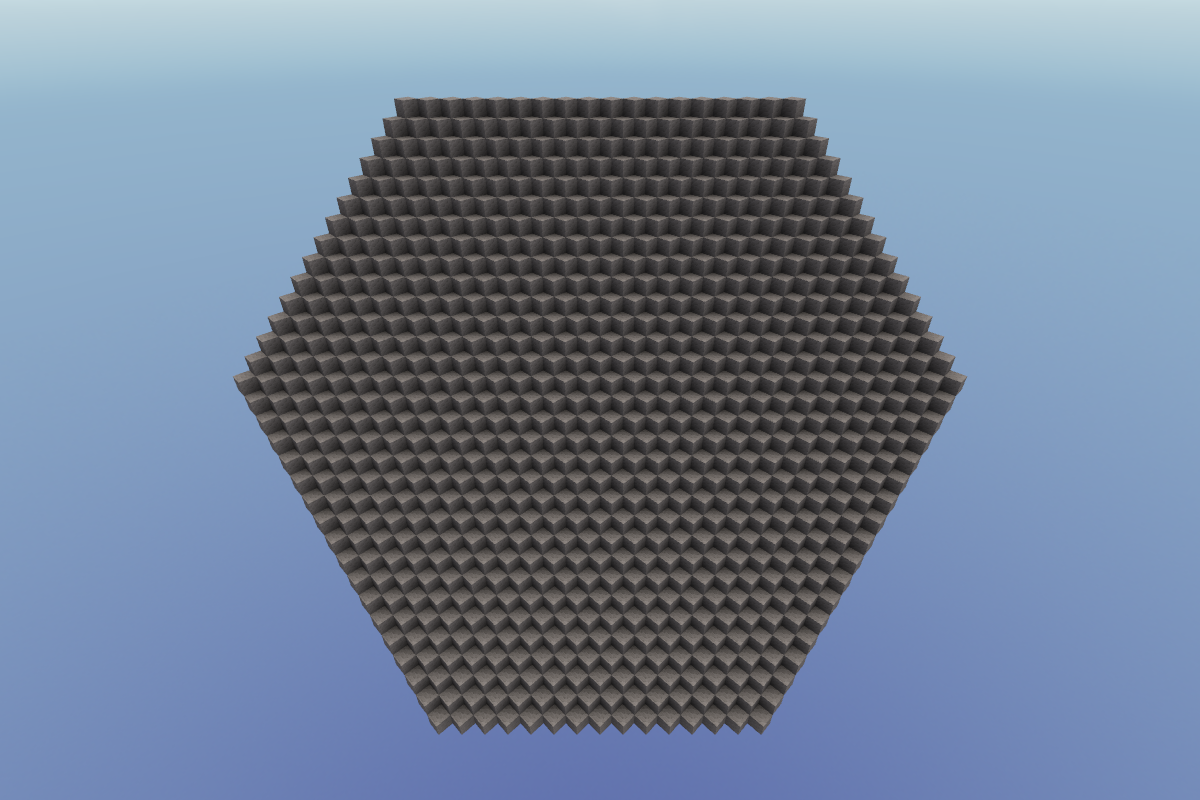
\includegraphics[width=.8\textwidth]{fps-hexagon.png}
	\caption{Screenshot der Blockformation in Szenario 1. Die Blöcke bilden ein stilisiertes Hexagon. Es ist \emph{nicht} gleichseitig. Die Formation ermöglicht den Blick auf je drei Seiten jedes Blocks und besteht aus 766 Blöcken.}\label{fig:hexagon}
\end{figure}
Die Anordnung der Blöcke in Szenario 1 ist in Abbildung~\ref{fig:hexagon} dargestellt. Wie auf der Abbildung bei genauem Hinsehen zu erkennen ist, sind von jedem Block drei Seiten sichtbar. Dadurch lässt sich die genaue Anzahl der Elemente bestimmen, die gezeichnet werden. Damit lässt sich die Gesamtzahl der gezeichneten Polygone\footnote{In der Blocklib besteht jedes gezeichnete Element aus Dreiecken oder aus Rechtecken, zusammenfassend werden diese als Polygone bezeichnet. Die meisten Elemente in der Welt werden als Dreiecke gezeichnet, die Elemente der graphischen Oberfläche nutzen Rechtecke. Jede Seite eines Blocks aus zwei Dreiecken hier aus zwei Dreiecken zusammengesetzt. Siehe dazu Auch Abbildung~\ref{fig:cube}.} für dieses Szenario genau berechnen. Jeden Frame müssen genau $766\cdot3\cdot2 + 3\cdot2-1 = 4596 +5 = 4601$ Polygone gezeichnet werden. Die $5$ zusätzlichen Polygone stammen von der \emph{Skybox}, einem großen Würfel um die Spielwelt herum, der eine Himmelstextur zeigt. Eines der Dreiecke der drei Seiten der Skybox ist außerhalb des Sichtfelds. Daher müssen nur $5$ Polygone hinzugezählt werden.

\begin{figure}[!htbp]
	\fpsplot{seed-0-hexagon}
	\caption{Seed 0 Hexagon}\label{fig:seed-0-hexagon-fps}
\end{figure}
\paragraph{\ac{fps}} Abbildung~\ref{fig:seed-0-hexagon-fps} zeigt den Verlauf der \si{\fps}. Die Framerate unter SystemA ist durchschnittlich \SI{337}{\fps} unter SystemB \SI{1133}{\fps}. Das ist ein Zuwachs von \SI{236}{\percent}. Unter SystemA ist der Start der Blocklib schneller. Hier werden Frames nach \SI{11,2}{\second} erzeugt, in SystemB nach \SI{13,6}{\second}. SystemB benötigt für den Start also \SI{21}{\percent} mehr Zeit. Über die Zeit hinweg bleiben die Frameraten beider Systeme in etwa konstant.


\begin{figure}[!htbp]
	\cpuplot{seed-0-hexagon}
	\caption{Seed 0 Hexagon}\label{fig:seed-0-hexagon-cpu}
\end{figure}
\paragraph{CPU} Der Verlauf der Auslastung der CPU durch die Blocklib ist in Abbildung~\ref{fig:seed-0-hexagon-cpu} zu sehen. Beide System zeigen hier eine Spitze in der Auslastung beim Start der Blocklib. In SystemA ist die maximale Auslastung von \SI{47}{\percent} nach \SI{11,6}{\second} erreicht, SystemB erreicht eine Auslastung von \SI{42}{\percent} nach \SI{15,6}{\second}. Die maximale Auslastung ist bei SystemB \SI{11}{\percent} niedriger als be SystemA. Die durchschnittliche Auslastung in der Hauptphase ist in SystemB mit einem Wert von \SI{18}{\percent} um \SI{38}{\percent} höher als in SystemB mit durchschnittlich \SI{13}{\percent}. Nach den anfänglichen Spitzen ist die Auslastung in beiden System in etwa konstant.

\begin{figure}[!htbp]
	\gpuplot{seed-0-hexagon}
	\caption{Seed 0 Hexagon}\label{fig:seed-0-hexagon-gpu}
\end{figure}
\paragraph{GPU} Der in Abbildung~\ref{fig:seed-0-hexagon-gpu} dargestellte Graph beschreibt die Auslastung der GPU im zeitlichen Verlauf. Da für diese Messungen ein externer Profiler genutzt wird, kann die Auslastung der GPU über die gesamte Messzeit hinweg ermittelt werden. Die Daten zu Beginn und zum Ende der Messung sind allerdings mit Vorsicht zu betrachten. So ist Auslastungsspitze zu Beginn der Messung nicht der Blocklib selbst zuzuordnen und zum Ende der Messung kann der Abfall der Auslastung nach Beendigung der Blocklib beobachtet werden. 

Da der GPU Profiler manuell gestartet werden muss, lassen sich die Auslastungswerte zu Beginn der Messung nicht gesichert vergleichen. Da der steile Abfall der Auslastung nach Beendigung der Blocklib bei beiden System gleichseitig ist, kann angenommen werden, dass zumindest grobe Trends zeitlich vergleichbar sind.

Auch in der Auslastung der GPU ist zu erkennen, dass der Start der Blocklib mit SystemA schneller ist als mit SystemB. Während in SystemA bereits nach \SI{7}{\second} eine Auslastungsspitze von \SI{27}{\percent} gemessen wird, ist der erste markante Anstieg der Auslastung (auf \SI{27}{\percent}) in SystemB  erst nach \SI{12}{\second} zu sehen. Die durchschnittliche Auslastung ist in beiden Systemen mit \SI{38}{\percent} in SystemA und \SI{36}{\percent} in SystemB fast identisch (Anstieg von \SI{1}{\percent} in SystemB). Während in SystemB nach \SI{20}{\second} und dem Abschluss der Startphase die Auslastung fast konstant knapp unter \SI{40}{\percent} liegt, oszilliert die Auslastung in SystemA lange zwischen \SI{30}{\percent} und \SI{40}{\percent}, bis sie schließlich nach etwa \SI{50}{\second} ebenfalls konstant bei knapp \SI{40}{\percent} liegt.

\begin{figure}[!htbp]
	\memplot{seed-0-hexagon-single-mem.csv}
	\memplot{seed-0-hexagon-multi-mem.csv}
	\caption{Seed 0 Hexagon}\label{fig:seed-0-hexagon-mem}
\end{figure} 
\paragraph{RAM} Betrachtet man den in Abbildung~\ref{fig:seed-0-hexagon-mem} gezeigten Vergleich der Speichernutzung zwischen SystemA und SystemB, lässt sich erkennen, dass SystemB sowohl während des Starts der Blocklib, als auch allgemein mehr Speicher benötigt, als SystemA. Der gelbe Bereich zeigt den von Java Insgesamt angeforderten Speicher. Zum Beginn ist das bei SystemB \SI{1730}{\mega\byte} und während des Großteils der Messung \SI{947}{\mega\byte}. SystemA benötigt die ersten \SI{37}{\second} \SI{644}{\mega\byte} Speicher, was sich bis zum Ende der Messung auf \SI{382}{\mega\byte} verringert. Durchschnittlich benötigt SystemB mit \SI{947}{\mega\byte} \SI{64}{\percent} mehr Speicher als SystemA mit durchschnittlich \SI{576}{\mega\byte} Speicherbedarf.

Der rote Bereich zeigt den Speicherverbrauch kurzlebiger Objekte an. In SystemB steigt die Menge der neu erzeugten Objekte deutlich schneller an als in SystemA. Damit einher geht auch die Anzahl der durchgeführten \emph{Garbage Collections}\footnote{Wird ein Objekt in Java nicht mehr gebraucht, kann der Speicher wieder freigegeben werden. Das passiert automatisch durch den sogenannten Garbage Collector. Dieser wird nicht immer sofort tätig sondern nur zu bestimmten Situationen, insbesondere dann, wenn die freie Speichermenge zuneige geht.}. Die Spitzen in den roten Graphen markieren Zeiten zu denen der Garbage Collector aktiv geworden ist. In SystemA gibt es über die gesamte Messzeit 13 Garbage Collections, in SystemB sind es 21. Damit lässt sich abschätzen, dass SystemB kontinuierlich etwa \SI{61}{\percent} schneller Speicher mit neu erzeugten, kurzlebigen Objekten belegt als SystemA. Hier ist allerdings nicht berücksichtigt, dass SystemB mehr Speicher belegt, und somit  weniger Garbage Collections, benötigt wenn die Erzeugungsraten gleich sind. Berechnet man die mittlere Steigung der positiven Anstiege des roten Graphen, kann man ermitteln wie viel Speicher pro Sekunde für die Erzeugung neuer Objekte genutzt wird. SystemA verbraucht \SI{70}{\mega\byte\per\second}, SystemB respektive \SI{274}{\mega\byte\per\second}. Das ist ein Anstieg von \SI{291}{\percent}, deutlich mehr, als die geschätzten \SI{61}{\percent}.
\subsubsection{Szenario 2: Halb-Würfel}
\begin{figure}
	\centering
	%\tikzset{external/remake next}
	\begin{tikzpicture}[spy using outlines={rectangle, red, magnification=6,
		size=3.8cm, connect spies}]
		\node{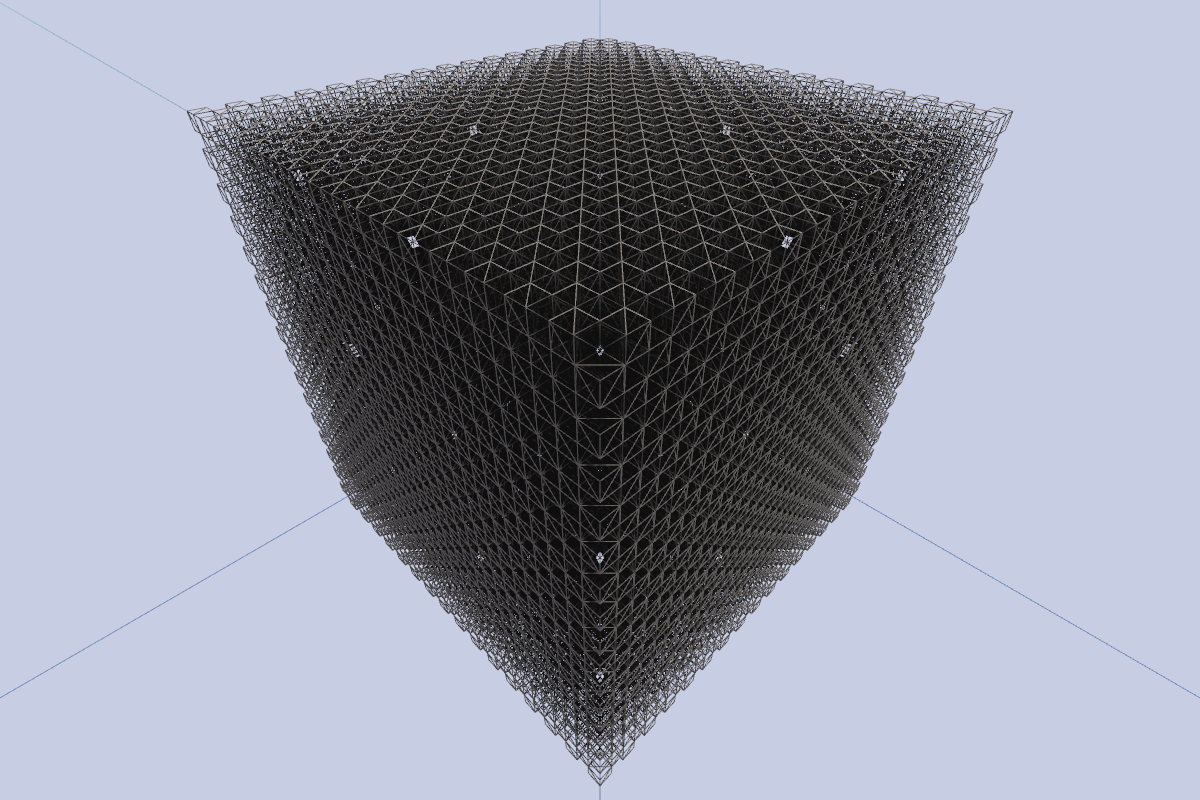
\includegraphics[width=.7\textwidth]{fps-cube.png}};
		\spy on (-3.8,2.65) in node [right] at (-10,2);
		\spy on (0.25,.65) in node [right] at (-10,-2);
	\end{tikzpicture} 
	\caption{Halbwürfel Bild}\label{fig:cube}
\end{figure}
Da die Anzahl der zu zeichnenden Objekte in dem ersten Szenario relativ gering ist, wird diese in Szenario 2, das in Abbildung~\vref{fig:cube} veranschaulicht ist, erhöht. In diesem Szenario wird ein Bereich von $32 \times 32 \times 32$ Blöcken so befüllt, dass an jeder zweiten Stelle ein Block ist. Zweidimensional entspricht das einem Schachbrettmuster. Die Anzahl der platzierten Blöcke ist damit $\frac{1}{2}\cdot32^3 = 16384$. Die Anzahl der zu zeichnenden Dreiecke ist $16384\cdot6 + 5 = 98309$.

Aufgrund der Anordnung wären allerdings nur wenige Blöcke sichtbar. Daher wird das Drahtgittermodell gezeichnet, also nur die Kanten der zu zeichnenden Dreiecke. Dennoch kann hier nicht mehr sichergestellt werden, dass auch tatsächlich alle Elemente gezeichnet werden, da selbst mit dem Drahtgittermodell an vielen Stellen Polygone überdeckt werden. Durch die Darstellung als Drahtgittermodell lassen sich nun auch die Kanten der Skybox erkennen und man sieht, dass das Dreiecke in der oberen rechten Ecke nicht gezeichnet wird. 

\begin{figure}[!htb]
	\fpsplot{seed-0-cube}
	\caption{Seed 0 Halb-Würfel}\label{fig:seed-0-cube-fps}
\end{figure}
\paragraph{\ac{fps}}Der Verlauf der Framerate für Szenario 2 ist in Abbildung~\vref{fig:seed-0-cube-fps} dargestellt. In SystemA werden Frames ab Sekunde $11$ erzeugt, in SystemB ab Sekunde $13$. Die mittlere Framerate in SystemA ist \SI{253}{\fps} und in SystemB \SI{417}{\fps}. Damit erhöht sich die Framerate in SystemB um \SI{65}{\percent}. Dieser Wert ist deutlich geringer als in Szenario 1. Die Frameraten bleiben in beiden Systemen sehr konstant.

\begin{figure}[!htb]
	\cpuplot{seed-0-cube}
	\caption{Seed 0 Halb-Würfel}\label{fig:seed-0-cube-cpu}
\end{figure}
\paragraph{\ac{cpu}} Die Auslastung der \ac{cpu} in Szenario 2, zu sehen in Abbildung~\vref{fig:seed-0-cube-cpu}, gestaltet sich vergleichbar zu der in Szenario 1. Die Mittelwerte sind mit \SI{13}{\percent} in SystemA und \SI{18}{\percent} in SystemB nach Rundung identisch zu Szenario 1.
Auffällig ist, dass SystemB wie in Szenario 1 in den ersten Sekunden, während des Starts der Blocklib, zwei Auslastungsspitzen besitzt (\SI{32}{\percent} und \SI{50}{\percent}). SystemA dagegen besitzt nur eine (\SI{46}{\percent}). Eine mögliche Erklärung dafür ist die Trennung von Simulation und Rendering in verschiedene Threads. Dadurch könnte es passieren, die \ac{cpu} zeitweise dadurch entlastet ist, dass die \ac{gpu} Zeit benötigt, um übergebene \glspl{Anweisung} auszuführen, beispielsweise wenn Texturen zum Start auf die \ac{gpu} geladen werden.

\begin{figure}[!htb]
	\gpuplot{seed-0-cube}
	\caption{Seed 0 Halb-Würfel}\label{fig:seed-0-cube-gpu}
\end{figure}
\paragraph{\ac{gpu}} Die \ac{gpu}-Auslastung des Halb-Würfel Szenario unterscheidet sich im Gegensatz zur \ac{cpu}-Auslastung sehr von der im Hexagon-Szenario gemessenen. In Abbildung~\vref{fig:seed-0-cube-gpu} ist die gemessene \ac{gpu}-Auslastung zeitlich aufgetragen. Anders als in Szenario 1 ist in beiden Systemen der Unterschied in der Auslastung unübersehbar. SystemB nutzt nach dem Start durchschnittlich \SI{94}{\percent} der Leistung der \ac{gpu}, während SystemA nur \SI{60}{\percent} Auslastung erzeugt. Über die gesamte Messdauer liegt SystemB damit bei \SI{70}{\percent} Auslastung und SystemA bei \SI{45}{\percent}. Betrachtet man nur die Auslastung nach dem Start lässt sich eine Steigerung der Auslastung um \SI{57}{\percent} errechnen.

\begin{figure}[!htb]
	\memplot{seed-0-cube-single-mem.csv}
	\memplot{seed-0-cube-multi-mem.csv}
	\caption{Seed 0 Halb-Würfel}\label{fig:seed-0-cube-mem}
\end{figure} 
\paragraph{\ac{ram}} Die Speichernutzung in Szenario 2 wird in Abbildung~\vref{fig:seed-0-cube-mem} gezeigt. Der Ge\-samt-Spei\-cher\-ver\-brauch von SystemA steigt im Vergleich zum Hexagon-Szenario leicht während der Speicherverbrauch von SystemB beinahe identisch bleibt. SystemA benötigt durchschnittlich \SI{643}{\mega\byte} und SystemB \SI{941}{\mega\byte}. Das ist ein Anstieg von \SI{12}{\percent} in SystemA und eine leichte Verringerung um \SI{1}{\percent} in SystemB. Weiterhin zeigt SystemB einen großen Speicherverbrauch während des Starts der Blocklib (\SI{1732}{\mega\byte}).

Die Speichernutzung der kurzlebigen Objekte ist sowohl in SystemA mit \SI{53}{\mega\byte\per\second} als auch in SystemB mit \SI{101}{\mega\byte\per\second} niedriger als in Szenario 1. Insbesondere SystemB verbraucht mit neu erzeugten Objekten weniger als halb so viel Speicher. Vergleicht man die beiden Systeme in diesem Szenario erhält man einen Anstieg von \SI{91}{\percent} Speicherverbrauch mit SystemB. Der geringere Speicherverbrauch führt auch zu einer geringeren Anzahl an Garbage Collections. Da SystemB allgemein mehr Speicher nutzt als SystemA ist die Anzahl der Garbage Collections im gemessenen Zeitraum in SystemB mit 10 Collections um eins niedriger als in SystemA. Der zusätzliche Speicher gleicht also den höheren dauerhaften Speicherverbrauch aus. 

Der langlebige Speicherverbrauch bleibt in beiden Systemen mit \SI{296}{\mega\byte} (SystemA) und \SI{320}{\mega\byte} (SystemB) sehr konstant. In SystemA sinkt der Speicherverbrauch, wie auch schon im Hexagon-Szenario zu beobachten, nach etwa \SI{45}{\second} auf zum Ende hin nur noch \SI{129}{\mega\byte}.
\subsubsection{Szenario 3: Welt-Statisch}
Neben den beiden selbst erzeugten Szenarien, werden nun Szenarien betrachtet, in denen die Terrain-Generierung der Blocklib genutzt wird. Für die Generierung nutzt die Blocklib einen Pseudo-Zufallszahlengenerator. Das ist ein Algorithmus, der ausgehend von einem übergebenen Wert, dem sogenannten \emph{Seed} Werte erzeugt, die zufällig \emph{wirken}. Der Algorithmus ist allerdings deterministisch. Mit demselben Seed wird immer dieselbe Folge von Zahlen generiert.

\begin{figure}
	\centering
	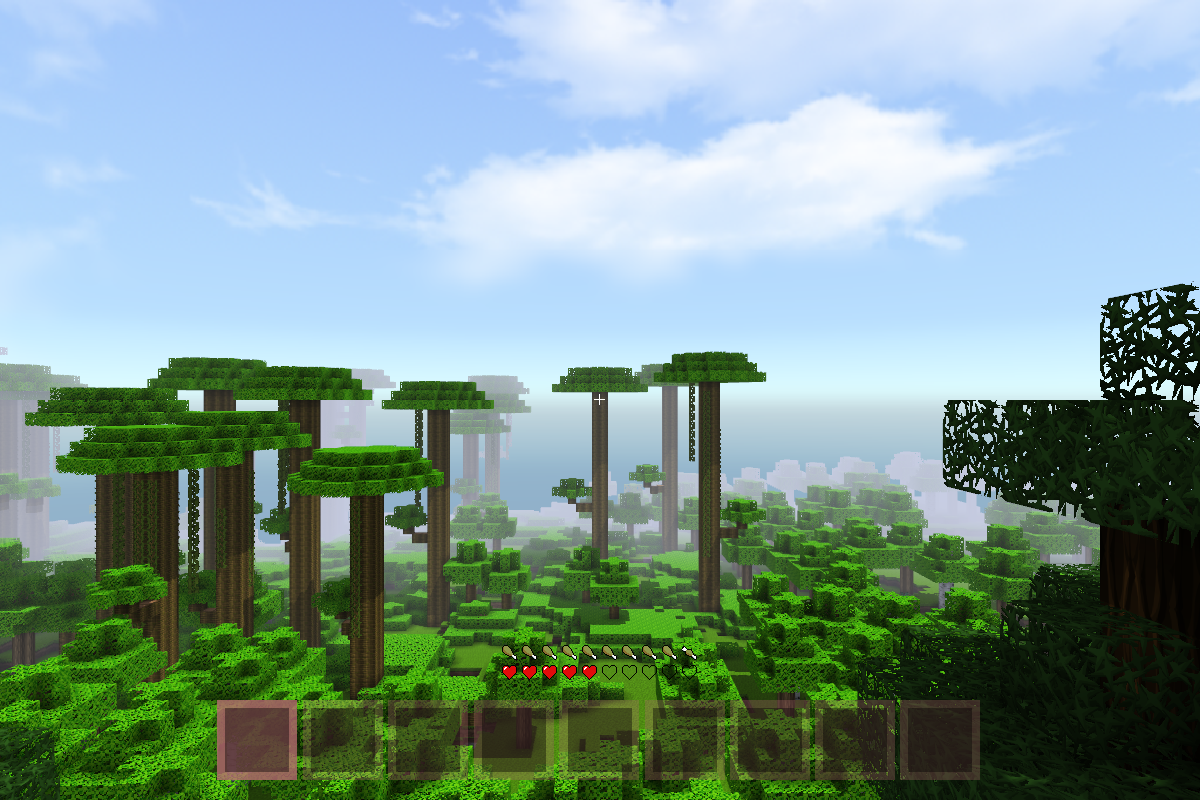
\includegraphics[width=.49\textwidth]{seed-0.png}
	\hfill
	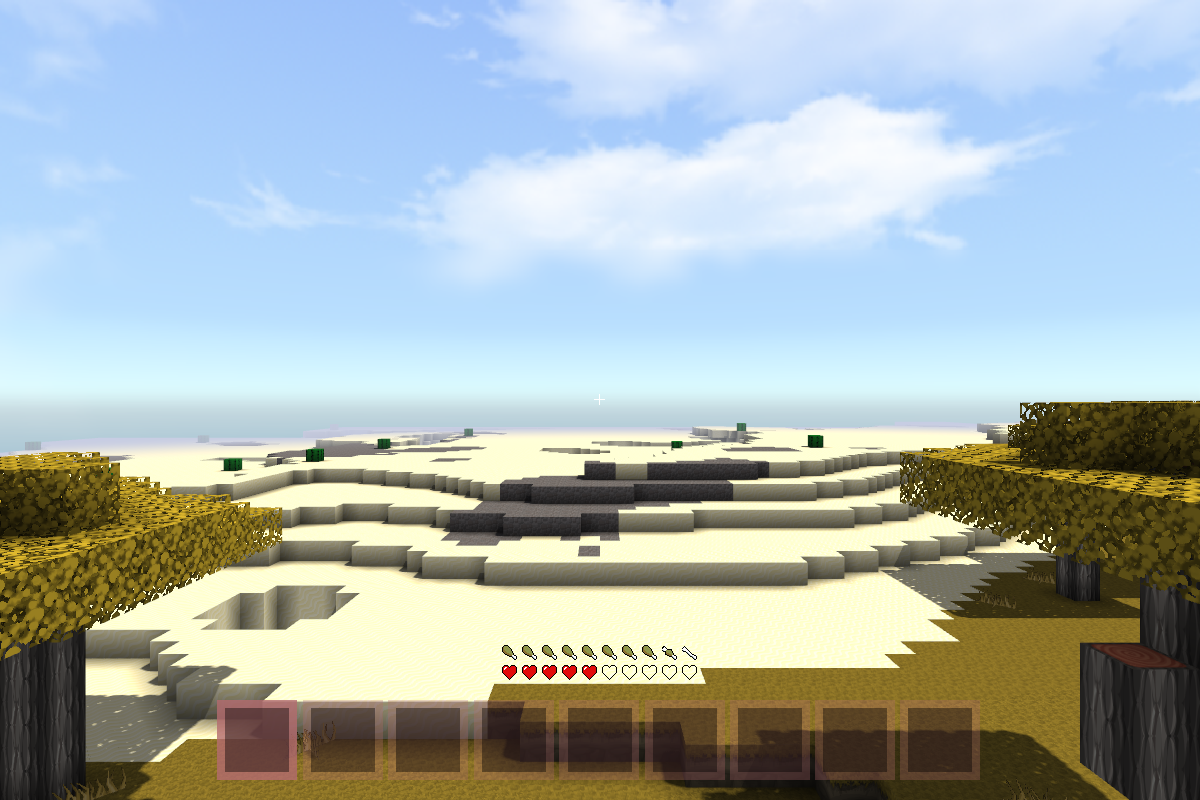
\includegraphics[width=.49\textwidth]{seed-2.png}
	\caption[Darstellungen von mit der Terrain-Generierung der Blocklib erzeugten Welten mit unterschiedlichen Seeds.]{Darstellungen von mit der Terrain-Generierung der Blocklib erzeugten Welten mit unterschiedlichen Seeds. Links wird der Seed 0 verwendet, rechts der Seed 2. Durch diese kleine Änderung entstehen völlig andere Welten.}\label{fig:static}
\end{figure}
Damit SystemA und SystemB bei Messungen mit Terrain-Generierung vergleichbar sind, wird in beiden Systemen derselbe Seed verwendet, wodurch dieselbe Welt generiert wird. Abbildung~\ref{fig:static} zeigt zwei Screenshots von generierten Welten. Das linke Bild zeigt die mit dem Seed $0$ generierte Welt, das rechte Bild nutzt als Seed $2$. Hier sieht man beispielhaft, dass bereits kleine Unterschiede im Seed völlig andere Welten erzeugen. Für die folgenden Messungen wird der Seed $0$ verwendet. 

Im Szenario Welt-Statisch bleibt die Kamera wie in den vorherigen beiden Szenarien an ein und derselben Stelle.



\paragraph{\ac{fps}}
\begin{figure}[!htbp]
	\fpsplot{seed-0-static}
	\caption{Graph des Verlaufs der Framerate in Szenario 3: Welt-Statisch.}\label{fig:seed-0-static-fps}
\end{figure}
Der Verlauf der \ac{fps} in diesem Szenario ist in Abbildung~\ref{fig:seed-0-static-fps} abgebildet. Vergleicht man die Framerate mit denen der vorherigen Szenarien, lässt sich erkennen, dass die Startphase sich in beiden Systemen verlängert. SystemA benötigt \SI{20}{\second} statt \SI{15}{\second}, um eine konstante Framerate von etwa \SI{201}{\fps} zu erreichen. SystemB erreicht einen stabilen Zustand nach etwa \SI{22}{\second} mit durchschnittlich \SI{468}{\fps}.
Beide Systeme benötigen mit Terrain-Generierung also etwa \SI{5}{\second} länger für den Start. SystemB erreicht nach dem Start eine um \SI{133}{\percent} gesteigerte Framerate gegenüber SystemA. Dieser Wert liegt zwischen den gemessenen Werten der ersten beiden Szenarien. Des Weiteren ist liegt die Bildwiederholrate von SystemA in diesem Szenario unter der in Szenario 2 gemessenen, während sie in SystemB höher liegt.

\paragraph{\ac{cpu}}
Unter Betrachtung der \ac{cpu}-Auslastung im Welt-Statisch Szenario, die in Abbildung~\ref{fig:seed-0-static-cpu} zu sehen ist, lässt sich der zusätzliche Aufwand für die Terrain-Generierung der Welt ebenfalls erkennen.
\begin{figure}[!htbp]
	\cpuplot{seed-0-static}
	\caption[Graph des Verlaufs der \glsentryshort{cpu}-Auslastung in Szenario 3: Welt-Statisch.]{Graph des Verlaufs der \ac{cpu}-Auslastung in Szenario 3: Welt-Statisch.}\label{fig:seed-0-static-cpu}
\end{figure}
Während des Starts der Blocklib lasten beide Systeme die \ac{cpu} bis zu \SI{97}{\percent} aus. Nach dem Start fällt die Auslastung in beiden Systemen, auf durchschnittlich \SI{13}{\percent} in SystemA und \SI{23}{\percent} in SystemB.
SystemB führt im Vergleich zu SystemA in diesem Szenario also zu einer um \SI{77}{\percent} erhöhten Auslastung der \ac{cpu}. SystemB lastet die \ac{cpu} in diesem Szenario mehr aus als in den Szenarien ohne generierte Welt. SystemA dagegen erreicht nach dem Start eine zu den bisherigen Szenarien vergleichbare Auslastung.

\paragraph{\ac{gpu}}
Der zeitliche Verlauf der \ac{gpu}-Auslastung von Szenario 3 ist in Abbildung~\ref{fig:seed-0-static-gpu} zu sehen. Die durchschnittliche Auslastung der \ac{gpu} liegt in SystemA bei \SI{40}{\percent} und in SystemB bei \SI{71}{\percent}. Die Auslastung in SystemA entspricht damit der aus dem Hexagon Szenario. SystemB dagegen erreicht eine deutlich höhere Auslastung. In beiden Systemen ist die \ac{gpu} noch nicht vollständig ausgelastet. Wie auch schon in den anderen Messungen zu Szenario 3 zu erkennen ist, zeigt die erst später ansteigende Auslastung der \ac{gpu} eine länger dauernde Startphase an. Die Auslastung beider Systeme bleibt während der Hauptphase weitgehend konstant.
\begin{figure}[!htbp]
	\gpuplot{seed-0-static}
	\caption[Graph des Verlaufs der \glsentryshort{gpu}-Auslastung in Szenario 3: Welt-Statisch.]{Graph des Verlaufs der \ac{gpu}-Auslastung in Szenario 3: Welt-Statisch.}\label{fig:seed-0-static-gpu}
\end{figure}

\paragraph{\ac{ram}}
Die Speichernutzung im Welt-Statisch Szenario ist in beiden Systemen höher als in den vorherigen Szenarien. Abbildung~\ref{fig:seed-0-static-mem} beschreibt deren Verlauf. 
\begin{figure}[!htbp]
	\memplot[xticklabels={,,},xlabel={}]{seed-0-static-single-mem.csv}
	\\\memplot{seed-0-static-multi-mem.csv}
	\caption{Graph des Verlaufs der Speichernutzung in Szenario 3: Welt-Statisch.}\label{fig:seed-0-static-mem}
\end{figure} 
Wie in Szenario 2 ist die Geschwindigkeit, mit der Speicher für die Erzeugung kurzlebiger Objekte verbraucht wird, in SystemB mit \SI{208}{\mega\byte\per\second} etwa doppelt so hoch wie in SystemA mit \SI{94}{\mega\byte\per\second}. Allerdings ist die Geschwindigkeit beider Systeme damit in Szenario 3 wiederum etwa doppelt so hoch wie im Halb-Würfel Szenario.
Auch der Gesamtverbrauch \ac{ram} ist in beiden Systemen etwa doppelt so groß. SystemA nutzt während der Hauptphase \SI{1243}{\mega\byte} und SystemB \SI{1793}{\mega\byte}. SystemB nutzt in diesem Szenario also \SI{44}{\percent} mehr Speicher als SystemA.   
%\subsubsection{Szenario 4: Welt-Rotation}
%Die bisherigen Szenarien nutzen eine statische Kamera. Das erlaubt zwar konstante Messungen, entspricht allerdings keiner realistischen Situation. Normalerweise wird die Kamera bewegt und rotiert. Die folgenden Szenarien stellen dynamische Situationen dar, in denen die Kamera bewegt wird. In diesem Szenario wird die Kamera dauerhaft rotiert mit einer Winkelgeschwindigkeit von \SI{45}{\degree\per\second}. Eine Reihe von Screenshots, die die Rotation zeigt, ist in Abbildung~\ref{fig:rotate} zu sehen.
\begin{figure}
	\centering
	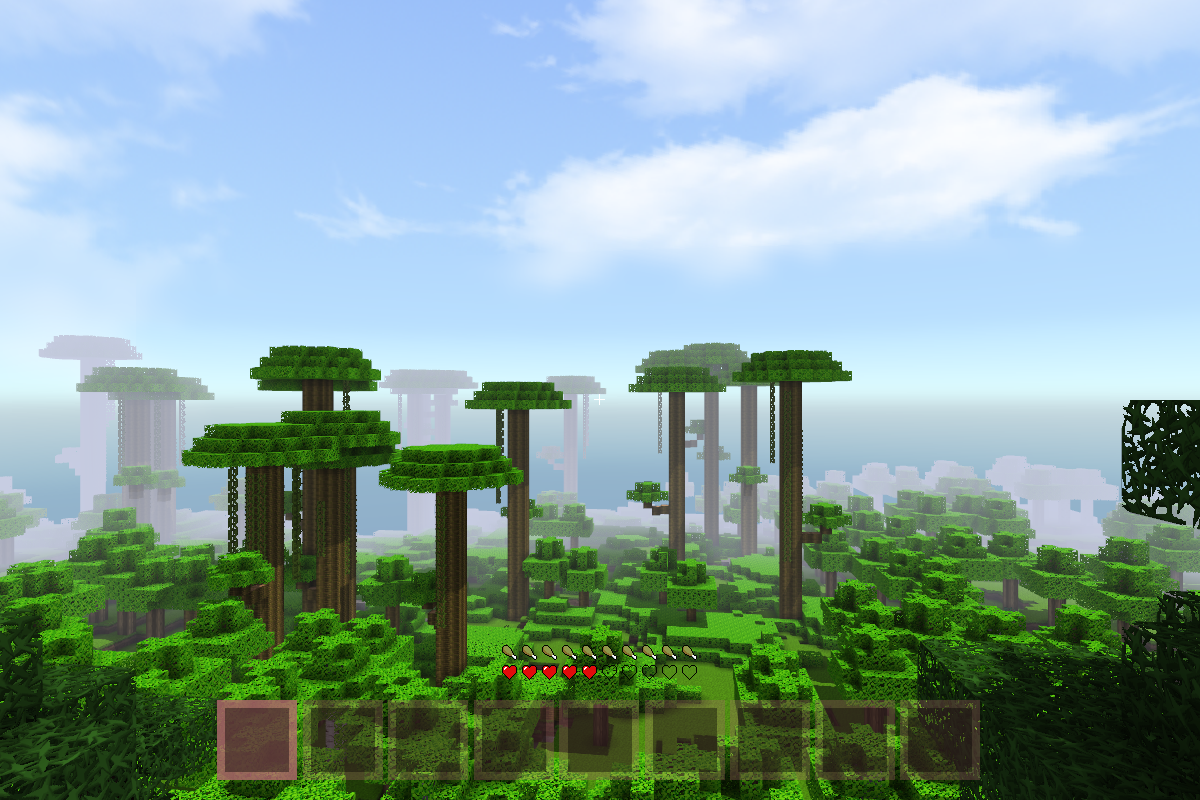
\includegraphics[width=.32\textwidth]{rotate-1.png}
	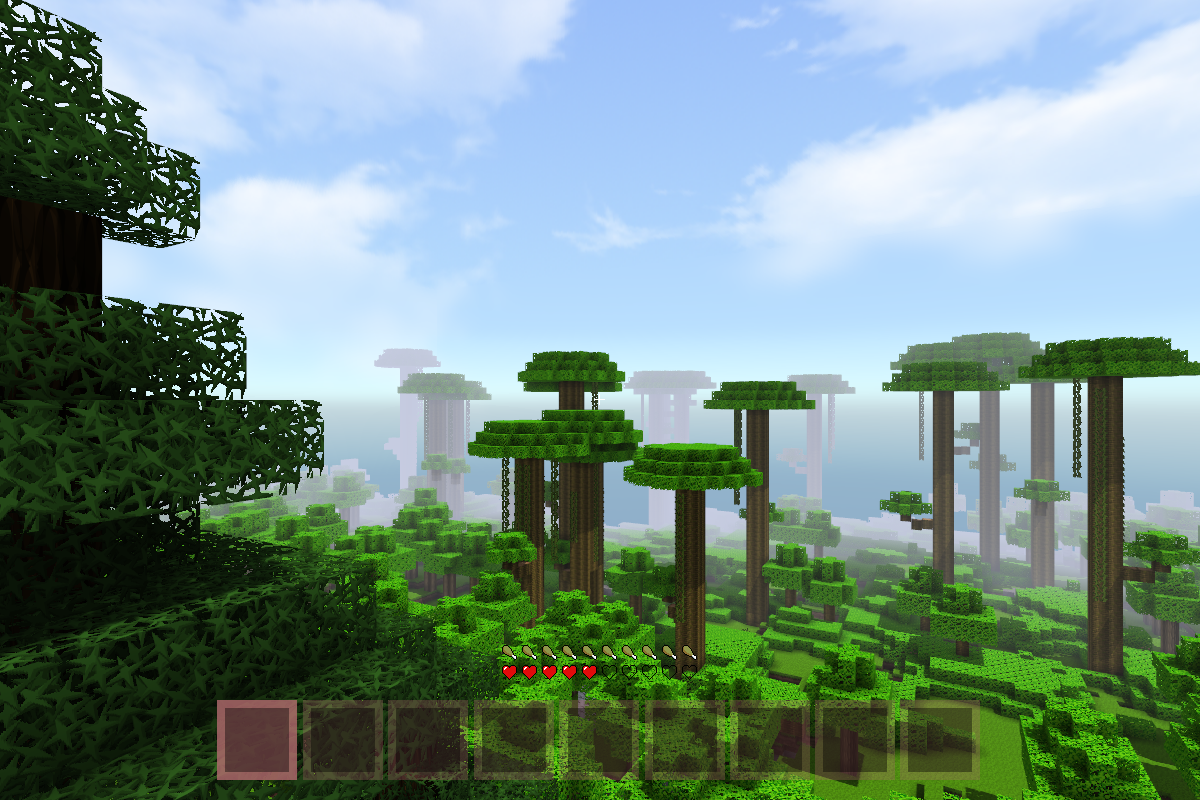
\includegraphics[width=.32\textwidth]{rotate-2.png}
	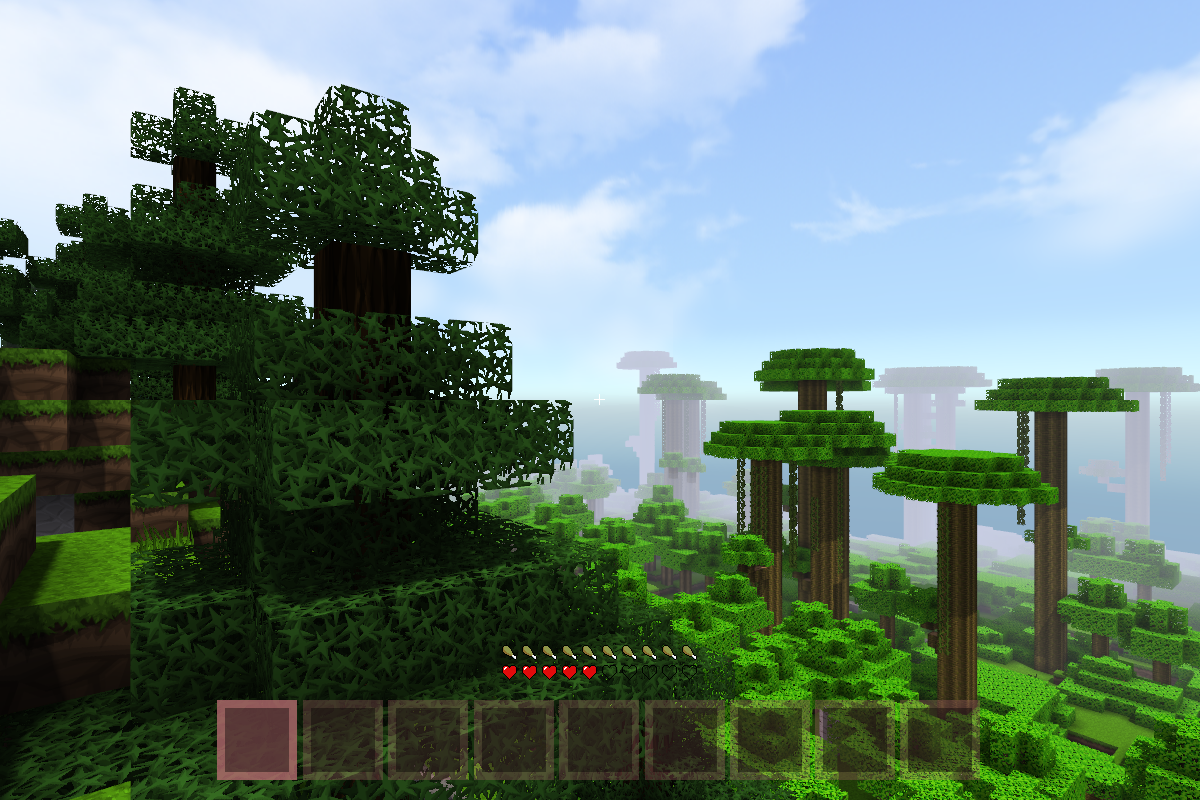
\includegraphics[width=.32\textwidth]{rotate-3.png}\\[4pt]
	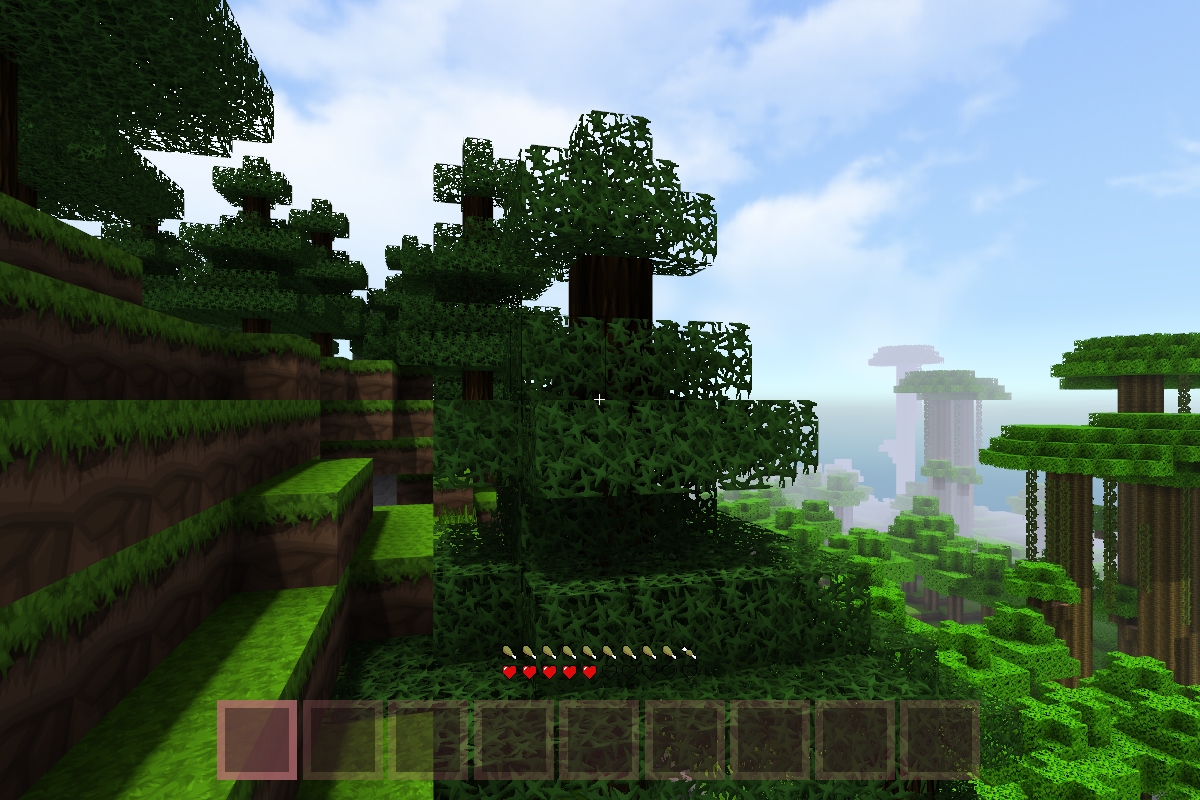
\includegraphics[width=.32\textwidth]{rotate-4.png}
	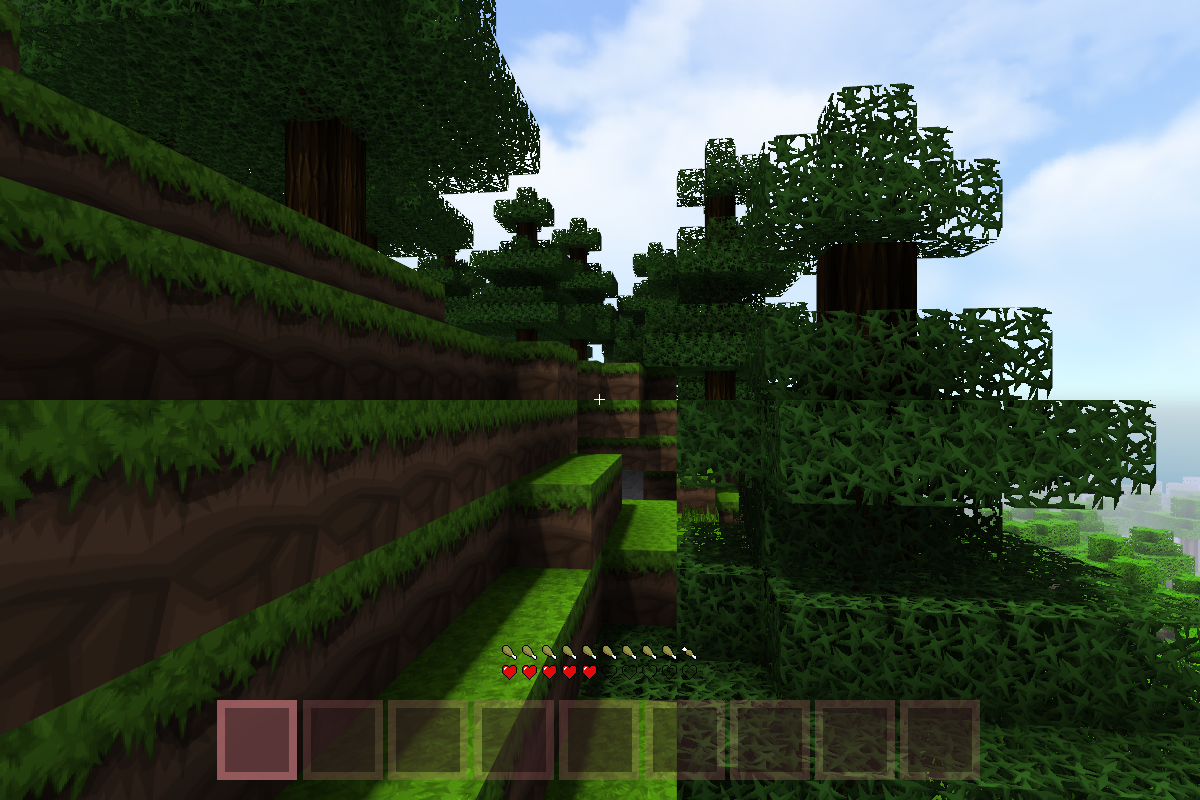
\includegraphics[width=.32\textwidth]{rotate-5.png}
	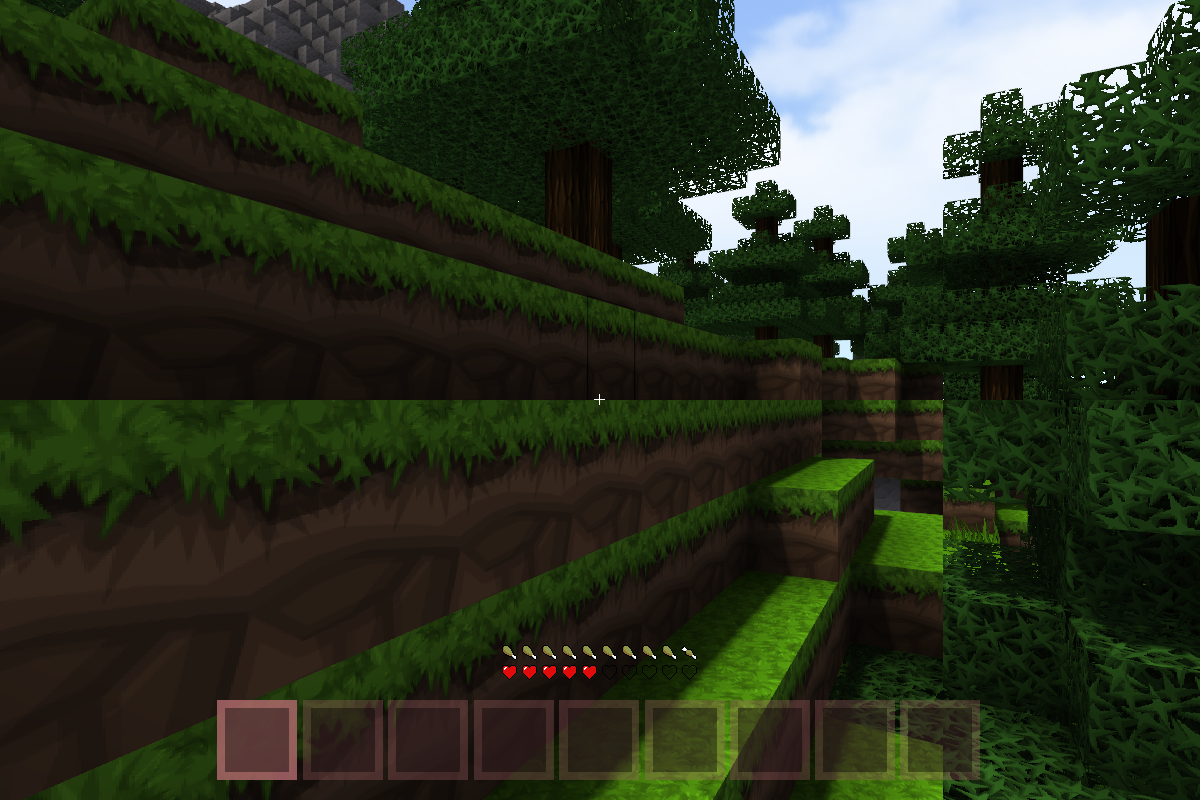
\includegraphics[width=.32\textwidth]{rotate-6.png}
	%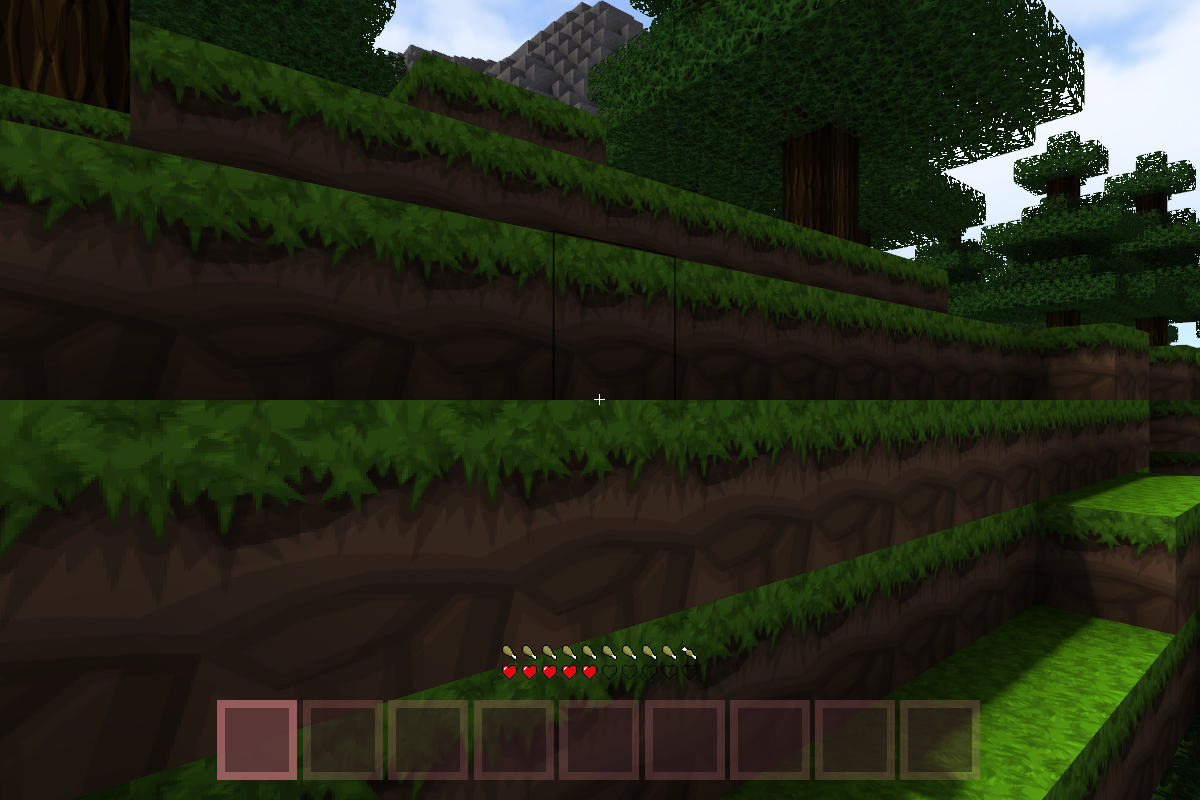
\includegraphics[width=.24\textwidth]{rotate-7.png}
	%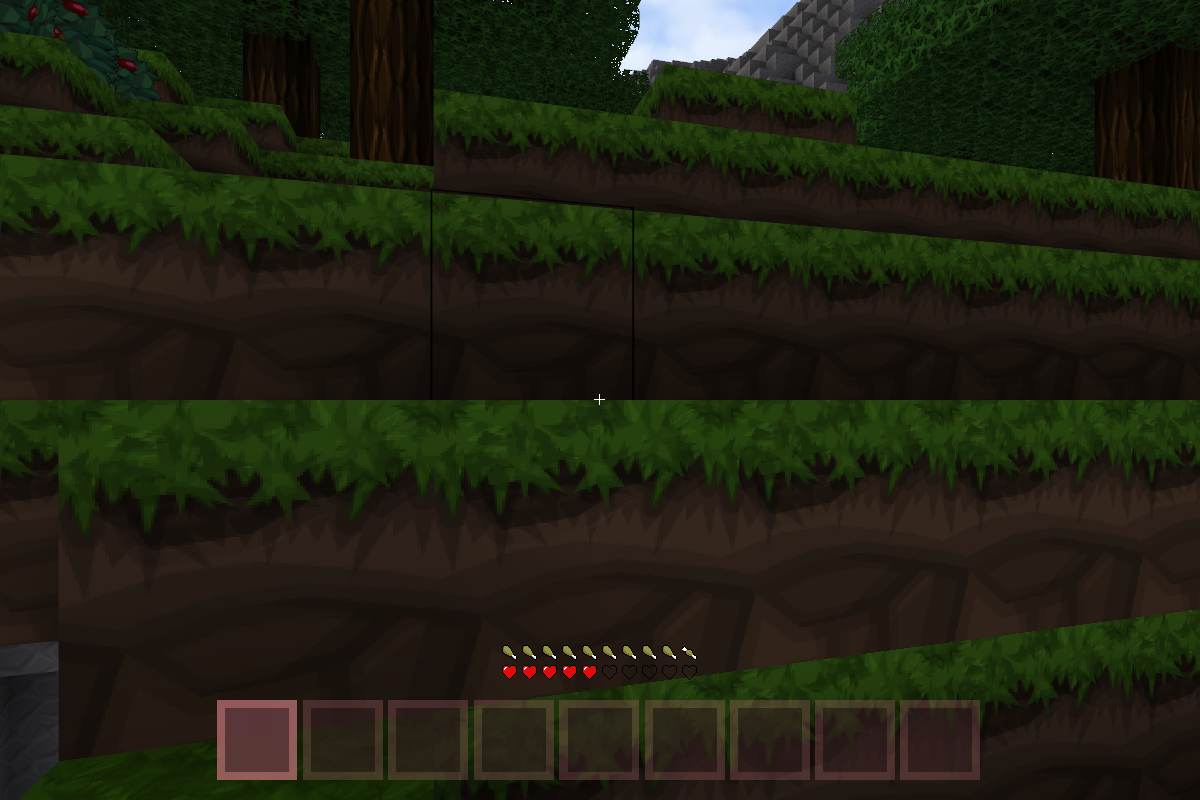
\includegraphics[width=.24\textwidth]{rotate-8.png}
	\caption{Reihe von Screenshots, die die Rotation in Szenario 4 zeigt. Die Rotationsrichtung ist gegen den Uhrzeigersinn. Die Screenshots haben einen Zeitabstand von \SI{500}{\milli\second}.}\label{fig:rotate}
\end{figure}
Wie an den Screenshots zu erkennen ist, wird auch für dieses Szenario der Seed 0 genutzt.

\paragraph{\ac{fps}}
Betrachtet man den Verlauf der \ac{fps} in diesem Szenario ergibt sich ein zu den vorherigen Szenarien sehr verschiedenes Muster. Zu sehen ist das in Abbildung~\ref{fig:seed-0-rotate-fps}.
\begin{figure}[!htbp]
	\fpsplot{seed-0-rotate}
	\caption{Graph des Verlaufs der Framerate in Szenario 4: Welt-Rotation.}\label{fig:seed-0-rotate-fps}
\end{figure}
 Zwar ist wieder zu erkennen, dass SystemB ein paar Sekunden später mit der Erzeugung von Bildern beginnt, das Verhalten der Framerate über die Zeit ist danach aber in den Szenarien einzigartig. In SystemA und viel mehr noch in SystemB ist eine zyklische Schwankung der \ac{fps} zu erkennen. Die Periode der Schwankungen beträgt in beiden Systemen \SI{8}{\second}. Das entspricht exakt der Periode der Rotation ($8\cdot45 = 360$). Unter Betrachtung der Screenshots in Abbildung~\ref{fig:rotate} lässt sich eine Hypothese aufstellen, woher diese Schwankungen kommen. In Seed 0 startet der Spielercharakter in der Nähe eines Berges. Ist die Kamera dem Tal zugewandt, müssen deutlich mehr Elemente gezeichnet werden als, wenn die Kamera dem Berg zugewandt ist. Durch die Rotation ändert sich also die Arbeitslast für die \ac{gpu} periodisch.

Durchschnittlich steigt die Bildwiederholrate von \SI{134}{\fps} in SystemA auf \SI{378}{\fps} in SystemB. Das ist eine Steigerung von \SI{182}{\percent}. In beiden System ist die Framerate geringer als im Szenario Welt-Statisch. Der Anstieg der Framerate von SystemA zu SystemB ist allerdings höher. SystemA erreicht ein Maximum von \SI{152}{\fps} und ein Minimum von \SI{113}{\fps}, ein Unterschied von \SI{39}{\fps}. SystemB erreicht maximal \SI{474}{\fps} und singt auf bis zu \SI{287}{\fps}, das ist eine Schwankung von \SI{187}{\fps}.

\paragraph{\ac{cpu}}
Im Gegensatz zu der Bildwiederholrate ist in der Auslastung der \ac{cpu} beinahe keine Schwankung zu erkennen. Insbesondere ist keine Periode von \SI{8}{\second} zu erkennen, wie Abbildung~\ref{fig:seed-0-rotate-cpu} erkennen lässt.
\begin{figure}[!htbp]
	\cpuplot{seed-0-rotate}
	\caption[Graph des Verlaufs der \glsentryshort{cpu}-Auslastung in Szenario 4: Welt-Rotation.]{Graph des Verlaufs der \ac{cpu}-Auslastung in Szenario 3: Welt-Statisch.}\label{fig:seed-0-rotate-cpu}
\end{figure}
Tatsächlich ist der Graph \ac{cpu}-Auslastung beinahe nicht von dem in Szenario 3 zu unterscheiden, mit der Ausnahme der Startphase. Hier sinkt die Auslastung der \ac{cpu} zum ersten Mal in SystemB zuerst. Die durchschnittliche Auslastung der System ist allerdings identisch zum Welt-Statisch Szenario, \SI{13}{\percent} in SystemA und \SI{23}{\percent} in SystemB.

Die Tatsache, dass die Auslastungsmessung in SystemB zwei Sekunden früher endet, als in SystemA, ist ein Indiz dafür, dass die Messungen aus irgend einem Grund zeitlich verschoben sind. Das würde auch erklären, warum die Startphase in der \ac{cpu}-Auslastung zum ersten Mal in SystemB schneller vorbei ist als in SystemA. Zusätzlich ist die Startphase in der Messung der \ac{fps} in Gegensatz dazu weiterhin mit den vorherigen Szenarien konsistent. 

\paragraph{\ac{gpu}}
Auch der Auslastungsgraph der \ac{gpu} (siehe Abbildung~\ref{fig:seed-0-rotate-gpu}) unterstützt diese Hypothese. Hier ist wieder eine längere Startphase von einigen Sekunden in SystemB zu erkennen. Weiter lässt sich die Aussage scheinbar festigen, dass die Schwankungen der Framerate mit der Auslastung der \ac{gpu} zusammenhängen. Auch hier lässt sich eine achtsekündliche periodische Schwankung erkennen.
\begin{figure}[!htbp]
	\gpuplot{seed-0-rotate}
	\caption[Graph des Verlaufs der \glsentryshort{gpu}-Auslastung in Szenario 4: Welt-Rotation.]{Graph des Verlaufs der \ac{gpu}-Auslastung in Szenario 3: Welt-Statisch.}\label{fig:seed-0-rotate-gpu}
\end{figure}
Die Tatsache, dass diese Schwankung in SystemA wie bei der Framerate kleiner ist, als in SystemB, führt allerdings zu einer anderen Vermutung. Die Framerate und die \ac{gpu} hängen von der Belastung des Simulations-Threads ab. Die \ac{cpu} des Testsystems besitzt acht Hardware-Threads. Die Auslastung der \ac{cpu} liegt in allen bisherigen Szenarien in SystemA bei \SI{13}{\percent} was in etwa $\frac{1}{8}$ entspricht. Das legt zusammen mit der Tatsache, dass die Auslastung der \ac{gpu} immer unter \SI{100}{\percent} liegt, einen \ac{cpu}-Flaschenhals bezogen auf die Performance nahe. Diese These wird weiter dadurch unterstützt, dass die Verläufe von \ac{fps} und \ac{gpu}-Auslastung deckungsgleich und nicht gegengleich sind. Wäre die höhere Auslastung der \ac{gpu} für eine geringere Bildwiederholrate verantwortlich, müsste das genau anders herum sein.

Diese These ließe sich weiter untersuchen, indem die Auslastung der einzelnen Hardware-Threads gemessen wird. Diese Messung lässt sich in dieser Arbeit leider nicht mehr durchführen. 

Durchschnittlich liegt die Auslastung der \ac{gpu} in SystemA bei \SI{37}{\percent} und in SystemB bei \SI{53}{\percent}. Das ist ein Anstieg von \SI{43}{\percent}.

\paragraph{\ac{ram}}
Die Nutzung des Hauptspeichers, zu sehen in Abbildung~\ref{fig:seed-0-rotate-mem}, ist in Szenario Welt-Rotation grob vergleichbar mit Szenario Welt-Statisch.
\begin{figure}[!htbp]
	\memplot[xticklabels={,,},xlabel={}]{seed-0-rotate-single-mem.csv}
	\\\memplot{seed-0-rotate-multi-mem.csv}
	\caption{Graph des Verlaufs der Speichernutzung in Szenario 4: Welt-Rotation.}\label{fig:seed-0-rotate-mem}	
\end{figure} 
SystemA nutzt mit durchschnittlich \SI{1267}{\mega\byte} etwas mehr Speicher, SystemB mit \SI{1441}{\mega\byte} aber weniger. Somit ergibt sich in diesem Szenario ein Anstieg von \SI{14}{\percent} statt \SI{44}{\percent}. 

derselbe Trend lässt sich im kurzweiligen Verbrauch von Speicher erkennen. SystemA hat einen Verbrauch von durchschnittlich \SI{101}{\mega\byte\per\second} und SystemB nutzt \SI{187}{\mega\byte\per\second} was einen Anstieg von \SI{85}{\percent} bedeutet.

%\subsubsection{Szenario 5: Welt-Gehen}
%Das letzte Szenario ist das einzige, in dem nicht nur in der Startphase neue Chunks geladen werden. In Szenario 5: Welt-Gehen bewegt sich die Kamera in einer Welt mit Terrain-Generierung konstant in Blickrichtung nach vorne, wie in den Screenshots in Abbildung~\ref{fig:walk} zu sehen ist.
\begin{figure}[!htbp]
	\centering
	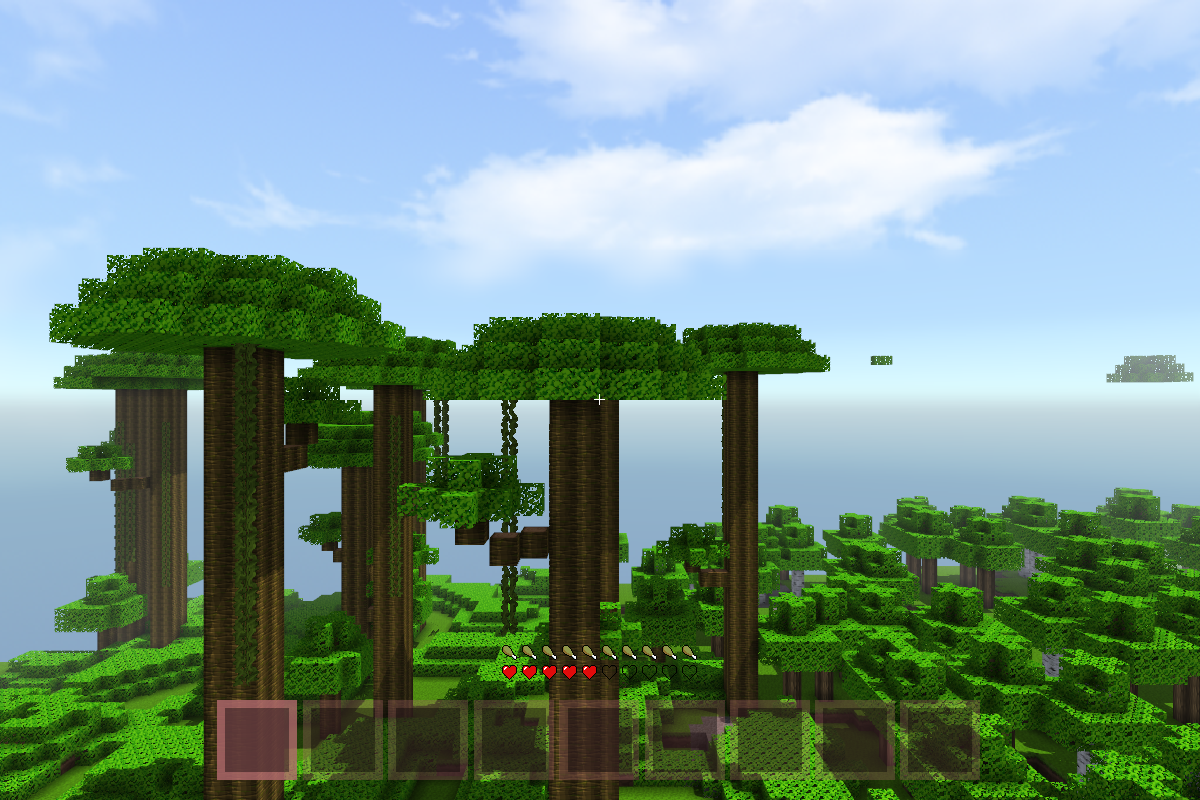
\includegraphics[width=.32\textwidth]{walk-1.png}
	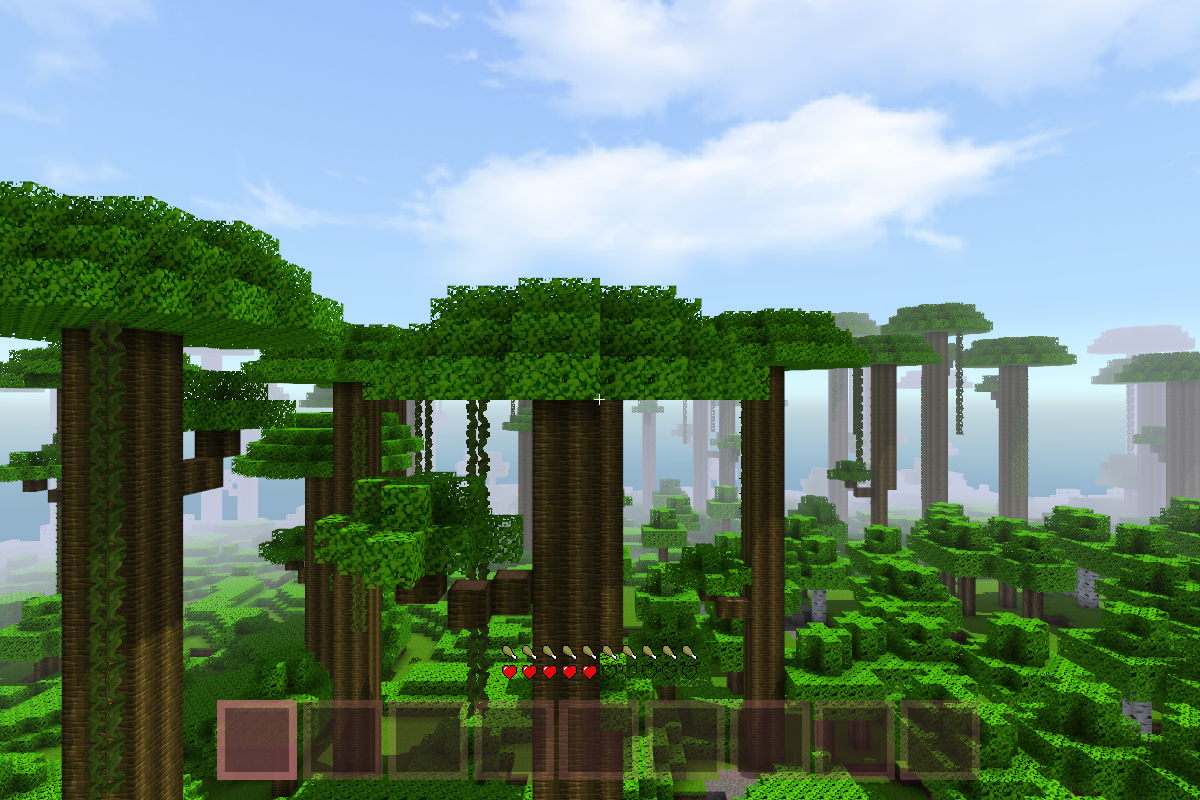
\includegraphics[width=.32\textwidth]{walk-2.png}
	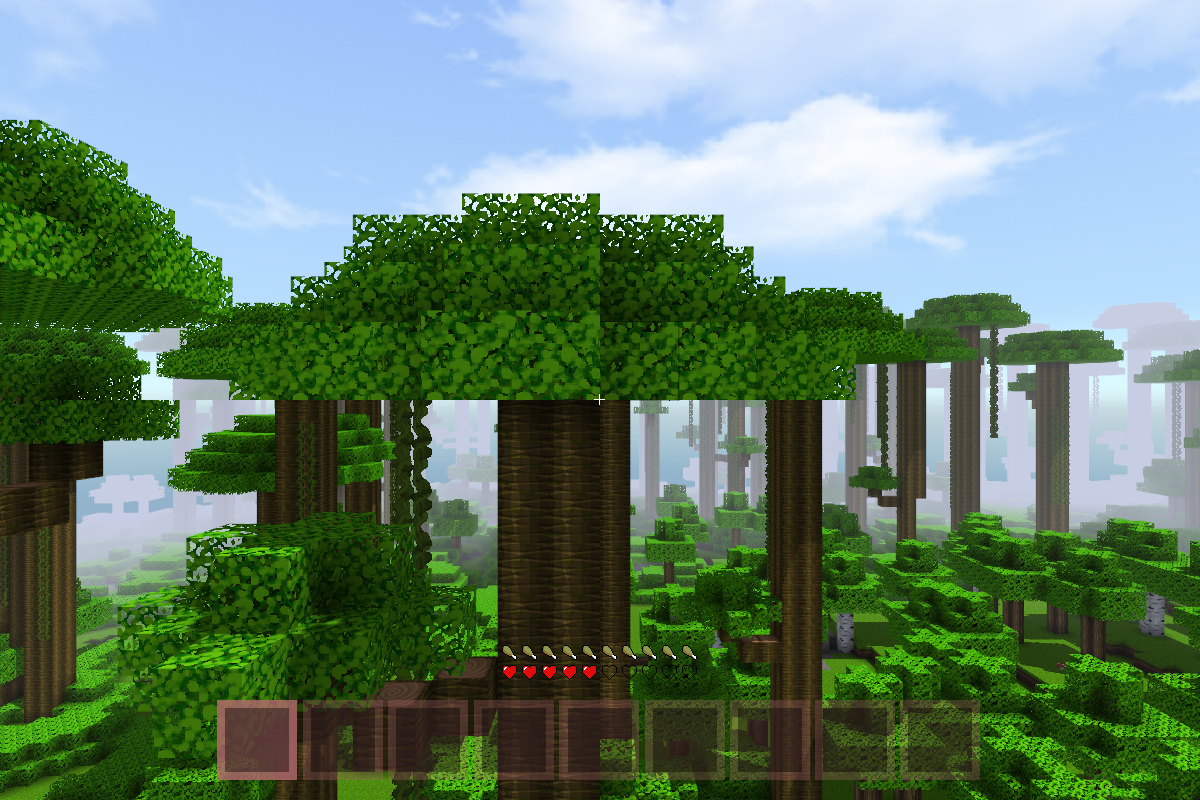
\includegraphics[width=.32\textwidth]{walk-3.png}
	\caption[Reihe von Screenshots, die die Fortbewegung in Szenario 5 zeigt.]{Reihe von Screenshots, die die Fortbewegung in Szenario 5 zeigt. Die Screenshots haben einen Zeitabstand von \SI{1000}{\milli\second}. Im Hintergrund sind die neu geladenen Chunks zu erkennen.}\label{fig:walk}
\end{figure}

Für die folgenden Messungen wird weiterhin der Seed 0 genutzt. Für dieses Szenario gibt es außerdem Messungen für die Seeds 3 und 10. Die Graphen dieser Messungen sind zusammen mit den Graphen der anderen Messungen gesammelt in Anhang~\vref{appendix:plots} zu sehen. Die Daten werden in Abschnitt~\ref{sec:zusammenfassung} mit den restlichen Daten zusammenfassend verglichen.

\paragraph{\ac{fps}}
Der Verlauf der Framerate in Szenario 5 wird von Abbildung~\ref{fig:seed-0-walk-fps} dargestellt. Wie in allen bisherigen Szenarien ist auch in Szenario Welt-Gehen Eine Verzögerung des Starts von SystemB im Vergleich zu SystemA zu erkennen.
\begin{figure}[!htbp]
	\fpsplot{seed-0-walk}
	\caption{Graph des Verlaufs der Framerate in Szenario 5: Welt-Gehen mit Seed 0.}\label{fig:seed-0-walk-fps}
\end{figure}
der Verlauf der Framerate ist in beiden Systemen deutlich unruhiger als in allen bisherigen Szenarien. SystemA erreicht im Durchschnitt \SI{128}{\fps}. In SystemB steigt die Bildwiederholrate um \SI{198}{\percent} auf durchschnittlich \SI{381}{\fps}. Während die Framerate in SystemA in etwa konstant bleibt, wenn man das unruhige Verhalten ausnimmt, steigt sie in System kontinuierlich langsam an. So wird zu Beginn eine Maximale Framerate von \SI{354}{\fps} gemessen. Diese steigt zum Schluss der Messung auf bis zu \SI{515}{\fps}. Der Grund dafür ist nicht bekannt. Es scheint allerdings nicht an der Beschaffenheit des Szenarios zu liegen, da dieses Verhalten in den Messungen mit den Seeds 3 und 10 (siehe Anhang~\vref{appendix:fpsplots}) nicht zu sehen ist.

\paragraph{\ac{cpu}}
Wie der Verlauf der Bildwiederholrate ist auch die Auslastung der \ac{cpu} deutlich unsteter als in den bisherigen Szenarien, in denen sie in der Hauptphase beinahe konstant ist. In Abbildung~\ref{fig:seed-0-walk-cpu} ist der Graph des Auslastungs-Verlaufs zu sehen.
\begin{figure}[!htbp]
	\cpuplot{seed-0-walk}
	\caption[Graph des Verlaufs der \glsentryshort{cpu}-Auslastung in Szenario 5: Welt-Gehen mit Seed 0.]{Graph des Verlaufs der \ac{cpu}-Auslastung in Szenario 5: Welt-Gehen mit Seed 0.}\label{fig:seed-0-walk-cpu}
\end{figure}
Im Gegensatz zu Szenario 4: Welt-Rotation, scheint die Messung in diesem Szenario in beiden Systemen zwar gleichzeitig zu sein. Dennoch ist der Trend der vorherigen Messungen einer längeren \ac{cpu}-Auslastung in der Anfangsphase auch hier nicht zu erkennen. Die Messungen mit anderen Seeds, die in Anhang~\vref{appendix:cpuplots} mit dargestellt sind, bestätigen dieses Ergebnis.

Zum ersten Mal steigt in diesem Szenario die Auslastung der \ac{cpu} auch während der Hauptphase In beiden Systemen immer wieder merklich an. SystemA hat eine durchschnittliche Auslastung von \SI{27}{\percent} und SystemB zeigt eine Durchschnittsauslastung von \SI{36}{\percent}. Dieser Anstieg ist auf die während der Hauptphase zu ladenden Chunks zurückzuführen. Hierfür werden in beiden Systemen alle Hardware-Threads genutzt, wie in den vorherigen Kapiteln beschrieben worden ist. Damit erhöht sich auch die Gesamtauslastung der \ac{cpu}. Dass in dem Graphen in der Hauptphase keine Auslastungsspitzen nahe \SI{100}{\percent} zu sehen sind, liegt vermutlich an einer zu geringen zeitlichen Auflösung der Messung.

\paragraph{\ac{gpu}}
Auch die \ac{gpu} erfährt in diesem Szenario eine variable Auslastung. Die Ausschläge sind, wie Abbildung~\ref{fig:seed-0-walk-gpu} zeigt, zwar nicht so groß wie in Szenario Welt-Rotation, dafür allerdings deutlich häufiger und nicht so regelmäßig.
\begin{figure}[!htbp]
	\gpuplot{seed-0-walk}
	\caption[Graph des Verlaufs der \glsentryshort{gpu}-Auslastung in Szenario 5: Welt-Gehen mit Seed 0.]{Graph des Verlaufs der \ac{gpu}-Auslastung in Szenario 5: Welt-Gehen mit Seed 0.}\label{fig:seed-0-walk-gpu}
\end{figure}
In SystemA lässt sich eine durchschnittliche Auslastung von \SI{34}{\percent} messen, SystemB zeigt \SI{42}{\percent} \ac{gpu}-Auslastung und damit eine Steigerung von \SI{24}{\percent}.

Auffällig ist, dass entgegen der Framerate die Auslastung der \ac{gpu} in SystemB während der Messung tendenziell sinkt. Dieses Verhalten lässt sich in den Messungen mit weiteren Seeds nicht reproduzieren (siehe Anhänge~\vref{appendix:fpsplots} und \vref{appendix:gpuplots}). Dort sind sowohl Framerate als auch \ac{gpu}-Auslastung, ausgenommen Schwankungen, gleichbleibend.

\paragraph{\ac{ram}}
Abschließend wird nun noch der in Abbildung~\ref{fig:seed-0-walk-mem} dargestellte Speicherverbrauch betrachtet. In beiden Systemen steigt der Tenured-Speicherverbrauch steigt an, während der Gesamtverbrauch über die gemessene Zeit in der Hauptphase konstant ist.
\begin{figure}[!htbp]
	\memplot[xticklabels={,,},xlabel={}]{seed-0-walk-single-mem.csv}
	\\\memplot{seed-0-walk-multi-mem.csv}
	\caption{Graph des Verlaufs der Speichernutzung in Szenario 5: Welt-Gehen mit Seed 0.}\label{fig:seed-0-walk-mem}
\end{figure} 
SystemA besitzt einen Speicherverbrauch von \SI{1215}{\mega\byte} und SystemB nutzt mit \SI{1881}{\mega\byte} durchschnittlich \SI{55}{\percent} mehr. Der kurzfristige Speicherverbrauch liegt bei \SI{114}{\mega\byte\per\second} in SystemA. Das ist das Maximum des Systems über alle Szenarien hinweg. In SystemB wird ein Speicherbedarf von \SI{248}{\mega\byte\per\second} für die Erzeugung kurzfristig genutzter Objekte gemessen. Damit ergibt sich in diesem Szenario ein Anstieg von \SI{118}{\percent}. 

Besonders interessant ist in diesem Szenario der Speicherverbrauch der langlebigen Objekte (Tenured). In allen anderen Szenarien ist diese Menge über den Großteil der Messung konstant.
In Szenario 5: Welt-Gehen steigt dieser zum ersten Mal während der Hauptphase stetig. In SystemA wird ein Anstieg von \SI{401}{\mega\byte} in Sekunde 25 zu \SI{705}{\mega\byte} in Sekunde 54 gemessen. In SystemB steigt die Nutzung von \SI{585}{\mega\byte} auf \SI{800}{\mega\byte}. Das ist ein dauerhafter Anstieg von \SI{10}{\mega\byte\per\second} in SystemA und ein Anstieg von \SI{7}{\mega\byte\per\second} in SystemB. Diese Tatsache liefert ein Indiz für die Existenz von Speicherlecks in der Blocklib. Um diesen Anschein zu bestätigen beziehungsweise zu entkräften, wäre es sinnvoll in der Zukunft auch längere Messungen durchzuführen. Eine mögliche Erklärung für den steten Anstieg wäre nämlich auch, dass in der Messung während der Hauptphase keine Garbage-Collection stattfindet und so nur scheinbar ein stetig steigender Speicherbedarf entsteht.



\pagebreak
\section{Fazit}
\pagebreak
\section{Ausblick}
\subsection{Etablierung einer Composition Root}
\begin{figure}
  \begin{center}
    \includesvg[]{Context-shortened.svg}
  \end{center}
  \caption{A}\label{fig:diagContext}
\end{figure}
\textcite[S.~76]{Seemann2012} definiert die \gls{compositionRoot} als (vorzugsweise) genau eine Position in einer Anwendung an der Module zusammengesetzt werden. Die korrekte Nutzung einer \gls{compositionRoot} impliziert die weite Verbreitung von \gls{dependencyInjection}, der Designarchitektur, in der Module ihre Abhängigkeiten nicht selbst erzeugen, sondern diese Aufgabe an aufrufende Module übertragen. Schlussendlich wird diese Aufgabe bis zur \gls{compositionRoot} weitergegeben, wo alle Abhängigkeiten aufgelöst werden. 


Das Design vieler Module in der Blocklib verfolgt häufig einen anderen Ansatz. Insbesondere Die abstrakte Klasse \class{Context} und die von ihr erbenden Klassen entsprechen eher einer Mischung aus \gls{servicelocator}~\cite[S.~301~ff.]{Nystrom2015} und \gls{singleton}~\cite[S.~103~ff.]{Nystrom2015}. Ein Klassendiagramm von \class{Context} ist in Abbildung~\vref{fig:diagContext} dargestellt. Die statische Methode \code{getInstance()} weist auf das \gls{singleton} Pattern hin. Die Klasse besitzt zwar keine Methode \code{resolve(...)}, wie es bei einem üblichen \gls{servicelocator} der Fall wäre, bietet aber stattdessen konkrete Methoden für die einzelnen Dienste, die es in der Blocklib gibt.

Sowohl das ursprüngliche \gls{singleton} Pattern von~\textcite[S.~127~ff.]{Gamma2016}, als auch das \gls{servicelocator} Pattern werden inzwischen teils kritisch betrachtet~\cite[S.~103~ff.]{Nystrom2015}\cite[S.~154~ff.]{Seemann2012}. Das liegt insbesondere daran, dass es beide Patterns ermöglichen, Module über die gesamte Code Basis hinweg zu koppeln, was es wiederum erschwert Auswirkungen von Änderungen im Code abzuschätzen. Des Weiteren erschwert besonders das \gls{singleton} Pattern von \class{Context} in der Blocklib das (Unit-) Testen. Nutzt eine Klasse \class{Context}, so ist es nahezu unmöglich, diese isoliert zu testen, da deren Methodenaufrufe sich durch den \class{Context} über die ganze Code Bases erstrecken können. Diese  Aufrufe können auch nicht durch \glspl{testdouble} (also spezielle Module, die das Verhalten von Komponenten vorspielen, damit die Originale beim Testen nicht benötigt werden) ersetzt werden, weil \class{Context} keine Möglichkeit bietet die bereitgestellten Dienste zu ersetzen. Außerdem kann im Test nicht festgestellt werden, welche Methoden überhaupt ersetzt werden müssten, da die Abhängigkeiten einer Klasse versteckt sind. Ruft eine Methode beispielsweise intern \code{Context.getInstance().getWorldInteraction()} auf, so ist das von außen nicht zu erkennen.

\subsubsection{Vorteile einer \glsentrytext{compositionRoot}}

Die Nutzung eines \gls{singleton} und \gls{servicelocator} ist zwar anfangs sehr angenehm, da jedes Modul nur einen Methodenaufruf entfernt ist, sie bringt aber auch die gleichen Probleme mit sich wie globale Variablen. Anders verhält es sich bei der Nutzung von \gls{dependencyInjection} über Konstruktoren und einer \gls{compositionRoot}. Im Folgenden sind kurz einige ihrer Vorteile erläutert.

\paragraph{Erkennung von Abhängigkeiten}Abhängigkeiten werden sichtbar, wenn die Klasse einen Konstruktor besitzt, der eine Instanz von \class{WorldInteraction} erwartet. Dann ist die Abhängigkeit offensichtlich. Es kann also einfach abgeschätzt werden, welche Änderungen Einfluss auf ein bestimmtes Modul haben. Zudem ist klar welche Bereiche beeinflusst werden können, wenn Methoden der Klasse aufgerufen werden, nämlich nur diejenigen zu denen sie auch eine Referenz besitzt.

\paragraph{Keine versehentlichen Abhängigkeiten} Außerdem wird die Gefahr verhindert aus Versehen, neue Abhängigkeiten aufzubauen, denn diese müssen explizit im Konstruktor angegeben werden. Bei einem \gls{servicelocator} reicht ein einfacher Methodenaufruf.

\paragraph{Das Testen wird vereinfacht} Es ist klar, dass die Klasse \class{WorldInteraction} genutzt wird, sie wird ja schließlich dem Konstruktor übergeben. Der Austausch von \class{WorldInteraction} durch ein Test Double ist trivial, da dieses einfach beim Aufruf des Konstruktors der Klasse übergeben werden kann. Dadurch lässt sich einfach eines der großen Probleme der Blocklib angehen -- eine fehlende automatisierte Testabdeckung. Aktuell muss bei den meisten Tests die gesamte Blocklib gestartet werden, sodass die Tests zu lange dauern, als dass man sie in häufigen Intervallen durchführen kann.

\textcite[S.~15~ff.]{Seemann2012} beschreibt noch einige weitere Vorteile der Nutzung von \gls{dependencyInjection}, darunter Erweiterbarkeit und die Möglichkeit leichter parallel Code zu entwickeln. Ein besonders wichtiger Punkt für die Blocklib ist zudem die verbesserte Wartbarkeit, da der Durchsatz an Entwicklerinnen und Entwicklern, die an der Blocklib arbeiten, sehr hoch ist.

\subsubsection{Mögliche Probleme bei der Umstellung}

Somit kann man davon ausgehen, dass die breite Etablierung der Nutzung von \gls{dependencyInjection} in Verbindung mit einer zentralen \gls{compositionRoot} erstrebenswert ist. Das Wort \enquote{breit} lässt allerdings bereits vermuten, dass diese Etablierung sehr viele Änderungen in der Blocklib hervorrufen wird. Im Folgenden wird nun beschrieben, welche potentiellen Probleme dabei in der Blocklib zu bewältigen sind.

\paragraph{Wo ist die \glsentrytext{compositionRoot}?}
Typischerweise soll die Komposition des Objektgraphen, also die Zusammensetzung der Module in der \gls{compositionRoot}, so nah wie möglich am Einstiegspunkt des Programms liegen~\cite[S.~232~ff.]{Martin17}\cite[S.~76~f.]{Seemann2012}. Das liegt daran, dass man dadurch die Entscheidung, wie die Komposition auszusehen hat und zugleich konkrete Abhängigkeiten, so lange wie möglich herauszögern kann. Man erreicht so also eine möglichst lose Kopplung der einzelnen Module des Programms.

Die Blocklib stellt nun einen besonderen Fall dar, da sie eigentlich nur eine Bibliothek darstellt. Der Programmeinstiegspunkt liegt also an einer anderen Stelle, nämlich in dem \class{BlockLibProgram}, das ausgeführt wird. Platziert man die \gls{compositionRoot} dort, besitzt jedes Programm völlige Freiheit, bei der Komposition der Blocklib. Allerdings ist dies dem Ziel abträglich, die Blocklib möglichst einfach nutzen zu können, zumal in den allermeisten Fällen die Komposition identisch sein wird. Einen Sonderfall stellt hier die Nutzung der Blocklib in der Multiplayer-Version dar, da hier tatsächlich beispielsweise für die Klassen \class{WorldInteraction} und \class{Context} spezielle Unterklassen vorhanden sind, die je nach Blocklib-Version verwendet werden. Alternativ kann man die Klasse \class{Game} als Einstiegspunkt betrachten, da hier bereit einige bibliotheksinterne Module komponiert werden und sie die Klasse ist, die in dem \class{BlockLibProgram} instanziiert wird. Sie stellt also den Einstiegspunkt für die Bibliothek dar. Wird die \gls{compositionRoot} allerdings hier platziert, verliert das \class{BlockLibProgram} allerdings die Möglichkeit der freien Konfiguration.

Wird die Blocklib in der Multiplayer-Version genutzt, entsteht ein weiteres Problem, da der gestartete Spring-Server keine Parameter übergeben bekommt. Es gibt nur einen Standardkonstruktor. Es muss also evaluiert werden, ob und wie Abhängigkeiten an den Server übergeben werden können. Ansonsten ist er von der \gls{compositionRoot} ausgeschlossen.

\paragraph{Aufwand der Umstellung ist nicht abzuschätzen}
Wie bereits erwähnt, wird die Etablierung einer \gls{compositionRoot} in der Blocklib sehr viele Änderungen hervorrufen, da beinahe jedes Modul über den \class{Context} verfügbar ist. Es lässt sich allerdings nicht abschätzen, wie hoch der Aufwand für eine Umstellung tatsächlich ist. Es gibt vielleicht Stellen, an denen das Design eines Moduls davon abhängt, dass es einen \class{Context} gibt, sodass das Modul komplett umstrukturiert werden muss. Andererseits kann es auch sein, dass die Umstellung nur die Erzeugung von geeigneten Konstruktoren erfordert und sehr simpel ist. Aufgrund der durch den \class{Context} versteckten Abhängigkeiten lässt sich das im Voraus nicht ermitteln, sondern wird sich erst bei der Durchführung zeigen.

\subsection{Dynamisches Rendern von Schrift}
\subsection{Thread Affinity}
\subsection{Jobsystem mit PriorityQueue}
\subsection{Konsolidieren des Jobsystems in der Simulation}
\subsection{Verstärktes Batching in der Simulation}
\printnoidxglossaries

\pagebreak
\printbibliography[title={Literaturverzeichnis},heading=bibintoc,notkeyword=online]

\pagebreak
\printbibliography[title={Quellenverzeichnis},heading=bibintoc,keyword=online] 


\appendix
\clearpage
\renewcommand{\sectionmark}[1]{\markboth{\Ifnumbered{section}{Anhang \thesection}{}}{#1}}
\pagenumbering{Roman}
\setcounter{page}{1}

\section*{Anhang}
\markright{Anhang}
\phantomsection
\addcontentsline{toc}{section}{Anhang}

Der beigelegte Datenträger enthält die folgenden Dateien.

\begin{itemize}
	\item PDF dieser Masterarbeit,
	\item Kompilierbare \LaTeX-Sourcen dieser Masterarbeit im Verzeichnis \code{latex} (Hinweis: Um die Arbeit vollständig neu kompilieren zu können, ist das Flag \code{--shell-escape} (manchmal auch write18) und die Software Inkscape\footnote{\url{https://inkscape.org/}} mit \code{PATH}-Eintrag nötig, da einige Grafiken externalisiert werden. Das Kompilieren der Arbeit dauert dann sehr lange. Die benötigten Grafiken sind im Ordner \code{latex-precompiled} bereits vorhanden. Dort ist das Flag nicht nötig),
	\item UML-Modelle als \code{.asta}-Dateien im Ordner \code{astah},
	\item den Source-Code im Verzeichnis \code{src}
	\item die Source-Code-Dokumentation im Ordner \code{doc},
	\item die bei den Messungen erstellten Rohdaten und verarbeitete Daten in den Ordnern\\ \code{latex(-precompiled)/performance/measurements},
	\item Skripte zur Verarbeitung der Daten in den Ordnern\\ \code{latex(-precompiled)/performance/measurements/python},
	\item Kopien von referenzierter Literatur und Quellen, die als PDF vorliegen im Ordner \code{recherche}.
\end{itemize}

\clearpage
\section{Klassendiagramme}
Dieser Abschnitt enthält einige Klassendiagramme, die detailliertere Informationen bereitstellen, als die in der Arbeit gezeigten.
\subsection{Executor im Concurrency Framework}\label{appendix:concFrameworkExecutor}
\includesvg[width=\textwidth]{ConcurrencyFrameworkExecutor.svg}

Wie in Abschnitt~\vref{sec:executor} beschrieben, erweitert das Interface \class{ExecutorService} das Interface \class{Executor} um eine Reihe von Methoden. Zum einen wird die Möglichkeit geboten den \code{submit(...)}-Methoden \class{Runnable}- oder auch \class{Callable}-Objekte zu übergeben, zum anderen bietet das Interface auch Methoden zur Verwaltung des Lebenszyklus des \class{ExecutorService}.

\clearpage
\subsection{\texttt{CompletionStage} im Concurrency Framework}\label{appendix:CompletionStage}
\includesvg[width=\textwidth]{CompletionStage.svg}

Klassendiagramm des Interface \class{CompletionStage}, auf das in Abschnitt~\vref{sec:CompletableFuture} verwiesen wird. Die definierten Methoden bieten verschiedene Möglichkeiten der Komposition.

\begin{tblr}{
	colspec={ll},
	row{1}={font=\bfseries}
	}
	Komposition & Methoden \\
	Verkettung & \code{thenApply(...)}, \code{thenAccept(...)}, \code{thenRun(...)}\\
	Zusammenführung & \code{thenCombine(...)}, \code{thenAcceptBoth(...)}, \code{runAfterBoth(...)} \\
	Auswahl & \code{applyToEither(...)}, \code{acceptEither(...)}, \code{runAfterEither(...)} \\
\end{tblr}

\clearpage
\subsection{\texttt{Context}}\label{appendix:context}
{
	\centering
	\includesvg[height=.7\textheight]{Context.svg}
	\par
}
Die Klasse \class{Context} besitzt, wie in Abschnitt~\vref{sec:EtablierungEinerKompositionroot} beschrieben, Methoden, um beinahe jedes System der Blocklib global für alle anderen Systeme verfügbar zu machen. 

Das ist zwar angenehm, da von überall aus leicht auf ein benötigtes System zugegriffen werden kann. Allerdings sind dadurch Abhängigkeiten zwischen Systemen schwieriger zu finden und Änderungen können unvorhergesehene Folgen haben, da beispielsweise irgendein anderes System die ursprüngliche Funktionalität genau so benötigt, wie sie davor war. 

\clearpage
\subsection{\texttt{BlocklibExecutorService}}\label{appendix:BlocklibExecutorService}
{
	\centering
	\includesvg[width=\textwidth]{ExecuterInterfaces.svg}
	\par
}
In Abschnitt~\vref{sec:designJobsystem} werden die hier dargestellten Interfaces besprochen. In dieser detaillierten Version des Klassendiagramms lässt sich nun erkennen, wie die jedes Interface die Schnittstelle, von der es abgeleitet ist, erweitert. Der \class{ScheduledExecutorService} Möglichkeiten des Scheduling hinzu und der neu definierte \class{BlocklibExecutorService} überschreibt zum einen den Rückgabewert der definierten Methoden und definiert zudem Kopien jeder Ausführungs-Methode mit dem zusätzlichen Parameter \code{priority} des Typs \class{TaskPriority}.

\clearpage
\section{Messungen}\label{appendix:plots}
\small
Dieser Abschnitt enthält die Graphen aller Messungen der Performanceanalyse (Kapitel~\ref{kap:performance}). Zur besseren Vergleichbarkeit sind diese nach der gemessenen Metrik gruppiert.
\vspace*{-.3em}\subsection{\glsentryshort{fps} Verläufe gesammelt}\label{appendix:fpsplots}
\pgfplotsset{
	height=1.4cm,
	every axis title/.append style={fill=white,at={(.0,1)},yshift=-.2cm,draw=black,anchor=south west,nodes={scale=.7}},
}
\settowidth\mytemp{1,}
\fpsplot[title={Szenario 1: Hexagon (0)},ytick={0,200,...,1200},height=2.8cm,ymax=1200,y label style={at={(ticklabel cs:.5,-\mytemp)}},xticklabels={,,},xlabel={}]{seed-0-hexagon}
\\[-.3em]\fpsplot[title={Szenario 2: Halb-Würfel (0)},xticklabels={,,},xlabel={}]{seed-0-cube}
\\[-.3em]\fpsplot[title={Szenario 3: Welt-Statisch (0)},xticklabels={,,},xlabel={}]{seed-0-static}
\\[-.3em]\fpsplot[title={Szenario 4: Welt-Rotation (0)},xticklabels={,,},xlabel={}]{seed-0-rotate}
\\[-.3em]\fpsplot[title={Szenario 5: Welt-Gehen (0)},xticklabels={,,},xlabel={}]{seed-0-walk}
\\[-.3em]\fpsplot[title={Szenario 5: Welt-Gehen (3)},xticklabels={,,},xlabel={}]{seed-3-walk}
\\[-.3em]\fpsplot[title={Szenario 5: Welt-Gehen (10)},]{seed-10-walk}\\[-.3em]
Dies ist die Darstellung aller Framerate-Verläufe. Das Szenario ist jeweils links oben am Graphen zu erkennen.

\clearpage
\subsection{\glsentryshort{cpu}-Auslastungs-Verläufe gesammelt}\label{appendix:cpuplots}
\pgfplotsset{
	height=1.9cm,
}

\cpuplot[title={Szenario 1: Hexagon (0)},xticklabels={,,},xlabel={}]{seed-0-hexagon}
\\[-.2em]\cpuplot[title={Szenario 2: Halb-Würfel (0)},xticklabels={,,},xlabel={}]{seed-0-cube}
\\[-.2em]\cpuplot[title={Szenario 3: Welt-Statisch (0)},xticklabels={,,},xlabel={}]{seed-0-static}
\\[-.2em]\cpuplot[title={Szenario 4: Welt-Rotation (0)},xticklabels={,,},xlabel={}]{seed-0-rotate}
\\[-.2em]\cpuplot[title={Szenario 5: Welt-Gehen (0)},xticklabels={,,},xlabel={}]{seed-0-walk}
\\[-.2em]\cpuplot[title={Szenario 5: Welt-Gehen (3)},xticklabels={,,},xlabel={}]{seed-3-walk}
\\[-.2em]\cpuplot[title={Szenario 5: Welt-Gehen (10)},]{seed-10-walk}\\[-.3em]
Dies ist die Darstellung aller \glsentryshort{cpu}-Auslastungs-Verläufe. Das Szenario ist jeweils links oben am Graphen zu erkennen.

\clearpage
\subsection{\glsentryshort{gpu}-Auslastungs-Verläufe gesammelt}\label{appendix:gpuplots}
\gpuplot[title={Szenario 1: Hexagon (0)},xticklabels={,,},xlabel={}]{seed-0-hexagon}
\\[-.2em]\gpuplot[title={Szenario 2: Halb-Würfel (0)},xticklabels={,,},xlabel={}]{seed-0-cube}
\\[-.2em]\gpuplot[title={Szenario 3: Welt-Statisch (0)},xticklabels={,,},xlabel={}]{seed-0-static}
\\[-.2em]\gpuplot[title={Szenario 4: Welt-Rotation (0)},xticklabels={,,},xlabel={}]{seed-0-rotate}
\\[-.2em]\gpuplot[title={Szenario 5: Welt-Gehen (0)},xticklabels={,,},xlabel={}]{seed-0-walk}
\\[-.2em]\gpuplot[title={Szenario 5: Welt-Gehen (3)},xticklabels={,,},xlabel={}]{seed-3-walk}
\\[-.2em]\gpuplot[title={Szenario 5: Welt-Gehen (10)},]{seed-10-walk}\\[-.3em]
Dies ist die Darstellung aller \glsentryshort{gpu}-Auslastungs-Verläufe. Das Szenario ist jeweils links oben am Graphen zu erkennen.

\clearpage
\subsection{\glsentryshort{ram}-Auslastungs-Verläufe gesammelt}\label{appendix:memplots}
  				\memplot[title={Szenario 1: Hexagon (0)},xticklabels={,,},xlabel={}]{seed-0-hexagon-single-mem.csv}
\\[-.2em]\memplot[xticklabels={,,},xlabel={}]{seed-0-hexagon-multi-mem.csv}
\\[-.1em]\memplot[title={Szenario 2: Halb-Würfel (0)},xticklabels={,,},xlabel={}]{seed-0-cube-single-mem.csv}
\\[-.2em]\memplot[xticklabels={,,},xlabel={}]{seed-0-cube-multi-mem.csv}
\\[-.1em]\memplot[title={Szenario 3: Welt-Statisch (0)},xticklabels={,,},xlabel={}]{seed-0-static-single-mem.csv}
\\[-.2em]\memplot[xticklabels={,,},xlabel={}]{seed-0-static-multi-mem.csv}
\\[-.1em]\memplot[title={Szenario 4: Welt-Rotation (0)},xticklabels={,,},xlabel={}]{seed-0-rotate-single-mem.csv}
\\[-.2em]\memplot[]{seed-0-rotate-multi-mem.csv}
\\[-.1em]\memplot[title={Szenario 5: Welt-Gehen (0)},xticklabels={,,},xlabel={}]{seed-0-walk-single-mem.csv}
\\[-.2em]\memplot[xticklabels={,,},xlabel={}]{seed-0-walk-multi-mem.csv}
\\[-.1em]\memplot[title={Szenario 5: Welt-Gehen (3)},xticklabels={,,},xlabel={}]{seed-3-walk-single-mem.csv}
\\[-.2em]\memplot[xticklabels={,,},xlabel={}]{seed-3-walk-multi-mem.csv}
\\[-.1em]\memplot[title={Szenario 5: Welt-Gehen (10)},xticklabels={,,},xlabel={}]{seed-10-walk-single-mem.csv}
\\[-.2em]\memplot[]{seed-10-walk-multi-mem.csv}\\[-.3em]
Dies ist die Darstellung aller \glsentryshort{ram}-Auslastungs-Verläufe. Das Szenario ist jeweils links oben am Graphen zu erkennen.
\end{document}